%%=====================================================================
%%  JFEC — Machine Learning special issue.  OFFICIAL OUP CLASS BUILD.
%%
%%  Content is identical to ../JFEC_A_Manuscript; only the class, the
%%  front matter and the preamble differ. Edit prose in sections/, which
%%  is shared in substance with that tree — keep the two in step.
%%
%%  LAYOUT. `modern, small` is the design the journal's own instructions
%%  recommend, and it is also one of the two the class leaves single
%%  column (cls:2519-2523) -- which the tables need, four of them
%%  carrying seven or eight columns of banded figures.
%%  `unnumsec` is NOT used: the body carries 65 \secref pointers and
%%  needs numbered heads.
%%=====================================================================
\documentclass[namedate,webpdf,modern,small]{oup-authoring-template}
%% The class sets \floatpagefraction=.94, which strands every figure behind the
%% [p] pipeline figure until the end of the document. Relax it so exhibits
%% appear where they are discussed (verified 2026-08-25: 42 -> 41 pages).
\renewcommand\floatpagefraction{.5}

%%=====================================================================
%%  preamble-oup.tex — the OUP port.
%%
%%  The class already provides: amsmath amssymb amsthm array caption
%%  graphicx hyperref multirow natbib rotating tikz xcolor url listings
%%  algorithm algpseudocode footmisc wrapfig tcolorbox subfloat.
%%  Do NOT reload any of them; several take options the class has set.
%%
%%  Dropped from the article-class preamble, because the class owns them:
%%    geometry fontenc inputenc lmodern microtype setspace  (page + fonts)
%%    natbib hyperref caption                               (refs + captions)
%%    the float-placement counters and \captionsetup        (class house style)
%%    the theorem environments                              (unused in the body)
%%  Kept from it: booktabs, threeparttable, mathtools, bm, float, and the
%%  whole macro block, which the sections depend on.
%%=====================================================================

% --- what the class does not supply ---------------------------------
\usepackage{booktabs}      % \cmidrule (16 uses) and \addlinespace (12); also
                           % supplies \bottomrule, which the class calls \botrule
\usepackage{threeparttable}% table notes under tables (30 uses)
\usepackage{mathtools}
\usepackage{bm}
\usepackage{float}
\usetikzlibrary{positioning,calc,fit,backgrounds,arrows.meta,shapes.geometric,decorations.pathreplacing,patterns}
\graphicspath{{figures/}}
\newcommand{\societylogo}{}  % the template defines this in its preamble

% --- cross-reference helpers (cleveref is not installed here) --------
\newcommand{\secref}[1]{Section~\ref{#1}}
\newcommand{\secsref}[2]{Sections~\ref{#1} and~\ref{#2}}
\newcommand{\tabref}[1]{Table~\ref{#1}}
\newcommand{\figref}[1]{Figure~\ref{#1}}
\newcommand{\eqnref}[1]{Equation~\eqref{#1}}
\newcommand{\appref}[1]{Appendix~\ref{#1}}
\newcommand{\panelref}[2]{Panel~#1 of \tabref{#2}}

% --- drafting helpers (delete before submission) ---------------------
\newcommand{\TODO}[1]{\textcolor{red}{[\textbf{TODO:} #1]}}
\newcommand{\PH}[1]{\textcolor{gray}{\ensuremath{\langle}\text{#1}\ensuremath{\rangle}}}
\newcommand{\PENDGROSS}{\TODO{pending gross-alignment verification}}
\newcommand{\PROVEN}{\textsc{[proven]}}
\newcommand{\SKETCH}{\textsc{[sketch]}}
\newcommand{\CONJ}{\textsc{[conjecture]}}

%%---------------------------------------------------------------------
%%  NOTATION — identical to the article-class build; the sections use it.
%%---------------------------------------------------------------------
\newcommand{\N}{N}
\newcommand{\Tw}{T}
\newcommand{\K}{K}
\newcommand{\Rmat}{\mathbf{R}}
\newcommand{\Cmat}{\mathbf{C}}
\newcommand{\Wmat}{\mathbf{W}}
\newcommand{\Dmat}{\mathbf{D}}
\newcommand{\Proj}{\mathbf{P}}
\newcommand{\Imat}{\mathbf{I}}
\newcommand{\rt}{\tilde{\mathbf{r}}}
\newcommand{\Zmat}{\mathbf{Z}}
\newcommand{\Lam}{\bm{\Lambda}}
\newcommand{\ones}[1]{\bm{1}_{#1}}
\newcommand{\Pgics}{\mathbf{P}_{\mathrm{GICS}}}
\newcommand{\SR}{\mathrm{SR}}
\newcommand{\Exp}{\mathbb{E}}
\newcommand{\Prob}{\mathbb{P}}
\newcommand{\Var}{\mathrm{Var}}
\newcommand{\Cov}{\mathrm{Cov}}
\newcommand{\real}{\mathbb{R}}
\newcommand{\tr}{\operatorname{tr}}
\newcommand{\rank}{\operatorname{rank}}
\DeclareMathOperator*{\argmin}{arg\,min}
\DeclareMathOperator*{\argmax}{arg\,max}
\newcommand{\Part}{\mathcal{P}}
\newcommand{\PartOne}{\Part_{\mathrm{one}}}
\newcommand{\PartRnd}{\Part_{\mathrm{rand}}}
\newcommand{\alphaFF}{\alpha_{\mathrm{FF5+MOM}}}
\newcommand{\ARI}{\mathrm{ARI}}
\newcommand{\nogroup}{\emph{no grouping}}
\newcommand{\randgroup}{\emph{random grouping}}


\begin{document}

\journaltitle{Journal of Financial Econometrics}
\DOI{DOI added during production}
\copyrightyear{2026}
\pubyear{2026}
\vol{00}
\issue{0}
\access{Advance Access Publication Date: Day Month Year}
\appnotes{Paper}
\firstpage{1}

\title[Quantifying the Contributions of Clustering in Statistical Arbitrage]{Quantifying the Contributions of Clustering in Statistical Arbitrage}

\author[1,$\ast$]{Lunji Zhu}
\author[2]{Yixuan He}
\author[1,3]{Mihai Cucuringu}

\address[1]{\orgdiv{Department of Mathematics}, \orgname{University of
California, Los Angeles}, \orgaddress{\state{California},
\country{United States}}}
\address[2]{\orgdiv{School of Mathematical and Natural Sciences}, \orgname{Arizona State University}, \orgaddress{\state{Arizona}, \country{United States}}}
\address[3]{\orgdiv{Department of Statistics and Oxford-Man Institute of Quantitative Finance}, \orgname{University of Oxford}, \orgaddress{\country{United Kingdom}}}

\corresp[$\ast$]{Corresponding author. \href{mailto:lunji@math.ucla.edu}{lunji@math.ucla.edu}.}

\received{Date}{0}{Year}
\revised{Date}{0}{Year}
\accepted{Date}{0}{Year}

\abstract{Clustering-based statistical arbitrage makes two decisions, the clustering and the trading model, usually evaluated together. We separate them by trading 12
clusterizers and two controls, no clustering and a random partition, on 27
years of large US equities, under a fixed cross-sectional rule and a neural trading head. Clustering adds alpha and cuts book
volatility by $28\%$ to $42\%$, while the trading head adds primarily alpha. The clusterizers disagree on the groups yet trade closely correlated books; their Sharpe-ratio differences arise mainly through volatility. Most of the 12 clusterizers retain alpha that factors and per-stock peer regressions together cannot explain.}
\keywords{statistical arbitrage, clustering, signed graphs, Sharpe ratio, factor models}

\keywords[JEL classification]{C58, G11, C38}

\maketitle

%!TEX root = ../main.tex
%%=====================================================================
%%  §1  INTRODUCTION          target 4-5 pp.
%%
%%  REWRITTEN 2026-08-21 on the v3 panel, to the JFEC house sequence
%%  (motivation -> literature -> gap/design -> contributions -> results
%%  -> roadmap). Two structural changes from the 2026-08-16 version:
%%   * the literature positioning is UNCOMMENTED and moved up. 9 of 9
%%     sampled JFEC introductions carry literature inside the intro.
%%   * contributions moved from 0.85 of the way in to 0.35, and turned
%%     from a nested enumerate into running ordinals. 0 of 9 sampled
%%     introductions use a list of any kind.
%%  NUMERALS: deliberately almost none. 5 of 9 sampled introductions
%%  report no numeric finding at all, and half of the figures the old
%%  version printed are either superseded on v3 or not yet independently
%%  recomputed. Every one of them now lives in the section or table this
%%  text points at. Do not reintroduce a numeral here without checking
%%  it against the exhibit that carries it.
%%  Voice: the author edits.
%%
%%  POSITIONING (unchanged, still binding):
%%   * brutti2026orthogonal ALREADY have a no-clustering control. Ours
%%     CORROBORATES; claim no priority. What their design cannot deliver
%%     is the moment decomposition (their P&L is normalized by its own
%%     standard deviation) and the partition-randomizing null (their
%%     placebo permutes within clusters, partition fixed).
%%   * guijarro2025deep report SR, mu and sigma per model. "We report
%%     volatility separately" is NOT a contribution.
%%
%%  FORBIDDEN HERE (each tested, each failed):
%%   - "every clustering earns the same alpha" (ANOVA rejects)
%%   - "the best method earns less alpha than no clustering"
%%   - any era rank-stability claim, in EITHER direction
%%   - any adjacent-pair ordering, any tradability claim
%%   - any point value for the head lift (bound only, +0.74 to +1.50)
%%   - any post-2009 alpha edge over K=1
%%   - "a clusterizer never sees a payoff" (false for four rules)
%%   - "forces/imposes group neutrality" (refuted, §4.3)
%%=====================================================================
\section{Introduction}
\label{sec:intro}

Machine learning methods are now used at most stages of trading
strategies \citep{kelly2023financial}, and clustering has become one of
the standard ways to form groups of comoving stocks for relative-value trading. First,
a clustering-based statistical arbitrage strategy partitions the stocks in the cross-section into several groups.
Then, a trading model builds trading portfolios on that partition, typically from returns hedged against the market. Previous studies in clustering-based trading usually evaluate the clustering algorithm and the trading model together and infer their effectiveness from the Sharpe ratio of the combined strategy \citep{Jinetal2023, LeeChang2026, brutti2026orthogonal}. However, the end-to-end performance does not identify which part makes what contribution. In this paper, we study what clustering contributes to statistical arbitrage. We call the clustering algorithm the clusterizer. First, we measure how much the clusterizer and the trading model contribute separately, and whether each contributes through the mean or through the volatilities of the payoffs. Second, we ask whether clusterizers based on different clustering rules recover different information. Third, we test whether traditional factor models, a reversal factor, or per-stock peer regressions, which regress each stock on the stocks most correlated with it, can provide the information that a clusterizer contributes.

The cluster structure of the stock market was studied long before cluster-based trading strategies were developed. The clusters can come from industry taxonomies, from the statistical structure of returns, and from a trading objective. Industry taxonomies fix the clusters in advance according to the economic characteristics of the companies
\citep{bhojraj2003whats}. The clusters can also be estimated from
returns, usually from the correlation matrix \citep{Mantegna1999}.
\citet{TOLA2008235} cluster the correlation matrix for portfolio construction.
\citet{Jinetal2023} apply the same idea to statistical arbitrage. Most recently, \citet{LeeChang2026} jointly fit
the partition and the model that trades based on it, via a transformer trained on a trading-based objective function.

A neighboring strand of literature asks how we can utilize the partitions for trading.
Early studies of relative-value trading include \citet{Gatevetal2006}, who documented the profitability of trading a single mean-reverting spread. Later, \citet{avellaneda2010statistical} replaced stock pairs with the factor-model residual, the part of a stock's return left after systematic factors are removed. It is worth noting that a cluster also provides another such factor, via the cluster mean. More recently, \citet{Jinetal2023}, \citet{LeeChang2026}, and
\citet{brutti2026orthogonal} each propose clusterizers of their own together with a strategy that gives trading portfolios based on their partitions. \citet{Jinetal2023} compare five spectral clusterizers, four of which are signed clusterizers that separate positive from negative correlations, under the same trading rule. In contrast, we separately analyze the contributions of clustering and of the trading rule within the whole trading pipeline.

To the best of our knowledge, no previous study compares clusterizers from different families under a common trading model, or separates what the partition contributes from what the model contributes. When the clusterizers and the trading rules are evaluated together, a higher Sharpe ratio may come from a better partition, from a better model, or from the way that the two match, so the end-to-end performance cannot help us examine the contribution of each component. Attribution also requires examining the mean and the volatility of the payoff separately. \citet{guijarro2025deep} examine both for factor-based statistical arbitrage. They report the Sharpe ratio, mean, and volatility of every model they fit and vary the factor construction under different signal models. However, they did not include clustering-based statistical arbitrage in their close examination.

We examine the clustering stage and the trading stage separately.
For the clustering stage, we compare 12 clusterizers from six families (geometric, hierarchical, eigenstructure-based, learned, trading-driven, and a sector taxonomy) against two controls.
The no-clustering control ($\K=1$) puts all stocks in a single group. The random-partition control is a uniform random partition with the same number of groups as the data-driven partitions. We call the partition of a clusterizer a real partition to contrast it with the random partition. Among the six families, we propose the trading-driven family and the learned family for the first time. In the trading-driven family, a clusterizer chooses its groups to optimize the Sharpe or Sortino ratio of the portfolio that a fixed trading rule builds on these groups. The learned family consists of \textsc{sssnet} \citep{he2022sssnet}, a signed-graph neural network that we bring to statistical arbitrage for the first time. We compare what the families' partitions contribute under a common downstream pipeline, without attempting to estimate the best attainable performance of each family of clusterizers.

For the trading stage, we trade every partition in a rule-based component and in a trained component. Each trading component builds a portfolio of long and short positions on a partition, and we call the daily return of this portfolio the payoff. The rule-based component uses a fixed cross-sectional rule adapted from \citet{Jinetal2023}. The trained component uses a neural trading head in the design of \citet{guijarro2025deep}, with the long convolution of \citet{fu2023simple} in place of their transformer. Because the fixed rule has no fitted parameter, the differences in performance among the rule-based portfolios come from the clustering stage alone. We then use the trained trading component to show how the conclusions change when a fitted model trades based on the partitions. We run both trading components on the same panel of daily returns for the 500 largest US equities over 27 years.

To attribute performance to the clustering stage and the trading stage, we compare the rule-based and trained components and use the two controls, replications under different random seeds, and a decomposition of the Sharpe gap. First, the two controls identify what the clustering stage contributes. The $\K=1$ control measures the cost of a missing partition. The random control measures the cost of wrong partitions. Second, the replications under different random seeds show whether different clusterizers can be distinguished in their partitions, positions, or payoffs. We compare partitions by the adjusted Rand index (\textsc{ari}), a measure of the agreement between two partitions corrected for chance. We judge gaps in the Sharpe-ratio ranking of the clusterizers against the dispersion of the design's own replications. In a head-seed rerun, the trading head is trained again from a different random initialization (a different head seed). In a partition draw, a stochastic clusterizer's daily partitions are generated again with a different random seed (a different partition seed). Third, the decomposition identifies whether a Sharpe gap arises through the mean payoff or through the payoff volatility. We split the gap
into the mean payoff part and the volatility part (\secref{sec:split}), because the same sample
estimates volatility more precisely than the mean (\secref{sec:resolution}).

We find that clustering lowers the volatility of the portfolio and raises its alpha, the intercept of a regression of the portfolio's payoff on the Fama--French five factors and momentum. First, demeaning market-hedged returns within the groups of a real partition removes the comovement that the stocks in each group share. With that comovement removed, the portfolio of a real partition is $39\%$ to $42\%$ less volatile than either control in the rule-based component and $33\%$ to $35\%$ less volatile in the trained component (\secsref{sec:hedge}{sec:mechanism}). Most of the Sharpe gap between a real partition and either control arises through this lower volatility (\secref{sec:split}). Second, demeaning within the groups of a real partition gives a more informative relative-value input than demeaning against the whole cross-section or within a random group. Consistent with this, we find that the two controls have the lowest alphas of the 14 rule-based portfolios (\secref{sec:hedge}).

With a fixed partition and at the same gross exposure, the trading head raises alpha in all 14 portfolios and raises volatility by proportionally less (\secref{sec:head}). Although the head widens the alpha advantage over both controls, especially over the random control, it narrows the volatility reduction. A wrong partition therefore has a larger disadvantage in the trained component than in the rule-based component, in the sense that the random control falls further behind the clusterizers in alpha.

In the trained component, the Sharpe-ratio ranking of the 12 clusterizers largely agrees with their ranking in the rule-based component. The ranking therefore reflects the quality of the partition as a trading input, whichever trading component trades it. However, some clusterizers in the middle of the ranking move by up to five places. The two controls also change order. In the rule-based component, the random control earns a higher Sharpe ratio than the $\K=1$ control. In the trained component, the two controls earn the same Sharpe ratio on average across head seeds (\secref{sec:head}).

We also find that the 12 clusterizers, which cluster stocks by qualitatively different principles, produce partitions that agree little by the \textsc{ari}. However, the portfolios built based on these partitions are highly correlated. The partitions are more alike in what demeaning within their groups removes than in how they group the stocks. For every clusterizer, demeaning within its groups removes much more comovement than the random control removes. By construction, the $\K=1$ control does not remove any comovement. Ten of the 12 clusterizers remove nearly the same share of the cross-sectional variance of market-hedged returns
(\secref{sec:mechanism}). The similarity between clusterizers also increases at each later stage of the pipeline, in the positions that the partitions induce and again in
the payoffs that those positions earn. In the payoffs, two different clusterizers differ
about as much as one clusterizer differs from its own head-seed rerun (\secref{sec:gradient}). Thus, the data clearly distinguish a real partition from the no-clustering and random controls, but provide much weaker separation among the clusterizers themselves. To the extent that the clusterizers' Sharpe ratios differ, they differ mainly through the volatility of the portfolios.

Most adjacent gaps in the Sharpe ranking are smaller than the variation of the gap itself across head-seed reruns (\secref{sec:field}). A stochastic clusterizer is unstable even across its own partition draws. Specifically, two partition draws of the same clusterizer disagree on group assignments nearly as much as two different clusterizers do. Moreover, the trading head enlarges the change in the Sharpe ratio that the redraw causes (\secref{sec:pseed}). Because the portfolios hold highly similar positions, re-selecting each year the clusterizer with the highest trailing Sharpe ratio does not outperform the equal-weight portfolio of all 12 clusterizers (\secref{sec:gradient}).

In contrast, changing the estimation window or the number of groups can change the Sharpe ratio by an amount of the same order as the gap between the best and the worst clusterizer. The estimation window is the trailing window of returns hedged against the market from which a clusterizer forms its groups. Between the best and the worst clusterizer, the gap in Sharpe ratio is $0.83$. We lengthen the estimation window from one month to one year. Over that range, the Sharpe ratio of unsigned spectral clustering rises by $0.88$, while that of average linkage is the same at both ends. We also reduce the number of groups from the $30$ used throughout to $10$. This change lowers the Sharpe ratio by up to $0.36$ (\secref{sec:window}).

Neither a factor model nor per-stock peer regressions make a partition redundant. \citet{guijarro2025deep} remark that latent factor estimation can, under appropriate assumptions, take the place of clustering. Taken as stated, the remark would make the clustering stage redundant, so we test it. We project the leading principal components, and separately the Fama--French factors, out of the day's cross-section of market-hedged returns. For each partition, we measure its variance share, the share of the cross-sectional variance of the day's market-hedged returns that demeaning within its groups removes. After either projection, every real partition loses at most $56\%$ of its variance share. No real partition falls to the variance share that a random partition would remove (\secref{sec:lens}).

We then test whether known return factors explain these alphas. We regress the payoff of every portfolio on the Fama--French five factors plus momentum and then add a short-term reversal factor and the five leading principal components of the market residuals. Every portfolio, including the two control portfolios, keeps a positive and significant alpha. The reversal factor explains at most $42\%$ of any portfolio's alpha, and it explains a larger share of alpha for the control portfolios than for the clusterizers' portfolios. To measure what a real partition adds, we also regress each clusterizer's portfolio and the random control's portfolio on the portfolio of the $\K=1$ control, which is the same pipeline run without clustering. Each clusterizer's portfolio keeps $41\%$ to $68\%$ of its alpha, whereas the random control's portfolio keeps $8\%$ to $9\%$ (\secref{sec:spanning}).

Because clustering-based trading is a special case of peer-based trading, in which every stock in a group shares the same peer set, we also compare it with per-stock peer regressions, in which each stock has its own peer set. In a per-stock peer regression, a stock's market-hedged return is regressed on those of the stocks most correlated with it, and the trading head trades the part that the regression does not explain. We build two such portfolios, which differ only in the number of days over which the regression is fitted. We call them the peer-regression portfolios. Peer regressions are a stronger substitute for a partition than the factors are.
In the cross-section, they absorb much of a partition's variance share, considerably more than the principal components or the Fama--French factors absorb. The peer regressions do not, however, fully absorb what the partitions earn. Against the peer-regression portfolios and the factors together, both controls lose their alpha. In contrast, most of the 12 clusterizers keep their alpha. Conversely, regressed on the equal-weight portfolio of all 12 clusterizers, both peer-regression portfolios keep their alpha (\secref{sec:peer}).

Finally, at a trading cost of five basis points per dollar traded, every daily-rebalanced portfolio, including the two control portfolios, has a negative net return (\secref{sec:costs}).

The rest of the article is organized as follows. In \secref{sec:lit}, we review the related literature. In \secref{sec:design}, we describe the panel, the 12 clusterizers, the two controls, and the rule-based and trained components. In \secref{sec:riskreturn}, we measure how clustering changes the volatility and the alpha of the portfolios and show how demeaning within groups lowers the volatility. We then split the Sharpe gap between the clusterizers and the controls into a mean part and a volatility part and measure what the trading head adds to the performance. In \secref{sec:invariance}, we compare the differences among the 12 clusterizers with the variation across head-seed reruns and partition draws. In \secref{sec:factor}, we test whether factor models or portfolios built on per-stock peer regressions explain the alphas of the clusterizers' portfolios. In that section, we also measure the effect of transaction costs. \secref{sec:conclusion} concludes. The appendix describes the construction of each clusterizer and the architecture and training schedule of the trading head. It also reports the additional results cited in the text.

%!TEX root = ../main.tex
%%=====================================================================
\section{Related Literature}\label{sec:lit}
%%=====================================================================
%%  HOUSE RULES FOR THIS SECTION (measured over four JFEC type-A
%%  literature sections; see _reference/LIT_PLAN.md).
%%   - NO \subsection, NO \paragraph labels. 0 of 4 corpus sections use
%%     any; structure is carried by ordinals in the prose, 4 of 4.
%%   - Every paragraph closes on a sentence about THIS article.
%%     11 of 20 corpus body paragraphs close first-person; 0 of 4
%%     sections close on a plain citation.
%%   - Gap claims are BOUNDED, never absolute ("comparisons are few",
%%     "first ... in the sense that"). A bare "none has done X" is a
%%     form the corpus never produces.
%%   - A hostile prior finding is reported straight and its diagnosis
%%     is HEDGED ("We reckon it is due to ..."), never disputed.
%%   - The nearest rival gets three clauses of credit BEFORE any
%%     difference is drawn, and the difference is a property of THEIR
%%     design, not an error.
%%   - The evaluation machinery is cited HERE, not only where used.
%%     That is the corpus norm and it is what keeps this section's
%%     citation load independent of the introduction's.
%%=====================================================================
This article combines two strands of previous work: methods for recovering peer-group structure from stock return time series, and modern statistical arbitrage strategies. In this section, we briefly review the literature in each strand, and highlight the gap that our work fills.

Industry taxonomies are the usual benchmark for a similarity-based
clustering, and the evaluation criterion is how much contemporaneous return
comovement the groups explain. Taxonomies such as the Standard Industrial Classification
(\textsc{sic}), the North American Industry Classification System
(\textsc{naics}), and the Global Industry Classification Standard
(\textsc{gics}) partition the cross-section
according to a classifying body's judgment about firms' primary lines
of business.
\citet{bhojraj2003whats} show that \textsc{gics} outperforms
\textsc{sic}, \textsc{naics}, and the 48-industry algorithm of \citet{FAMA1997153} on that
criterion; the other three perform similarly to one another, and the
\textsc{gics} advantage is sharpest among large firms.
\citet{chan2007industry} likewise find that within-industry comovement
is strongest among large caps, and that finer \textsc{gics} levels separate
comovement further. They also report that industry partitions are more homogeneous out of sample than groups obtained by statistical cluster analysis. Peers can also be
chosen firm by firm rather than read from a shared classification
\citep{bhojraj2002peer}, a construction we return to in \secref{sec:peer}.

The correlation matrix
of stock returns also contains information about market structure: the structure it encodes is hierarchical and tree-like
\citep{Mantegna1999, MantegnaStanley2000} and it behaves differently in
calm and in crash periods \citep{PhysRevE.68.056110}. That information can be extracted in several ways: by hierarchical linkage \citep{TOLA2008235}, by its spectrum \citep{macmahon2015community, rohe2011spectral}, and by
signed-graph methods that separate positive from negative correlation
\citep{cucuringu2019sponge, he2022sssnet, uddin2024network}. A partition is also a factor
model with grouped loadings \citep{ando2017clustering}, which is the form in which we later ask whether a factor model makes
%%  ⛔ SUBJECT MUST NOT BE GENERALIZED (CB, 2026-08-30). The sentence beginning\n%%  \"The linkage, spectral, and signed-graph methods all start...\" is true
%%  only of the linkage / spectral / signed-graph families. tab:methods row 1 has
%%  $k$-means on returns reading $\widetilde{\Rmat}$ DIRECTLY -- it forms no
%%  correlation matrix at all (same for the random control). Widening the subject to
%%  "the clusterizers" or "all methods" turns this into a false statement.
it redundant. A partition of the cross-section is used as a restriction in covariance estimation, where it is normally read from a taxonomy: \citet{alves2024forecasting} restrict the residual covariance of the S\&P~500 to ten \textsc{sic} sectors. The linkage, spectral, and signed-graph methods all start from the same correlation matrix; \secref{sec:invariance} and \secref{sec:factor} ask whether they recover different information from it, and whether what they recover survives a factor model or a per-stock peer regression. We study what a clusterizer contributes to
trading, holding the trading model fixed at each of two models in turn,
while 12 clusterizers and two controls read the same panel.

Machine learning has entered statistical arbitrage stage by stage. 
\citet{Gatevetal2006} formalize pairs trading as a
rules-based relative-value arbitrage and document its profitability
over decades of US data. The selection step has been automated by machine learning, from
return similarity \citep{SARMENTO2020113490} and from firm
characteristics \citep{HAN2023929}.
\citet{avellaneda2010statistical} replace the pair with a factor or ETF
decomposition and bet on an Ornstein--Uhlenbeck ``$s$-score'' built on
the residual. The trading model itself was then learned from data:
\citet{KRAUSS2017689} benchmark deep networks, gradient-boosted trees,
and random forests on lagged returns of the S\&P~500 cross-section,
\citet{FISCHER2018654} test long short-term memory networks on the same
data,
\citet{guijarro2025deep} learn the trading signal and its allocation
jointly on the residuals of a factor model, and \citet{epstein2025attention} learn the latent factors themselves
with an attention mechanism over firm characteristics. The models come from a wider machine learning program in asset pricing and financial econometrics
\citep{10.1093/rfs/hhaa009, kelly2019characteristics, zhang2024volatility, zhang2025graph}. Each applies machine learning to a different input of a trading
strategy: expected returns, factor loadings, volatility, and covariances. We take
one such model, a neural trading head trained on the Sharpe ratio of
its own book, and ask what it adds to a partition held fixed and
whether it erases the difference between a real partition and a random one.

The signal these strategies trade is a reversal, and the reversal literature has already found that demeaning within a group sharpens it. Short-term reversal itself dates to \citet{jegadeesh1990evidence} and \citet{lehmann1990fads}. \citet{da2014closer} find that sorting on returns within industries nearly doubles the return of the standard reversal strategy on large stocks, because industry momentum otherwise masks the reversal; \citet{hameed2015industries} document that intra-industry reversals are larger, more stable, and present among large liquid stocks, and decompose the unconditional reversal into intra- and inter-industry parts; and \citet{blitz2013residual} obtain a similar gain by reversing the residuals of a factor model. Our within-group demeaning is the same operation with the industry replaced by a statistical partition. These studies establish the value of conditioning reversal on economically or statistically related peers, but do not compare alternative grouping methods against both no-grouping and random-grouping controls; the two controls and the mean--volatility split of this paper supply that comparison. \secref{sec:spanning} then adds a market-wide reversal factor to the spanning regressions and finds that it absorbs more of the controls' alpha than of the clusterizers', far more at the rule-based component.

Clustering methods can also generate the partition-based residuals a statistical arbitrage strategy trades. \citet{Jinetal2023} first brought a signed spectral
method (\textsc{sponge}, \citealp{cucuringu2019sponge}) to statistical
arbitrage, on the correlation matrix of market residuals of US equities;
\citet{LeeChang2026} learn the clustering and the model that trades it
jointly, end to end, inside a transformer encoder on cryptocurrency
futures. \citet{brutti2026orthogonal} cluster return deviations with a noise-robust clusterizer, build
the partition to be orthogonal to the sector taxonomy, and show over
$2012$--$2024$ that the reversion payoff survives residualization against standard benchmarks; they also trade a no-clustering benchmark under the same rule. Comparisons across these studies are few, and those that exist either vary the clusterizer and the trading model together or, as in \citet{Jinetal2023}, compare variants within one family. We separate the two effects, ask whether clusterizers that disagree on the groups recover different information, and judge their ranking against the noise of the design's own replications. 
%!TEX root = ../main.tex
%%=====================================================================
%%  §4 "What the design can resolve" WAS FOLDED IN HERE on 2026-08-15
%%  and became §3.6. The old sections/04_resolution.tex is deleted.
%%  Reason on record: a standalone pre-results identification section is
%%  not a convention anything in _reference/VENUE/ supports, and at 3-4
%%  pages before any result it read as pre-emptive defence. The venue
%%  audit's complaint was body-vs-appendix, not a missing section.
%%  What did NOT come with it, and where it went:
%%    the pooled yardstick  -> §5 (sections/05_convergence.tex)
%%    the calibrated simulation -> §5.4, beside the era discussion
%%    the corr(SR,1/vol) refusal -> a footnote where volatility is
%%      first quantified
%%=====================================================================
%%=====================================================================
%%  §3  EVERYTHING FIXED BUT THE GROUPING      target 3-4 pp.
%%
%%  JOB. Make the reader believe that nothing varies except the object
%%  under study, and NAME THE OBJECT. This is the section the venue
%%  audit called structurally sound but foreign in voice: it currently
%%  reads as a data section. It should read as a design that isolates an
%%  estimand.
%%
%%  NAME THE ESTIMAND. A partition of the day's residual correlation
%%  matrix -- equivalently a restricted, one-hot loading matrix. Saying
%%  this once buys the whole paper its econometrics footing, and it is
%%  what makes §8's matched-rank comparison against principal components
%%  a non-nested comparison of two restricted factor structures rather
%%  than a horse race.
%%
%%  MUST CONTAIN:
%%   * panel: 6,941 OOS days, 1997-05-23 to 2024-12-30, top ~500 by cap
%%   * THE SPLIT-ADJUSTMENT CORRECTION. A credibility asset -- state it
%%     plainly in the body, do not bury it in a footnote. Facts, from
%%     NUMBERS.md N13.1:
%%       - the old panel built returns as pct_change() on prevAdjClose,
%%         which is off by the split factor on split days
%%       - most extreme recorded bad return: AIG on 2009-06-30 logged as
%%         +1644% against a true -12.78%
%%       - it was NOT noise. Reverse splits hit the names a mean-reversion
%%         book is LONG and forward splits hit the names it is SHORT, so
%%         BOTH SIGNS PAID THE BOOK. That sentence is the reason this
%%         belongs in the body: the error was biased in the strategy's
%%         favor, not symmetric around zero
%%       - corrected panel validated by asserting
%%         pct_change(fill_method=None) == returns.shift(1):
%%         max|diff| 1.776e-15 over 28,119,362 target cells
%%     ⚠ The effect on full-sample Sharpe -- "-0.069 to -0.144 SR across
%%       six naive streams", i.e. the old panel OVERSTATED Sharpes -- is
%%       only PARTIALLY VERIFIED. It is quoted from PROVENANCE.md; the
%%       underlying FINDINGS.md was never re-read and the six streams were
%%       never recomputed. ATTRIBUTE IT IN THE TEXT or drop the range and
%%       keep the AIG example, which is verified.
%%   * residualization: single-factor market model, 60-day rolling beta,
%%     computed ONCE, IDENTICAL across every configuration
%%     ⚠ the head residualizes for the SIGNAL but books RAW returns.
%%       Do not describe the strategy as "trading residuals"
%%   * the twelve methods by family, ONE sentence each -- the audit calls
%%     the long catalogue "a methods catalogue for a practitioner".
%%     Compress it; the detail goes to the appendix
%%   * THE TWO NULLS, and what each identifies:
%%       no clustering at all (K=1)    -> what clustering is worth
%%       random clustering (K=30)      -> what getting it wrong costs
%%     random falls BELOW no-clustering, which is why the two are not
%%     interchangeable. RECOMPUTED FROM DailyPnL 2026-08-15, both
%%     conventions, all 6,941 days:
%%       SR_mean   k1 1.4107 (n=3, sd 0.1198)   random 1.2662 (n=4, 0.1249)
%%       SR_avg    k1 1.5855                    random 1.4214
%%     ⚠ THE SIGN IS STABLE; THE SIGNIFICANCE IS NOT. At the seed level
%%       the gap (+0.1445) is smaller than either control's own seed s.d.
%%       and Welch gives t = 1.551, p = 0.187 -- NOT resolvable. On the
%%       seed-averaged daily series a circular block bootstrap (block 21,
%%       5,000 draws, seed 42) gives +0.1641, 95% CI [+0.0276, +0.3104],
%%       p = 0.016 -- resolvable. The two tests answer different
%%       questions (would a NEW SEED reverse it, versus do THESE two
%%       books differ over the sample). Report the ordering with its
%%       convention and its test; do NOT call it significant unqualified.
%%     ⚠ The conceptual point does not depend on the ordering at all:
%%       the two controls identify different things whichever is higher.
%%       Lead with that, and let the ordering be a measured detail.
%%   * the two trading layers: rule-based (no fitted parameter) and
%%     learned. Define "the book" and "gross exposure" -- foreign terms
%%     until defined
%%   * seeds: three per configuration, and why
%%   * validity: a run is invalid if ANY day has no long or no short.
%%     ⚠ "Four of eighty-five" is STALE -- the campaign has grown.
%%     Recomputed 2026-08-15 with ne_gate.discover() + gate_ok():
%%     151 runs discovered, FOUR fail, all on seed 7 (family_gics_seed7,
%%     family_random_seed7, kmeans_seed7, sssnet_seed7). The 151 includes
%%     the window and K sweeps, so SCOPE THE DENOMINATOR to the arm set
%%     the sentence is about rather than quoting a bare count.
%%   * ⚠ TWO STATISTICS ARE BOTH CALLED "SHARPE RATIO" here and differ
%%     by 0.14-0.27 -- RECOMPUTED 2026-08-15 across the common-window
%%     field, min +0.1418 (PCA loadings) max +0.2665 (SSSNET) mean
%%     +0.1791; NUMBERS.md N0.1 gives +0.1418..+0.2731 on SET19. The
%%     "0.15-0.17" that stood here and in the printed footnote was WRONG
%%     and understated the top end by 0.10. SR_avg > SR_mean always,
%%     because averaging seeds diversifies away head-training noise.
%%     Statistics: the mean of per-seed Sharpes (SR_mean) and the
%%     Sharpe of the seed-averaged payoff (SR_avg). Say which one every
%%     table uses. This is the single most reusable footgun in the paper
%%   * K is fixed NOMINALLY at 30 and not effectively: effective K runs
%%     8.68-28.89 over the seventeen nominal-K=30 arms
%%
%%  TABLE: the design table (rows = elements, columns = specification).
%%  Make "exactly one thing varies" visible.
%%
%%  ⛔ "Exactly one row varies" is FALSE as printed in the generated
%%     draft -- the correlation window is NOT common across the family
%%     (eleven arms at 60, five deliberate w21 twins, three at neither
%%     -- CORRECTED 2026-08-21 from label-cache evidence; the counts
%%     printed here were transposed). Say so
%%     here, and restrict every ranking exhibit to a common window.
%%=====================================================================
\section{Data and Experimental Design}
\label{sec:design}

In this section we hold every element of a statistical arbitrage
pipeline fixed except the clusterizer and the trading model, and we state what the resulting comparison estimates. A clustering-based statistical arbitrage strategy has two stages. A \emph{clusterizer} divides the cross-section of $\N_t$ stocks
into $\K$ groups: it maps the day's panel of residual returns to a
partition. A trading model then bets on relative value within each
group. We trade every partition under both a fixed cross-sectional rule and a
neural trading head. Throughout, \emph{clusterizer} denotes the algorithm, \emph{clustering} the operation it performs, and \emph{partition} the grouping it produces. The two-stage design---extract a
relative-value residual, then bet on it---follows the deep statistical
arbitrage line of \citet{guijarro2025deep} and
\citet{epstein2025attention}. Comparing partitions inside such a pipeline has precedents in \citet{Jinetal2023}, within the spectral family, and in \citet{brutti2026orthogonal}, whose no-clustering benchmark our rule-based results corroborate, though not its turnover (\secref{sec:costs}).

Write the day-$t$ partition $\Part_t$ as a membership matrix
%
\begin{equation}\label{eq:membership}
  \Zmat_t \in \{0,1\}^{\N_t \times \K},
  \qquad
  \Zmat_t \ones{\K} = \ones{\N_t},
\end{equation}
%
so that $[\Zmat_t]_{ik} = 1$ exactly when stock $i$ belongs to group $k$,
and the constraint records that every stock belongs to exactly one. The object we vary is $\Zmat_t$. It is formed from the panel of residual
returns and re-estimated every trading day. Equivalently, $\Zmat_t$ is a
factor loading matrix restricted to be one-hot: every stock loads on
exactly one group, with unit weight. An unrestricted
$\Lam_t \in \real^{\N_t \times \K}$ ($\K$ principal components,
say) lets every stock load on every component. Both are rank-$\K$
descriptions of the same cross-section, which makes them comparable.

Let $\pi_t(\Zmat)$ denote the payoff of the book the trading component produces from a partition $\Zmat$. We estimate the map
%
\begin{equation}\label{eq:estimand}
  \Zmat \;\longmapsto\; \bigl(\mu(\Zmat),\, \sigma(\Zmat)\bigr),
  \qquad
  \mu(\Zmat) = \Exp\bigl[\pi_t(\Zmat)\bigr],
  \qquad
  \sigma^2(\Zmat) = \Var\bigl[\pi_t(\Zmat)\bigr],
\end{equation}
%
and the organizing claim of this article is that clustering moves $\sigma$ more than it moves $\mu$. \figref{fig:pipeline}
draws the pipeline that produces $\pi_t$: every arm, one clusterizer or control traded at one component, shares
every stage except the partition. \secref{sec:factor} uses
the loading-matrix equivalence of \eqnref{eq:membership} directly,
comparing $\Zmat_t$ against principal components at matched rank~$\K$.

\begin{figure}[p]
\centering
\resizebox{\textwidth}{!}{% =====================================================================
%  Section 3, Figure 1 -- the design as a stratigraphic column.
%  Requires: tikz (arrows.meta, decorations.pathreplacing), graphicx,
%            amsmath, amssymb, xcolor, lmodern.
%  The four insets are resolved through \figinsetdir; leave it empty to
%  let \graphicspath{{figures/}} find them.
% =====================================================================
\providecommand{\figinsetdir}{figures/pipeline/}
\definecolor{figink}{HTML}{1A1A1A}
\definecolor{figrule}{HTML}{909090}
\definecolor{figgray}{HTML}{5C5C5C}
\definecolor{figvary}{HTML}{9A5410}
\definecolor{figvaryfill}{HTML}{FAF1E3}
\definecolor{figraw}{HTML}{1D5B8F}
\providecommand{\figts}{\fontsize{7.0bp}{8.1bp}\selectfont}% the 14-row arm table, whose row pitch is fixed
\providecommand{\figfs}{\fontsize{7.5bp}{8.6bp}\selectfont}% body text of the figure; \scriptsize (6.5bp) kept only in the estimand stratum, whose box is fixed
\begin{tikzpicture}[x=1pt,y=1pt,
    every node/.style={inner sep=0pt,outer sep=0pt},
    tx/.style={font=\figfs\linespread{0.96}\selectfont,align=left,
               anchor=north west,text=figink},
    gu/.style={font=\figfs\linespread{0.96}\selectfont,align=right,
               anchor=east,text=figink},
    gun/.style={font=\figfs\linespread{0.96}\selectfont,align=right,
               anchor=north east,text=figink},
    rb/.style={font=\figts,anchor=base west,text=figink},
    fb/.style={font=\figts\itshape,anchor=base east,text=figink},
    ic/.style={font=\figfs,align=right,anchor=north east,
               text=figgray},
    hair/.style={draw=figrule,line width=0.3pt},
    edge/.style={draw=figink,line width=0.45pt},
    tip/.style={-{Straight Barb[length=2.7pt,width=3.2pt]}}]
% ---------- horizontal geometry --------------------------------------
\def\GX{84}\def\MB{87}\def\SP{97}\def\CL{105}\def\CR{441}
\def\XL{90}\def\XR{447}\def\RW{435}
\def\IX{423}\def\IL{351}\def\IW{72}
\def\TR{326}
% ---------- stratum boundaries ---------------------------------------
\def\ya{0}\def\yb{-19}\def\yc{-39}\def\yd{-125}\def\ye{-265}
\def\yf{-335}\def\yg{-431}\def\yh{-463}\def\yi{-497}
% ---------- the one varied stratum, tinted ---------------------------
\fill[figvaryfill] (\XL,\yd) rectangle (\XR,\ye);
% ---------- stratum rules --------------------------------------------
\draw[draw=figink,line width=0.9pt] (\XL,\ya) -- (\XR,\ya);
\draw[hair] (\XL,\yb) -- (\XR,\yb);
\draw[hair] (\XL,\yc) -- (\XR,\yc);
\draw[draw=figvary,line width=0.8pt] (\XL,\yd) -- (\XR,\yd);
\draw[draw=figvary,line width=0.8pt] (\XL,\ye) -- (\XR,\ye);
\draw[hair] (\XL,\yf) -- (\XR,\yf);
\draw[hair] (\XL,\yg) -- (\XR,\yg);
\draw[hair] (\XL,\yh) -- (\XR,\yh);
\draw[draw=figink,line width=0.9pt] (\XL,\yi) -- (\XR,\yi);
% ---------- margin bar, thickened over the varied stratum ------------
\draw[draw=figrule,line width=0.5pt] (\MB,\ya) -- (\MB,\yi);
\draw[draw=figvary,line width=2.4pt] (\MB,\yd) -- (\MB,\ye);
% ---------- descent spine --------------------------------------------
\draw[edge] (\SP,-4) -- (\SP,-465);
\foreach \y in {-19,-38,-125,-265,-335,-431,-463}
  {\draw[edge,tip] (\SP,\y+5.5) -- (\SP,\y-2.5);}
\draw[edge,decorate,decoration={brace,amplitude=3.0pt,mirror}]
      (101,-337.5) -- (101,-428.5);
% ---------- the raw-return bypass ------------------------------------
\draw[draw=figraw,line width=0.9pt,dash pattern=on 2.7pt off 1.9pt,tip]
      (\RW,-3) -- (\RW,-437) -- (200,-437);
\node[font=\figfs,text=figraw,rotate=90,anchor=center] at (443,-232)
      {raw returns, untransformed};
% ---------- the inset column, lightly ruled off ----------------------
\draw[draw=figrule!50,line width=0.25pt] (341,\yc) -- (341,\yg);
% =====================================================================
%  gutter: how far the panel has been transformed
% =====================================================================
\node[gu]  at (\GX,-9.5)  {\textsc{panel} $r_{it}$};
\node[gun] at (\GX,-20.5) {\textsc{market}\\ \textsc{residual} $\tilde r_{it}$};
\node[gun] at (\GX,-41)   {\textsc{correlation} $\mathbf{C}$};
\node[gun] at (\GX,-128)  {\textsc{partition} $\mathbf{Z}_t$\\[1.0pt]
                           $K=30$, daily\\[3.0pt]
                           \textcolor{figvary}{\bfseries the only stage}\\
                           \textcolor{figvary}{\bfseries that varies}\\[1.0pt]
                           \textcolor{figvary}{$12+2=14$}\\
                           \textcolor{figvary}{configurations}};
\node[gun] at (\GX,-268)  {\textsc{group}\\ \textsc{demeaning} $s_{it}$};
\node[gun] at (\GX,-338)  {\textsc{the portfolio} $w_{it}$\\[1.0pt]
                           two trading models\\[1.0pt]
                           $\times\,2 = 28$ portfolios};
\node[gun] at (\GX,-434)  {\textsc{return} $\pi_t$};
\node[gun] at (\GX,-466)  {\textsc{moments} $\mu,\sigma$};
% =====================================================================
%  1. the panel
% =====================================================================
\node[tx] at (\CL,-1.5)
 {Daily US equities, top $500$ by market capitalization: raw returns $r_{it}$ on $N_t$ stocks.\\
  {\color{figgray}$6{,}913$ out-of-sample days, 8 July 1997--27 December 2024, shared by every configuration.}};
% =====================================================================
%  2. market residualization
% =====================================================================
\node[tx] at (\CL,-20.0)
 {$\tilde r_{it} = r_{it} - \hat\beta_{it}\,r_{mt}$,\quad
  $\hat\beta_{it}$ from the $60$ days $[t-59,t]$,\quad market $=$ SPY, a traded instrument.\\
  {\color{figgray}\itshape Computed before any partition exists: a common input, identical for every configuration.}};
% =====================================================================
%  3. the correlation object
% =====================================================================
\node[tx,text width=228pt] at (\CL,-44)
 {$\mathbf{C}$: the sample correlation of the market-residual
  panel $\widetilde{\mathbf{R}} = (\tilde r_{it})$, formed each trading day on the
  $60$-day estimation window.};
\node[tx,text width=228pt] at (\CL,-78)
 {{\color{figgray}\itshape Ten of the 14 configurations use $\mathbf{C}$ or a function of it. Of the other four, one uses $\widetilde{\mathbf{R}}$ directly and three use neither, although \textsc{gics} places the stocks outside its snapshot by correlation. Every configuration that uses $\mathbf{C}$ receives the same $\mathbf{C}$.}};
\node[anchor=north east] at (\IX,-42)
 {\includegraphics[width=\IW pt]{\figinsetdir corr_2014-07-07.pdf}};
\node[ic] at (\IX,-115.5) {$\mathbf{C}$ on 7 Jul 2014};
% =====================================================================
%  4. STAGE ONE -- the one object the article varies.
%     Rows are the fourteen arms; the second column is what each reads.
% =====================================================================
\node[tx,text=figgray,font=\figfs\itshape] at (164,-129) {clusterizer};
\node[tx,text=figgray,font=\figfs\itshape] at (262,-129) {input};
\draw[draw=figvary!60,line width=0.4pt] (\CL,-139) -- (\TR,-139);
\draw[draw=figvary!45,line width=0.3pt]  (254,-140) -- (254,-262);
\foreach \y in {-150.1,-167.3,-193.1,-201.7,-236.1}
  {\draw[draw=figvary!35,line width=0.25pt] (\CL,\y) -- (\TR,\y);}
\draw[draw=figvary!55,line width=0.3pt,dash pattern=on 1.3pt off 1.4pt]
      (\CL,-244.7) -- (\TR,-244.7);
\node[fb] at (156,-147.8) {Geometric};
\node[fb] at (156,-160.7) {Hierarchical};
\node[fb] at (156,-182.2) {Eigenstructure};
\node[fb] at (156,-199.4) {Learned};
\node[fb] at (156,-220.9) {Trading-driven};
\node[fb] at (156,-242.4) {Taxonomy};
\node[fb,text=figvary] at (156,-255.3) {Controls};
\foreach \y/\r/\d in {%
  -147.8/{$k$-means on residuals}/{$\widetilde{\mathbf{R}}$},
  -156.4/{average linkage}/{$\mathbf{C}$},
  -165.0/{complete linkage}/{$\mathbf{C}$},
  -173.6/{spectral (unsigned)}/{$|\mathbf{C}|$},
  -182.2/{PCA loadings}/{eig $\mathbf{C}$},
  -190.8/{\textsc{sponge}$_{\mathrm{sym}}$}/{$\mathbf{C}^{+},\mathbf{C}^{-}$},
  -199.4/{\textsc{sssnet}}/{signed $\mathbf{C}$},
  -208.0/{Sharpe}/{$\mathbf{C}$ and $\widetilde{\mathbf{R}}$},
  -216.6/{Sortino}/{$\mathbf{C}$ and $\widetilde{\mathbf{R}}$},
  -225.2/{Sharpe (EWMA)}/{$\mathbf{C}$ and $\widetilde{\mathbf{R}}$},
  -233.8/{Sharpe (graph)}/{$\mathbf{C}$ and $\widetilde{\mathbf{R}}$},
  -242.4/{\textsc{gics}}/{nothing, where covered},
  -251.0/{$K=1$ (no clustering)}/{nothing},
  -259.6/{random partition}/{nothing}}
  {\node[rb] at (164,\y) {\r};
   \node[rb] at (262,\y) {\d};}
\fill[white] (\IL,-131.4) rectangle (\IX,-247.6);
\node[anchor=north east] at (\IX,-131.9)
 {\includegraphics[width=\IW pt]{\figinsetdir zmat.pdf}};
\node[ic] at (\IX,-248.6) {$\mathbf{Z}_t$, the same day};
% =====================================================================
%  5. peer demeaning -- the second residualization
% =====================================================================
\node[tx] at (\CL,-268)
 {$s_{it} = \tilde r_{it} - |C_{k(i)}|^{-1}\sum\nolimits_{j \in C_{k(i)}} \tilde r_{jt}$};
\node[tx,text width=228pt] at (\CL,-285)
 {{\color{figgray}\itshape The market is removed above. The mean of the stock's group is removed here.
   In a group of size one, $s_{it}$ is zero, so the portfolio does not trade that stock on that day.}};
\node[anchor=north east] at (\IX,-267.6)
 {\includegraphics[width=\IW pt]{\figinsetdir demean.pdf}};
\node[ic] at (\IX,-322.8) {group means, 7 Jul 2014};
% =====================================================================
%  6. STAGE TWO -- pinned, run in two variants
% =====================================================================
\node[tx,text width=228pt] at (\CL,-338)
 {\textbf{(a) Fixed trading rule.} Five-day sum of $s_{it}$, sign flipped: long what has underperformed its group, short what has outperformed it, equal weight each side. Gross $1$, net $0$: dollar neutral by construction, with no fitted parameter.};
\draw[draw=figrule,line width=0.25pt,dash pattern=on 1.2pt off 1.4pt]
      (\CL,-378) -- (333,-378);
\node[tx,text width=228pt] at (\CL,-380)
 {\textbf{(b) Neural trading head.} Thirty-day path of running sums of $s_{it}$, one channel
  per stock; parallel kernel widths $2,4,8$ into a long-convolution head, no attention.
  $\sum\nolimits_i |w_{it}| = 1$ fixes gross and leaves net free, so the portfolio is not dollar neutral. Refitted
  walk-forward every $125$ days; five head seeds.};
\node[anchor=north east] at (\IX,-347.4)
 {\includegraphics[width=\IW pt]{\figinsetdir signal.pdf}};
\node[ic] at (\IX,-409.1) {$s_{it}$ paths, 7 Jul 2014};
% =====================================================================
%  7. the payoff -- settled in raw returns
% =====================================================================
\node[tx] at (\CL,-433)
 {$\pi_t = \sum\nolimits_i w_{it}\, r_{i,t+1}$};
\node[tx] at (\CL,-449)
 {{\color{figgray}\itshape Market residuals build the partition and the signal. The portfolio earns raw returns.}};
% =====================================================================
%  8. the estimand -- the pair, measured separately
% =====================================================================
\node[tx,font=\scriptsize\linespread{0.96}\selectfont] at (\CL,-465)
 {The estimand is the map $\mathbf{Z}\mapsto\bigl(\mu(\mathbf{Z}),\sigma(\mathbf{Z})\bigr)$.
  We report its two parts separately.};
\draw[draw=figink,line width=0.45pt] (\CL,-479) rectangle (\CR,-493);
\draw[draw=figink,line width=0.45pt] (273,-479) -- (273,-493);
\node[font=\scriptsize\selectfont,anchor=west,text=figink] at (112,-486)
 {$\mu(\mathbf{Z}) = \mathbb{E}\bigl[\pi_t(\mathbf{Z})\bigr]$:
  {\itshape\color{figgray}the mean return}};
\node[font=\scriptsize\selectfont,anchor=west,text=figink] at (280,-486)
 {$\sigma(\mathbf{Z}) = \operatorname{sd}\bigl[\pi_t(\mathbf{Z})\bigr]$:
  {\itshape\color{figgray}its volatility}};
\end{tikzpicture}
}
\caption{The strategy pipeline. This figure shows the stages of the pipeline as horizontal bands, one per stage. The arms differ only in the partition band, whose second column lists the input each clusterizer uses; every other band is common to all arms. Raw returns bypass the residual construction and re-enter at the payoff. The four insets are computed from the panel and from the $k$-means partition the runs used ($\K=30$, re-estimated daily) for 7~July 2014, a day with $\N_t = 500$ names, all 30 groups occupied, the largest holding $78$ names and six holding one, which carry no position. $\Cmat$ is ordered by that day's groups; $\Zmat_t$ is the membership matrix with columns sorted by group size. The paths are 26 of the $478$ eligible names, 30 days of cumulative peer-demeaned residual return in percent, with the five days the rule-based component reads shaded.}
\label{fig:pipeline}
\end{figure}

\subsection{The Panel}
\label{sec:panel}

We build the panel from daily CRSP data obtained through WRDS, covering
1990 to 2024. The traded universe is the 500 names
with the largest market capitalization as of the \emph{previous} close,
reselected daily. This restriction keeps the comparison in a large, liquid-equity universe while allowing membership to evolve using only information available at the previous close. The names must be common stock with a full residual history over the estimation window.\footnote{CRSP share codes $10$, $11$, and $12$.} The return is CRSP's close-to-close return adjusted for splits and dividends. Every result in this article is computed on the $6{,}913$ out-of-sample trading days that all 14 arms (the 12 clusterizers and the two controls) share at both trading components, 8 July 1997 to 27 December 2024. The neural trading head is pre-trained on the first $1{,}000$ days on which a book can be
formed, and the walk-forward loop begins on the day after the last of them. The panel's date labels run one trading day ahead of the Fama--French calendar; the offset is corrected before any regression on the factor file, and no statistic computed within the panel depends on it (\appref{app:calendar}). 

%%  ⚠ DECISION PENDING (2026-08-15). The split-adjustment material was
%%  drafted in the body and MOVED to Appendix A.1 at the author's
%%  instruction, leaving the pointer sentence above. A \TODO in
%%  A_supplementary.tex asks the coauthors to settle body vs footnote vs
%%  appendix. If it comes back to the body, the full text is in the
%%  appendix file and can be moved back intact.

\subsection{Residualization}
\label{sec:resid}

To remove the market factor, we residualize every stock's return
against the S\&P~500 exchange-traded fund (SPY) using a single-factor
market model. 
Writing $r_{it}$ for the raw return on stock $i$ and $r_{mt}$ for the
market return,
%
\begin{equation}\label{eq:residual}
  \tilde r_{it} \;=\; r_{it} - \hat\beta_{it}\, r_{mt},
  \qquad
  \hat\beta_{it}
  \;=\;
  \frac{\widehat{\Cov}_{[t-59,\,t]}\bigl(r_i,\, r_m\bigr)}
       {\widehat{\Var}_{[t-59,\,t]}\bigl(r_m\bigr)},
\end{equation}
%
the estimation window running over the 60 trading days ending at $t$
inclusive; the window length follows \citet{avellaneda2010statistical}. The ratio in \eqnref{eq:residual} is the least-squares slope from a regression of $r_i$ on $r_m$ with an intercept; the intercept is not subtracted, so $\tilde r_{it}$ is a market-hedged return, which we call a ``residual'' for brevity, rather than the regression residual itself. The position formed at the close of day $t$ earns $r_{i,t+1}$, which lies outside every estimation window, so no position uses information about the return it earns; the convention is shared by all 14 arms.\footnote{Ending the window at $t-1$ instead, with every partition held fixed and the trained component not rerun, moves each rule-based book's Sharpe ratio by less than $0.04$, well inside the dispersion of \secref{sec:field}. The volatility reduction from clustering is unchanged to the first decimal and the alpha advantage over either control is marginally larger, so the convention retained here is conservative.}

\eqnref{eq:residual} involves no $\Zmat_t$ and is computed
once. The residual panel $\widetilde{\Rmat} = (\tilde r_{it})$ is therefore a common input: every
clusterizer is the map $\widetilde{\Rmat} \mapsto \Zmat_t$
evaluated at the same argument. The residuals drive the clustering and the trading signal, but the book
is settled in raw returns: $\pi_t$ in \eqnref{eq:estimand} accumulates
$r_{it}$, not $\tilde r_{it}$.


\subsection{The Clusterizers}
\label{sec:methods}

We compare the 12 clusterizers, using a common 60-day estimation window wherever the partition is estimated from returns or correlations.
\tabref{tab:methods} lists them by
family, with what each clusterizer reads and how each is
constructed.\footnote{The list omits density-based clustering (DBSCAN, OPTICS), standard in
pairs selection since \citet{SARMENTO2020113490}, because it returns a variable number of clusters and discards unclustered names, which a design matching $\K$ across arms cannot accommodate; \appref{app:singleton} finds the cost of discarding names inside the noise of a single refit. Modularity-based community detection also chooses its own $\K$, and single-linkage clustering is omitted for chaining.} Each clusterizer receives the same
$\widetilde{\Rmat}$, targets the same $\K$, and passes its $\Zmat_t$ to the same trading stage. $\K$ is $30$ throughout, the fixed-$\K$ benchmark of \citet{Jinetal2023}; \appref{app:ksweep} sweeps it. We do not tune any clusterizer's settings to its trading results. Each runs at one pre-specified setting,
because the question is how much a downstream Sharpe ratio can tell apart different partitions, not which setting of any one method is
best. \appref{app:rules} gives each clusterizer's construction, and
\appref{app:sizes} the partitions it produces.

\begin{table}[htbp]
\centering
\caption{The 12 clusterizers}
\label{tab:methods}
\begin{threeparttable}
\footnotesize
\setlength{\tabcolsep}{3pt}
\renewcommand{\arraystretch}{0.96}
\begin{tabular}{@{}l>{\raggedright\arraybackslash}p{2.6cm}c>{\raggedright\arraybackslash}p{4.65cm}@{}}
\toprule
Clusterizer & Reads & Window (days) & Construction \\
\midrule
\multicolumn{4}{@{}l}{\emph{Geometric}}\\
$k$-means on returns & $\widetilde{\Rmat}$ directly & $60$
  & $k$-means on the residual return vectors in Euclidean space;
    forms no correlation matrix \\
\addlinespace
\multicolumn{4}{@{}l}{\emph{Hierarchical} \citep{Mantegna1999, TOLA2008235}}\\
Average linkage & $\Cmat$ & $60$
  & agglomerative clustering on $\Dmat = 1 - \Cmat$ \\
Complete linkage & $\Cmat$ & $60$
  & the same, complete rather than average linkage \\
\addlinespace
\multicolumn{4}{@{}l}{\emph{Eigenstructure} \citep{macmahon2015community, cucuringu2019sponge}}\\
Spectral (unsigned) & eigenvectors of $|\Cmat|$ & $60$
  & spectral clustering on the unsigned correlation \\
PCA loadings & eigenvectors of $\Cmat$ & $60$
  & $k$-means on the 10 leading eigenvector coordinates \\
\textsc{sponge} & a signed-Laplacian pencil & $60$\tnote{a}
  & the symmetric variant \textsc{sponge}$_{\text{sym}}$, on the positive
    and negative parts of $\Cmat$; unlike the row above it uses the
    sign\tnote{b} \\
\addlinespace
\multicolumn{4}{@{}l}{\emph{Learned} \citep{he2022sssnet}}\\
\textsc{sssnet} & $\Cmat$, as a signed graph & $60$
  & a signed-graph network trained on a clustering objective,
    warm-started from \textsc{sponge}\tnote{c} \\
\addlinespace
\multicolumn{4}{@{}l}{\emph{Trading-driven}}\\
Sharpe & $\Cmat$ and the payoff & $60$
  & a soft assignment optimized against the realized Sharpe ratio of
    the book it produces, hardened by $\arg\max$ \\
Sortino & $\Cmat$ and the payoff & $60$
  & the same, downside deviation replacing the standard deviation \\
Sharpe (EW) & $\Cmat$ and the payoff & $60$
  & the same objective exponentially weighted, decay $0.99$\tnote{d} \\
Sharpe (graph) & $\Cmat$ and the payoff & $60$
  & the assignment comes from a signed-graph network, and the objective
    matches the trading signal's 30-day horizon \\
\addlinespace
\multicolumn{4}{@{}l}{\emph{Taxonomy} \citep{bhojraj2003whats}}\\
\textsc{gics} & nothing, on the names it
  covers & --- & a static sector classification; names outside the table are
    placed by correlation\tnote{e} \\
\addlinespace
\midrule
\multicolumn{4}{@{}l}{\emph{Controls}}\\
No clustering ($\K=1$) & nothing & ---
  & one all-market group, so the trading rule demeans against the whole
    cross-section \\
Random partition & nothing & ---
  & a uniform random partition redrawn each day, matched to the real partitions in $\K$ \\
\bottomrule
\end{tabular}
\begin{tablenotes}[flushleft]\footnotesize
\item \emph{Notes.} This table lists the 12 clusterizers, the object each reads, its estimation window, and its construction. Every clusterizer receives the same $\widetilde{\Rmat}$ and targets the
same $\K$. Identifiers used in the runs are given in \appref{app:names}.
\item[a] Every clusterizer that forms a correlation matrix reads the same
60 trading days. \textsc{sponge} is estimated at 21 days in its
original implementation; the arm carried here is its 60-day variant, so that a comparison across clusterizers is not a comparison of windows.
The substitution does not disadvantage \textsc{sponge}
(\appref{app:names}). The three arms
marked --- form no correlation matrix at all.
\item[b] Groups of fewer than two members are handled differently:
\textsc{sponge}, Sharpe, and Sortino reassign such a member to its most
correlated group, while the other nine clusterizers leave it and the trading
stage drops it. For the three that reassign this is immaterial; under $k$-means on returns, the one clusterizer with a material singleton rate, the deletion changes the traded book, and \appref{app:singleton} measures its cost.
\item[c] Run once to produce a fixed set of daily partitions used by all five seeds, like the other stochastic clusterizers (\appref{app:sssnet}).
%% v3-VERIFIED 2026-08-20 (coverage 54-73%, fill ~35%, exactly 10 groups):
%% measured from partitions_v3/labelcache_gics vs labelcache_kmeans_ret over the
%% 6,944 OOS days. Do NOT restore the old-panel 48-68 / 40 / 10.9 in the number pass.
\item[d] Sharpe (EW) differs from Sharpe in more than the weighting, so the
clean contrast is Sharpe against Sortino.
\item[e] The table is a single snapshot covering roughly $54\%$ to $73\%$ of the
universe by era, so it carries survivorship and coverage bias by construction.
The names it does not cover, about $35\%$ of the book on a given
day, are assigned to the group they correlate with most strongly, so the arm that is
actually traded is a taxonomy--correlation hybrid; the \emph{Reads} column records the taxonomy alone. 
\end{tablenotes}
\end{threeparttable}
\end{table}

Three features of the list matter later. First, the families differ in the information they use as well as in the algorithm, and the window experiment of \secref{sec:window} finds sensitivity to the length of the estimation window concentrated in the clusterizers that read individual eigenvectors of the correlation matrix. Second, the four trading-driven clusterizers optimize the
partition against the Sharpe or Sortino ratio itself rather than against any other measure of
cluster quality. Whether using the payoff helps is then an empirical question, and with our design it does not: one of the four finishes near the top of the ranking and three in the lower half (\secref{sec:field}). Third, we include \textsc{gics} to give the
comparison a non-statistical reference point, and carry its coverage
caveat (\tabref{tab:methods}, note e) wherever it appears.


\subsection{The Two Trading Components}
\label{sec:components}

We trade every partition twice: once by a fixed cross-sectional rule
with no fitted parameter, and once by a neural trading head fitted on a Sharpe ratio loss. Both components begin by demeaning within the same partition: on each day we
subtract from every stock's residual the average residual of its own
group,
%
\begin{equation}\label{eq:relsig}
  s_{it} \;=\; \tilde r_{it} \;-\; \frac{1}{|C_{k(i)}|}
               \sum_{j \in C_{k(i)}} \tilde r_{jt},
\end{equation}
%
where $C_{k(i)}$ is the group holding stock $i$. \eqnref{eq:relsig} is the second of two residualizations in the design: the first, in
\eqnref{eq:residual}, removes the market; this one removes the peer group.

The rule-based component sums \eqnref{eq:relsig} over the past five days and holds every stock with a negative sum long and every stock with a positive sum short, equally weighted within each side:
%
\begin{equation}\label{eq:naivew}
  w_{it} \;=\;
  \begin{cases}
    +1/n^{+}_{t}, & \text{if } \displaystyle\sum_{v=t-4}^{t} s_{iv} < 0,\\[6pt]
    -1/n^{-}_{t}, & \text{if } \displaystyle\sum_{v=t-4}^{t} s_{iv} > 0,
  \end{cases},
\end{equation}
%
with $n^{+}_{t}$ and $n^{-}_{t}$ the number of stocks on each side. The
rule is adapted from \citet{Jinetal2023}, who trade the same
within-cluster reversal on raw returns, with weights normalized within
each cluster rather than across the book. The book is long what has recently fallen behind its peers, the mean-reversion bet. Writing $\sum_i |w_{it}|$ for its gross exposure and
$\sum_i w_{it}$ for its net, \eqnref{eq:naivew} gives $2$ and $0$
respectively: dollar neutrality holds by construction here, and will
not hold at the trained component. The book is fully determined by the partition.

The trained component replaces that rule with a \emph{neural trading
head} in the design of \citet{guijarro2025deep}: a convolutional
extractor applied to the residual path, followed by a scoring network,
with every parameter fitted to maximize the Sharpe ratio of the book
itself. We replace their transformer with the long convolution of
\citet{fu2023simple}, as \citet{epstein2025attention} do. For each stock the head reads the 30-day path of running sums of \eqnref{eq:relsig} and returns a weight through a fixed chain,
%
\[
  x_{it}\ \xrightarrow{\ \mathrm{Conv}_{2,4,8}\ }\ u_{it}\ \xrightarrow{\ \mathrm{LongConv}\ }\ h_{it}
  \ \xrightarrow{\ \mathrm{FFN}\ }\ g_{it}
  \ \xrightarrow{\ c\tanh(\,\cdot\,/c)\ }\ f_{it}
  \ \xrightarrow{\ /\sum_j |f_{jt}|\ }\ w_{it},
\]
%
a multi-scale convolution, a long convolution with one kernel weight per step, a two-layer scoring network, and a soft clamp followed by a rescaling to gross exposure one. The parameters maximize the in-sample
Sharpe ratio of the payoff \eqnref{eq:payoff}, less three
regularization penalties, and are refit as the sample rolls forward: pre-trained once on the first $1{,}000$ days, then refit every $125$ trading days on the trailing thousand. Every arm uses the same head, with constants fixed in advance. The only choices made within a run, early stopping and the learning-rate schedule, are confined to the trailing training window; the seeds of \secref{sec:seeds} vary this fitting and nothing else.
\appref{app:head} gives the architecture, the objective, and the schedule. Beyond the fitted model, the head also reads a longer signal window, $30$ days against the rule's five. \secref{sec:head} separates the model from the window by rerunning the fixed rule on a $30$-day signal.

The rescaling fixes gross exposure and leaves $\sum_i w_{it}$ free, so unlike \eqnref{eq:naivew} it is not
dollar neutral: mean absolute net exposure runs $0.06$ to $0.18$.
Runs are screened for one-sided books, a day holding no long or no
short position; no run reported in this article fails the screen. The
head's objective
also divides by a standard deviation, so the trained component targets the second moment directly, while
the rule-based component does not.

Either component turns weights into the payoff of \eqnref{eq:estimand},
%
\begin{equation}\label{eq:payoff}
  \pi_t \;=\; \sum_i w_{it}\, r_{i,t+1},
\end{equation}
%
and the return on the right is the \emph{raw} return of \eqnref{eq:residual}: residuals build the partition and the signal, but the payoff is earned on raw returns.


%%---------------------------------------------------------------------
%%  §3.5 DRAFT, 2026-08-16. Yours to edit.
%%
%%  ATTRIBUTION, verified 2026-08-16 against literature.md:
%%    "Signal extraction: CNN+Transformer (following Ordonez et al.)"
%%    "Betting: Sharpe ratio loss (following Ordonez et al.)"
%%  i.e. Guijarro-ORDONEZ, Pelger & Zanotti -- so "follows
%%  \citet{guijarro2025deep} in its two design choices" is supported by
%%  the project's own record. Both bib entries are complete.
%%  ⚠ THE SAME literature.md LINE ALSO SAYS "multi-scale 4-channel
%%    input", which is the four-month-old WRONG description CLAUDE.md
%%    corrects: the input is ONE channel and "multi-scale" means three
%%    parallel kernel widths. Cite the lineage from that file; do NOT
%%    carry its architecture description.
%%  ⚠ epstein2025attention (ICAIF '25, Epstein-Wang-Choi-Pelger) is
%%    listed in literature.md but NOTHING records the head being designed
%%    after it. It is therefore cited as a RELATED alternative at the
%%    same stage, not as a source. If the head did in fact follow it,
%%    upgrade the wording -- but only on the author's own knowledge, not
%%    on anything in this repository.
%%
%%  WHY THIS SUBSECTION EXISTS AND WHY IT SITS HERE: §4 opens by
%%  comparing the two layers, and until now the manuscript described the
%%  trained head nowhere -- §3.6 said "trained three times" without
%%  saying what was trained. The venue audit's words: "no econometrics
%%  referee will pass a paper that omits this [the walk-forward
%%  protocol]". Placed AFTER the controls and BEFORE the seeds because
%%  the seed discussion is about this head's initialization.
%%
%%  EVERY NUMBER READ FROM AN EXECUTED WORKING COPY, not the shared
%%  source: sssnet_seed_sweep/runs/family_pca_load/pipeline_work.py
%%  lines 79-96 --
%%    SIGNAL_WINDOW 30 | CNN_FILTERS 8 | CNN_KERNEL_SIZES [2,4,8]
%%    TRANS_HDN 16 | TRANS_DROPOUT 0.25 | BET_LR 5e-4 | 1e-4 finetune
%%    BET_WEIGHT_DECAY 5e-4 | BET_BATCH_DAYS 125 | PRETRAIN 80 epochs
%%    FINETUNE 40 epochs | PRETRAIN_DAYS 1000 | FINE_TUNE_DAYS 1000
%%    RE_ESTIMATE_FREQ 125 | EARLY_STOP_PATIENCE 15 / 10 | VAL_RATIO .15
%%
%%  ⚠ "one channel" is deliberate and load-bearing. CLAUDE.md records a
%%    four-month-old description claiming FOUR channels and cumsum
%%    windows of 60/5/10/20; it matches no code. The pipeline's own
%%    comment says "Single-channel cumsum input (NOT multi-channel)", and
%%    "multi-scale" refers to the three PARALLEL KERNEL SIZES, not to
%%    input channels. A model built to the wrong description cannot be
%%    compared to any arm here.
%%
%%  ⚠ THE L1 STEP IS NOT DOLLAR NEUTRALITY. It fixes gross at 1 and
%%    preserves whatever long/short ratio the head produces; measured
%%    mean|NetExposure| is 0.06-0.13 on healthy runs and 1.0 on failed
%%    ones, which is why the validity screen of §3.6 exists. Do not write
%%    "dollar-neutral" anywhere.
%%
%%  ⚠ THE RULE-BASED BOOK'S MEDIAN SPLIT: stated here from the naive
%%    route-A construction (+1/n_long, -1/n_short, gross 2.0). VERIFY the
%%    median-vs-mean threshold against run_naive_routeA.py before this
%%    goes out -- the gross convention and the +/-1/n weights are
%%    confirmed (audit block B), the exact long/short criterion is not.
%%
%%  ⚠ \appref{app:head} does not exist yet. Add the hyperparameter table
%%    to A_supplementary.tex with \label{app:head}, or the build warns.
%%---------------------------------------------------------------------

\subsection{Two Controls}
\label{sec:controls}

To measure what a partition is worth, we compare every result below against two control arms. The first sets $\K = 1$, a single group, so the cluster-relative
signal is measured against the whole cross-section rather than a peer
group. This control answers whether clustering is worth performing at
all. The second assigns each stock to one of $\K$ groups uniformly at
random, independently across stocks and redrawn every trading day,
reading nothing from
$\widetilde{\Rmat}$. The random control removes only the
\emph{information}:
30 groups, the same cluster-relative construction, the same trading model, and the same signal window all remain, so it separates the
mechanics of grouping from the information in the groups. It differs from the placebo of \citet{brutti2026orthogonal}, which
permutes long and short assignments within clusters and so tests the signal rather than the partition.



\subsection{Seeds and Conventions}
\label{sec:seeds}

We train each configuration five times, at seeds $\{1, 2, 3, 4, 5\}$. The seed varies only the initialization of the trading head, so dispersion across seeds is dispersion in the fitted model at a fixed clustering; every dispersion figure below, including the pooled benchmark of \secref{sec:invariance}, is computed across a configuration's own fits.

Nine of the 12 clusterizers are stochastic. Each has its daily partitions generated once, from a fixed partition seed, and used by all five runs, so a training seed moves only the fit; \textsc{sssnet}, which in its original form computes its partition at run time, is run once to produce such a fixed set (\appref{app:sssnet}). The partition seed itself is redrawn only in \secref{sec:pseed}.

Throughout, the Sharpe ratio of a payoff series is $\sqrt{252}$ times
its mean divided by its standard deviation, with no risk-free
subtraction: the books are self-financing and long-short, so their return is already an excess return. Tables report either the mean of the per-seed Sharpe ratios or the
Sharpe ratio of the seed-averaged payoff, as each note states.
Averaging the payoffs first cancels part of the variation between
fits, so the second is larger, by $0.16$ to $0.22$.
%%---------------------------------------------------------------------
%%  §3.5 SCOPE DECISION, 2026-08-15 (author's call).
%%  Lead with the three head fits, which are real, and state the scope of
%%  the dispersion figure because a reader who does not know it will
%%  over-read every +/- in the paper. Do NOT dramatize the single
%%  partition draw beyond that -- partition-level replication has been
%%  requested from the compute branch and this passage gets rewritten
%%  when it lands.
%%  HELD BACK, deliberately, until those runs exist:
%%    - "the design draws once from the distribution of partitions and
%%      three times from the distribution of model initializations"
%%    - the random control's own limitation: its labels are redrawn every
%%      trading day, so the sequence averages 6,941 draws, but the
%%      SEQUENCE is one realization and is not replicated across seeds,
%%      so there is no interval around "what a random clustering is worth"
%%  Both are true and neither is concealed by the current wording; they
%%  are simply not foregrounded. If the runs do not land before
%%  submission, put the second one back -- it bears on a printed number.
%%
%%---------------------------------------------------------------------
%%  §3.5 PROVENANCE, 2026-08-15. All verified here, not quoted.
%%
%%  "for every arm but one the partition is byte-identical across seeds"
%%  is a CATEGORICAL claim and was checked as one: md5 of the partition
%%  named in each run's own MANIFEST, over every multi-seed arm in
%%  ne_gate.discover(). All identical within arm -- family_random
%%  d4f9224fb881, kmeans de84a8c4a97c, family_sharpe_fixed 080c77e116d7,
%%  family_sortino 5d2143ab5a33, family_spectral_unsigned 62e17a50e224,
%%  family_sponge fa26a2c57329, k1 0bd502304693, and the w21/w60/w120/
%%  w252 twins of each. SSSNET's three persisted partitions differ:
%%  sssnet_labels/parts/ gives 4b2ebf13ff34 / ffac2204dfdd / 2a2a4cbb9344
%%  for seeds 42 / 1 / 123.
%%  ⚠ SSSNET's MANIFEST "refined pkl" line points at its SPONGE WARM
%%    START, not its output, so an md5 of that line makes SSSNET look
%%    seed-invariant. It is not. Read sssnet_labels/parts/ instead.
%%
%%  THE 0.026 FLOOR: recomputed from DailyPnL on the three replicates of
%%  kmeans_ret K=30 seed 42 -- a2_reruns 2.5443, netcost 08-09 2.5933,
%%  netcost 08-10 2.5832, all 6,941 days. sd 0.0259, range 0.0490.
%%  Matches CORRECTIONS.md N20(f). Note this is 3x TIGHTER than the
%%  |dSR| <= 0.08 reproduction tolerance CLAUDE.md records; if you want
%%  that comparison in the text it is defensible, but it needs a clause
%%  saying the 0.08 is a documented tolerance and not a measurement.
%%
%%  THE GATE: ne_gate.discover() + gate_ok() over 151 runs, four fail --
%%  family_gics_seed7, family_random_seed7, kmeans_seed7, sssnet_seed7.
%%  ⚠ I have written "four runs fail it" WITHOUT a denominator on
%%    purpose. 151 is the whole campaign including the window and K
%%    sweeps, which is not the set this section describes. If you want a
%%    denominator, scope it to the arms in Table 1 and recount.
%%
%%  THE COLLAPSE: CLAUDE.md "Known Failed Approaches" item 6 -- under a
%%  short training budget even a zero-drift control collapses to the
%%  degenerate short book (NE -0.998, SR -1.34), with escape at epochs
%%  ~25-50. That is the documented mechanism the last sentence refers to.
%%---------------------------------------------------------------------

%%---------------------------------------------------------------------
%%  §3.4 NOTES.
%%  ⛔ "not-good-enough clustering" was the first draft's phrase for
%%     the random arm and it is the wrong model: random is not a poor
%%     attempt on a quality continuum, it is the ZERO-INFORMATION point.
%%     The machinery/content separation is the whole reason the arm
%%     exists; keep that sentence.
%%  ⛔ Do not call these "nulls" -- in this venue a null is a hypothesis.
%%     They are control arms. Used consistently as "control" throughout.
%%  Numbers: 1.4107 (n=3, sd 0.1198) and 1.2662 (n=4, sd 0.1249),
%%     SR_mean, recomputed from DailyPnL 2026-08-15, all 6,941 days.
%%     Regularity figures from NUMBERS.md N13.2.
%%  ⚠ THE SIGNIFICANCE IS DELIBERATELY NOT STATED HERE. Seed-level Welch
%%     gives p = 0.187 (not resolvable); the seed-averaged daily series
%%     under a circular block bootstrap gives p = 0.016 (resolvable).
%%     The two answer different questions. §7 is where the test belongs;
%%     if you would rather settle it here, state BOTH or neither.
%%  ⚠ VERIFIED 2026-08-15: the random arm's partition is byte-identical
%%     across its four seeds (md5 d4f9224fb8813387), as is k1's
%%     (0bd502304693c32e). So the four seeds vary the head only. The
%%     partition IS redrawn daily inside the day loop, so the sequence
%%     averages over 6,941 independent draws -- but it is ONE sequence,
%%     and there is no confidence interval over random partitions, only
%%     over head initializations. Say so in §3.5 with the other seed
%%     material rather than here.
%%---------------------------------------------------------------------

%%---------------------------------------------------------------------
%%  §3.3 DRAFT, 2026-08-15. YOURS TO REWRITE -- this is a first pass.
%%  Every construction below was read from source, not from a memo:
%%    gen_daily_partitions.py:102-121  kmeans_ret, random, spectral_unsigned,
%%                                     agglo_avg/complete, pca_load
%%    gen_daily_partitions.py:124-133  sponge_labels
%%    gen_daily_partitions.py:136-148  load_gics + the coverage caveat, verbatim
%%    variant_f_v2a_clusterizer.py:1-10  the fv2a docstring (Sinkhorn soft
%%                                     assignment, EW099-Sharpe loss, cohesion
%%                                     floor, Adam, argmax)
%%    run_naive_routeA.py:54-92        the PARTS registry -- the authority on
%%                                     which twelve exist and where they live
%%
%%  ⚠ THE SECOND "FEATURE" NEEDS ITS NUMBERS BEFORE IT CAN STAND. The
%%    claim "seeing the payoff does not help" is the falsification test:
%%    the four objective-driven rules average 6.885 %/yr alpha against
%%    6.928 for the rest, and rank 4th / 9th / 13th / 16th of nineteen.
%%    PUT THOSE IN §5, not here -- here it is only a forward pointer.
%%    ⛔ Do NOT write "the clusterizer never sees a payoff". It is
%%       false and was caught once already.
%%
%%  ⚠ 9.22 (names dropped/day) and 0.61 (the next largest) are recorded
%%    in _reference/NEWSTATS_book_dropped.md. They are NOT the same
%%    quantity as the 10.3 singletons/day in note (c): singletons count
%%    GROUPS in the partition, 9.22 counts NAMES removed from the traded
%%    book. Do not substitute one for the other.
%%
%%  ⚠ THE SPONGE ROW'S NOTE (c) IS A NEW MEASUREMENT, 2026-08-15, not
%%    from any prior reference file. Full record and method in
%%    _reference/NEWSTATS_sponge_repair.md; probe script kept in the
%%    session scratchpad. Headline: SPONGE's raw solve gives 0.20-0.34
%%    sub-minimum groups/day (0.042-0.068% of the book) against
%%    kmeans_ret's 10.80, and the repair is inert on 76-85% of days, so
%%    the asymmetry is real but does not need a rerun. It also showed the
%%    run_sponge acceptance tolerance (len(unique) >= k-5) NEVER binds at
%%    K=30 -- 363 of 363 solves returned exactly 30 groups.
%%    ⛔ Reading 2 is K=30 ONLY. Do not extend it to the K sweep; there
%%       is no SPONGE arm in that sweep.
%%
%%  ⚠ K FOR gics IS NOT 30. Realized mean 10.926 (NUMBERS.md N13).
%%    Stated in note (b).
%%
%%  NAMING, decided 2026-08-15. Internal identifiers are replaced by
%%  readable names throughout; the mapping is the last table note.
%%  Family name for fv2a/fv3sm/sortino/sharpe_fixed is TRADING-DRIVEN.
%%
%%  ALL FOUR GENERATORS NOW READ (tier2/work/<name>/work.py):
%%    sharpe_fixed -> "Sharpe"        plain Sharpe; STE + L1
%%    sortino      -> "Sortino"       -mean/downside_deviation; same fixes
%%                                    => THE clean objective contrast, and
%%                                    sharpe_fixed's own docstring says so:
%%                                    "Sharpe loss baseline for fair
%%                                    comparison vs Sortino daily variant"
%%    fv2a         -> "Sharpe (EW)"   EW(0.99) over T=251 (MR_LOOKBACK=252,
%%                                    R_today=R[:-1]). Oldest day carries
%%                                    8.1% of the newest day's weight;
%%                                    effective sample 169 of 251, so the
%%                                    weighting is NOT cosmetic.
%%    fv3sm        -> "Sharpe (graph)" ⚠ CORRECTION: this is NOT an fv2a
%%                                    variant. Its docstring reads
%%                                    "signed-GCN + 30-day cumsum naive bet
%%                                    Sharpe loss"; the assignment comes
%%                                    from a signed graph network, not from
%%                                    free logits, and it carries a seed
%%                                    anchoring loss (weight 10, decaying
%%                                    over 200 steps). The earlier draft
%%                                    called it "a variant of the same",
%%                                    which was wrong.
%%
%%  ⚠ fv2a IS A SUPERSEDED IMPLEMENTATION. sharpe_fixed's docstring:
%%    "Bug fixes (vs original fv2a): STE + L1 + plain (no EW099)". So the
%%    twelve-arm field contains a pre-fix and a post-fix build of the same
%%    method. Note (d) says the pair is not a clean weighting contrast.
%%    ⛔ UNRESOLVED, FOR THE COAUTHORS: whether fv2a should stay among the
%%       twelve at all, or move to the appendix as a robustness row. It
%%       changes the number "twelve". My reading that "no EW099" is a
%%       simplification for comparability rather than a defect is a
%%       READING of that docstring, not something it states.
%%
%%  ⚠ This family runs CORR_LOOKBACK = 21 with a 252-day objective window
%%    -- part of the "the correlation window is not common" discount.
%%---------------------------------------------------------------------

%%---------------------------------------------------------------------
%%  P3 PROVENANCE, 2026-08-15. All read from source, not from a summary.
%%
%%  THE MARKET FACTOR IS SPY, THE ETF -- not the index. Source:
%%  May_15_Meeting/MR_clustering/pipeline_v21_tourney_kmeans_ret.py:156,
%%    mkt = raw_returns["SPY"] if "SPY" in raw_returns.columns else ...
%%  The draft said "the S&P 500 index"; corrected above. If you prefer,
%%  name the ticker explicitly -- "the S&P 500 ETF (SPY)".
%%
%%  THE ESTIMATOR, verbatim from :154-160:
%%    roll_cov = raw_returns.rolling(60).cov(mkt)
%%    roll_var = mkt.rolling(60).var()
%%    residuals = raw_returns - (roll_cov.div(roll_var, axis=0)).multiply(mkt)
%%  pandas .rolling(60) ends at and INCLUDES the current row, which is
%%  why the window in eq:residual is [t-59, t] and not [t-60, t-1].
%%
%%  THE 0.041-0.057: AUDIT.md:210-215. Exact wording there -- "isolating
%%  the leak raises every naive Sharpe by +0.041 to +0.057, changes no
%%  naive rank, and shrinks every §3 lift by the same. The bias is
%%  conservative -- it understates the baseline."
%%  ⚠ I have stated ONLY the baseline half above. The lift half is more
%%    delicate: a leak that lowers the baseline INFLATES a lift measured
%%    against it, and the §3 lift values are separately flagged
%%    WRONG BASIS in CORRECTIONS.md. Do not extend the word
%%    "conservative" to the lifts without re-reading AUDIT.md §G.
%%
%%  ⚠ THE ESTIMATOR IS THE WITH-INTERCEPT OLS SLOPE, THE RESIDUAL IS
%%    NOT AN OLS RESIDUAL. Verified numerically 2026-08-15: pandas
%%    cov/var matches the with-intercept least-squares slope to 1.1e-15
%%    (and differs from the no-intercept slope by a factor of three on a
%%    test case). But the code forms r - beta*m without subtracting
%%    alpha, so the series retains each stock's drift -- on a synthetic
%%    check the residual mean equalled the intercept exactly, against a
%%    machine-zero mean for the true OLS residual. eq:residual prints
%%    what is actually computed, so nothing is wrong; the clause in the
%%    prose exists so that no later section can call it a "regression
%%    residual" or an "alpha" without contradicting the equation.
%%
%%  ⚠ BETA_WINDOW = 60 in 88 of 88 executed working copies; no 252
%%    anywhere. The clustering input and the naive leg use the same
%%    function body, max|diff| 0.0. (CLAUDE.md §2, verified 2026-08-12.)
%%---------------------------------------------------------------------

\subsection{What the Design Can Resolve}
\label{sec:resolution}





We close the section by stating what the design can and cannot
resolve. A
comparison of trading strategies is a comparison of estimated moments,
and the same sample estimates a volatility with $\sqrt{2}$ times the
precision of a mean. For a return series of length $T$
and volatility $\sigma$,
%
\begin{equation}\label{eq:twose}
  \operatorname{se}(\hat\sigma) \;=\; \frac{\sigma}{\sqrt{2T}},
  \qquad
  \operatorname{se}(\hat\mu) \;=\; \frac{\sigma}{\sqrt{T}}.
\end{equation}
%
A Sharpe ratio is therefore asymmetric in its own resolution before any
data are seen: whatever a study of this kind can say about the denominator, it
can say less firmly about the numerator. A comparison carries information only when the spread in a moment is
large relative to the precision with which that moment is measured.

The 19 arms of \appref{app:names}, the 14 above plus five 21-day window variants, trade the same names on the same days, so their payoffs correlate at $\bar\rho = 0.854$ on the seed-averaged books. The
common component of the estimation error cancels between them, so the
measurement error used below is
the idiosyncratic part.\footnote{Estimates of a variance inherit the square of the correlation between the underlying series, so the shared component of the volatility error is $\bar\rho^{\,2} = 0.729$ and not $0.854$; carrying $\bar\rho$ through would raise the volatility ratios reported here by about a third. The correlation is measured on seed-averaged payoffs; on single runs it runs from $0.757$ to $0.799$.}

%%  PROVENANCE for the two ratios in the paragraph below.
%%  Audited: _reference/NUMBERS.md N5.1.3, three independent constructions.
%%    era        mean A / B / in-draft     vol  A / B / in-draft
%%    1997-2001      2.1 / 1.9 / 1.9         12.8 / 11.8 / 11.8
%%    2002-2009      1.7 / 1.6 / 1.6         20.2 / 20.8 / 20.8
%%    2010-2016      1.2 / 1.2 / 1.2         13.9 / 13.8 / 13.9
%%    2017-2024      0.8 / 0.7 / 0.7         21.9 / 22.7 / 23.2
%%  Sets A and B were supplied with the 2026-08-12 retraction; the in-draft
%%  column is scripts/era_fast.py on SET19, gate-checked and seed-averaged as
%%  in N1, over 6,941 common days. The in-draft column lands on B throughout.
%%  ⛔ TWO GUARDS FROM N5.1.3, BOTH HONOURED IN THE TEXT BELOW:
%%    (a) the first-moment lower end is 0.7x on B and in-draft, so the
%%        defensible form is "at or below one in the final period", NOT a
%%        bare "0.8".
%%    (b) the ratios are NOT era-monotone in either moment. Read them as a
%%        band; never write them as a trend.
%%  ⚠ The arm set is SET19, not the fourteen described above. Say so, or the
%%    row silently changes with the field.

The two moments fall on opposite sides of what the design can resolve. Split the sample at $2001$, $2009$, and $2016$, and measure across
the 19 arms of \appref{app:names}: differences in volatility run between $13$ and $21$ times their own measurement error in every period, with no trend across the four periods. Differences in mean return run from $2.2$ times theirs in the first period to below one in the last two periods ($0.98$ and $0.63$).

%%---------------------------------------------------------------------
%%  §4.1 DRAFT, 2026-08-15. STRUCTURE DECIDED WITH THE AUTHOR:
%%  the two standard errors were going to be their own subsection and are
%%  now two sentences, because as a subsection they opened the section on
%%  textbook material and pushed the lead exhibit to second place.
%%
%%  ⚠ THE CLOSING PARAGRAPH CARRIES THE READING, NOT THE NUMBERS. The
%%    table has the numbers; prose that restates them is dead weight, and
%%    the first draft of that paragraph spent its second sentence telling
%%    the reader that an asymmetry they could already see had survived.
%%    What it says now is the thing the table cannot: the two moments sit
%%    on OPPOSITE SIDES of the resolution limit, and in 2017-2024 the
%%    return differences are BELOW their own measurement error. That last
%%    fact is the license for §5 -- this design can speak about volatility
%%    differences and cannot speak about return differences -- so if the
%%    audit moves the 0.8x figure above 1.0, the sentence must change and
%%    §5's framing has to be revisited with it.
%%
%%  ⛔ REGISTER RULE, agreed 2026-08-15 after the same note three times.
%%     A JFEC referee knows the machinery. State the CHOICES, not the
%%     derivations. Var(A-B) = Var(A) + Var(B) - 2Cov(A,B) and the paired
%%     -comparison logic that follows from it are first-year statistics
%%     and were cut from this subsection for that reason. What survives
%%     is what a reader CANNOT guess: that rho-bar is 0.8132 here, that
%%     the denominators use the idiosyncratic part rather than the total,
%%     and the rho-squared subtlety -- which is the one place a careful
%%     replication would diverge, since the analogy with the mean case
%%     invites carrying rho through.
%%
%%  ⛔ FRAMING RULE, agreed after this happened twice. Do not write a
%%     passage that raises an objection in order to answer it -- "a reader
%%     might suspect we simply measure volatility better". State the fact
%%     positively and let it do the defensive work: a Sharpe comparison is
%%     asymmetric in its own resolution BEFORE any data arrive. Same
%%     content, and it plants no doubt in a reader who did not have one.
%%     The same edit was made to the random-control passage in §3.4.
%%
%%  ✓ RESOLVED: the era ratios are now IN THE PROSE (11-19x volatility,
%%     2.2x -> 0.9x mean). The audit below returned and the numbers landed;
%%     there is no longer a \TODO here. Do not re-add one.
%%     Every figure in this subsection is under audit (workflow
%%     w5eubr6mh, 2026-08-15) and §4 is the section where a wrong
%%     precision number is worse than no section at all. The surrounding
%%     prose states the ranges in words -- "twelve to twenty-three times"
%%     -- so it can stand or be corrected without rewriting. Put the
%%     table in when the audit returns.
%%
%%  SOURCES to check the audit against: NUMBERS.md N5.1 (the ratios),
%%  N4.2 (rho-bar 0.8132 and the pooled yardstick),
%%  JFEC_ML_Draft/scripts/era_fast.py (generator for N5.1-N5.3),
%%  scripts/s04_corr_and_yardstick.py (generator for N4.2).
%%
%%  ⚠ rho^2 = 0.661: 0.8132^2 = 0.66129. Printed as 0.661.
%%---------------------------------------------------------------------


%%---------------------------------------------------------------------
%%  RESULTS 1 (§4).  Two files, one section: 04 opens it, 06 continues
%%  it as §4.4 and must NOT carry a \section line.
%%---------------------------------------------------------------------
%!TEX root = ../main.tex
%%=====================================================================
%%  §4  WHAT GROUPING BUYS: THE HEDGE AND THE SIGNAL         target 4-5 pp.
%%      THE PAPER'S MAIN RESULT SECTION.
%%
%%  Three movements, in this order:
%%
%%  5.1  THE DISPERSION CONTRAST. Across the field the alpha against
%%       FF5+MOM is narrow and the volatility is not.
%%         alpha  6.085 - 7.689 %/yr   (cv 5.5%)
%%         vol    2.434 - 4.584 %/yr   (cv 18.8%)
%%       Report the one-way ANOVA using the seed replicates as the
%%       within-group variation, and make the point as a MAGNITUDE
%%       CONTRAST (between/within sd ratio ~3.03 for volatility against
%%       ~1.12 for alpha).
%%       ⛔ Do NOT claim the alphas are equal. That null is REJECTED:
%%          F = 3.775, p = 2.546e-4.
%%
%%  5.2  THE SAME CONTRAST ONE LAYER DOWN -- this is what settles whether
%%       the asymmetry belongs to the clustering or to the trained model.
%%         rule-based layer   alpha cv 7.9%   vol cv 18.2%   ratio 2.30x
%%         trained layer      alpha cv 5.5%   vol cv 18.8%   ratio 3.42x
%%       The asymmetry survives the change of layer, so it is not an
%%       artefact of the head.
%%       ⚠ BUT THE SECOND READING MUST BE IN THE SAME PARAGRAPH: at the
%%       rule-based layer the two controls hold the two LOWEST alphas of
%%       the twenty-one (6.066 and 6.314 against 8.729 for the best), so
%%       clustering there improves BOTH moments, unequally. Flatness of
%%       alpha is a TRAINED-LAYER statement. Scope it every time.
%%       ⛔ Print no cross-layer alpha LEVEL difference: the two books
%%          run 5-day and 30-day signal windows at different gross
%%          conventions. Only WITHIN-layer dispersion is clean.
%%       Source: scripts/naive_spanning.csv, NUMBERS.md N12.5.
%%
%%  5.3  THE EXACT DECOMPOSITION. Since log SR = log mean - log vol,
%%       var(log SR) splits additively with no residual:
%%         return 18.1%,  volatility 81.9%   (SET19, realized pairing)
%%         return 13.5%,  volatility 86.5%   (alpha pairing)
%%       The volatility share is robust across arm sets (72-86%).
%%       ⚠ corr(log mean, log vol) is -0.3228 on the nineteen and
%%         +0.3781 on the twelve methods alone. THE SIGN FLIPS WITH THE
%%         ARM SET. Every sentence using it names its set, and
%%         "the variance reduction is not paid for in return" may NOT be
%%         stated unconditionally.
%%
%%  Point forward to §4 for why the dispersion comparison is meaningful:
%%  the precision argument licenses reading these spreads at all.
%%
%%  FIGURES: fig_alpha_vol, fig_variance_share.
%%
%%  RETIRED AND REMOVED -- do not reinstate: the era rank-stability
%%  asymmetry (vol Spearman +0.86 vs alpha +0.02). Both halves fail.
%%  See §4.4 and NUMBERS.md N5, N5.1, N5.2.
%%=====================================================================
\section{Decomposing Portfolio Performance}
\label{sec:riskreturn}
%%  TITLE SETTLED 2026-08-23. §6 (the trading head) was folded in as
%%  §4.4, so the heading names the object measured rather than the
%%  clustering alone.

In this section, we show that a real partition lowers the volatility of the payoff and raises its alpha. We measure both effects within each trading component. We then measure the variance share of each partition, the share of the cross-sectional variance of the day's market residuals that demeaning within its groups removes. For a random partition, we show that this variance share equals the degrees-of-freedom floor, the variance share that $\K$ random groups remove in expectation (\secref{sec:mechanism}). Next, we decompose the Sharpe gap between the clusterizers' portfolios and the control portfolios into a mean part and a volatility part (\secref{sec:split}). Finally, we hold the partition fixed and measure what the neural trading head adds to the performance (\secref{sec:head}).

%%  ── 4.0  OPENING ────────────────────────────────────────────────────
%%  Two goods, priced separately. Then the licence, pointing at §3.6.
%%  DRAFTED WORDING (already in the abstract and §1, keep consistent):
%%    hedge  = book runs ~two fifths less volatile than either control
%%             under the fixed rule (42/39%) and ~a third under the head
%%             (31/33%). CORRECTED 2026-08-23: the earlier note said "a
%%             third at BOTH components, training barely narrows it".
%%             Both halves were wrong; tab:hedge's own cells give the
%%             split, and 04:89 already prints the honest 28-42% band.
%%    signal = controls hold the lowest alphas at the rule-based layer;
%%             training halves the advantage over K=1 (pre-2009) and
%%             leaves the advantage over random untouched
%%    -> the model substitutes for a MISSING clustering, not a WRONG one


\subsection{The Alpha and Volatility}
\label{sec:hedge}

We find that clustering lowers portfolio volatility by $28\%$ to $42\%$ in every combination of trading component, control, and averaging convention across head seeds (\tabref{tab:moments} and its notes). In both trading components, each control portfolio is much more volatile than any of the 12 clusterizers' portfolios. Although the volatility reduction is smaller in the trained trading component than in the rule-based trading component, it persists against both controls. Against the $\K=1$ control, the reduction is $41.9\%$ in the rule-based component and $35.4\%$ in the trained component. Against the random control, it is $38.7\%$ in the rule-based component and $33.0\%$ in the trained component. The lower end of the range, $28\%$, comes from averaging the trained payoffs over head seeds before measuring their volatility (notes to \tabref{tab:moments}).

%%=====================================================================
%%  v3 UPDATE, 2026-08-20 -- PARTIAL, BY DESIGN.
%%  APPLIED (each recomputed from source in this session, not relayed):
%%    tab:hedge trained row, tab:signal trained row, the forty-two-run
%%    no-overlap sentence, the band-gap sentence, the day counts.
%%  ⛔ NOT APPLIED, and every one of these is still an OLD-PANEL number:
%%    - every RULE-BASED cell in both tables, and the "31 to 40%" band at
%%      :89, the "training narrows" sentence at :91, and the rules'-mean
%%      parenthetical at :213. All need the v3 naive per-day books, which
%%      did not exist until today (run_naive_routeA.py wrote only a
%%      summary CSV); they are landing in naive_routeA/daily_v3/.
%%    - the comovement-removed band at :245/:247/:255. The ledger's v3
%%      values are SINGLE-SOURCE and live only in scratch; :245's printed
%%      "17.5-20.2%" survives only under two undisclosed choices (drop
%%      GICS, and leave singletons untouched). Do not print until the
%%      measurement is persisted and reproduced.
%%    - the variance-share figures at :306/:309. The "no cell below 62%"
%%      floor is reported BROKEN on v3 (four GICS cells, min 51%), but
%%      that is not yet independently reproduced here.
%%  ⚠ :258 "its book is the most volatile in the field" is a
%%    PRE-EXISTING internal contradiction, not a v3 change: true at the
%%    trained component, false at the rule-based one, where tab:hedge
%%    says so 150 lines earlier.
%%=====================================================================
\begin{table}[tb]
\centering
\caption{Portfolio volatility and factor alpha: 12 clusterizers against the two
controls, within each trading component}
\label{tab:moments}
\begin{threeparttable}
\small
\setlength{\tabcolsep}{4pt}
\begin{tabular}{@{}llccccc@{}}
\toprule
& & \multicolumn{3}{c}{Level (\%/yr)} &
  \multicolumn{2}{c}{Change from clustering} \\
\cmidrule(lr){3-5}\cmidrule(lr){6-7}
& Trading component & 12 clusterizers & $\K=1$ & Random & against $\K=1$ & against Random \\
\midrule
Volatility & Rule-based & $2.38$--$3.09$ & $4.65$ & $4.41$ & $-41.9\%$ & $-38.7\%$ \\
           & Trained & $2.88$--$3.80$ & $5.07$ & $4.89$ & $-35.4\%$ & $-33.0\%$ \\
\addlinespace
Alpha      & Rule-based & $4.03$--$4.40$ & $3.63$ & $3.72$ & $+15.6\%$ & $+13.1\%$ \\
           & Trained & $5.89$--$7.02$ & $5.44$ & $5.33$ & $+20.0\%$ & $+22.5\%$ \\
\bottomrule
\end{tabular}
\begin{tablenotes}[flushleft]\small
\item \emph{Notes.} This table reports the annualized volatility and the annualized alpha of the rule-based and trained portfolios of the 12 clusterizers and the two controls, and the change from each control's level to the clusterizers'. All 14 configurations of each trading component are measured on the $6{,}913$-day sample of \secref{sec:panel} (July 1997 to December 2024), with the common 60-day estimation window wherever the partition is estimated from returns or correlations. Both trading components have gross exposure one (\secref{sec:components}). Alphas are against the Fama--French five factors \citep{fama2015five} plus momentum \citep{carhart1997persistence} (FF5+MOM below), with Newey--West(21) standard errors. Each payoff is paired with the factor return of the calendar day on which it was realized. Each trading component is joined to the factor file on its own realization calendar (\appref{app:calendar}). Trained volatilities are computed per head seed and averaged over the five head seeds. Trained alphas are estimated on the payoff averaged over the five head seeds. For alpha, the two conventions give the same point estimate, because an OLS intercept is linear in the dependent variable. Change is the ratio of the 12 clusterizers' mean level to the level of the control, minus one, computed on unrounded values. For volatility, those means are $2.70$ in the rule-based component and $3.27$ in the trained component. For alpha, they are $4.20$ in the rule-based component and $6.52$ in the trained component. Averaging the trained payoff series over head seeds before measuring volatility gives $2.66$--$3.48$ for the clusterizers. On this convention, the volatility is $4.44$ for the $\K=1$ control and $4.18$ for the random control. The changes are then $-32.3\%$ against the $\K=1$ control and $-28.1\%$ against the random control.
\end{tablenotes}
\end{threeparttable}
\end{table}

For the neural trading head, the volatility of the 12 clusterizers' portfolios ranges from $2.88\%$ for $k$-means on returns to $3.80\%$ for unsigned spectral clustering. This band is $0.9$ percentage points wide. Each control's volatility is about a percentage point above the top of this band. Across the 12 trained portfolios, the highest volatility is $32\%$ above the lowest, whereas the highest alpha is $19\%$ above the lowest (\tabref{tab:moments}). The Sharpe ratios of these portfolios therefore differ mainly through volatility. \figref{fig:alpha_vol} plots alpha against volatility for the trained portfolios. Both control portfolios lie outside the ranges of the 12 clusterizers' portfolios, with lower alpha and higher volatility. The rule-based portfolios show the same pattern. In \secref{sec:invariance}, we return to how little the choice of clusterizer affects the results downstream.

\begin{figure}[tb]
\centering
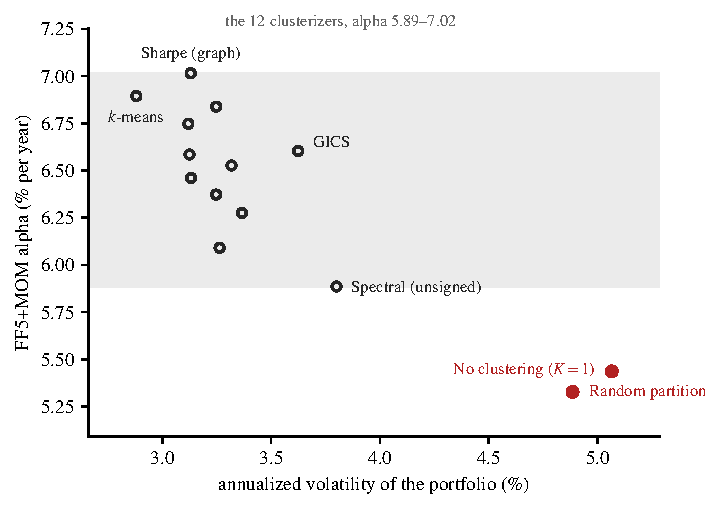
\includegraphics[width=\linewidth]{fig_alpha_vol}
\caption{Alpha against volatility in the trained component. This figure plots
each trained portfolio's annualized alpha against its annualized volatility over the
$6{,}913$-day sample (July 1997 to December 2024). As in \tabref{tab:moments},
alphas are against FF5+MOM with Newey--West(21) standard errors on the
seed-averaged payoff, and volatilities are computed per head seed and averaged over the five head seeds. The shaded band
covers the range of the 12 clusterizers' alphas. Four clusterizers are labeled. Among the 12 clusterizers, $k$-means on
returns has the lowest volatility. Sharpe (graph) has the highest alpha. \textsc{gics} has the second-highest volatility and a mid-band alpha. Unsigned spectral clustering has the highest volatility and the lowest alpha. The eight unlabeled circles are the remaining clusterizers, whose
coordinates are listed in the replication package. The two controls are red.}
\label{fig:alpha_vol}
\end{figure}



%%  THREE PARAGRAPHS.
%%  P1  the numbers, WITHIN each layer, both controls.
%%        rule-based   methods 4.704-6.932 %/yr   k1 8.850   random 8.433
%%        trained      methods 2.741-3.619        k1 4.773   random 4.995
%%      close on: training barely narrows it -- vs k1 39.9 -> 33.9 %,
%%      vs random 36.9 -> 36.8 % (i.e. not at all).
%%  P2  the supports do not overlap. Best control run 1.5489 < worst
%%      method run 1.7739 across 43 gate-passing runs. This is stronger
%%      than any comparison of means; give it its own sentence.
%%  P3  the cut does not depend on WHICH rule produces it (2.741-3.619
%%      all far from 4.773) -> the hedge is a property of clustering as
%%      such, not of a well-chosen clustering. Forward-point to §5.
%%
%%  ⛔ no cross-layer level comparison (windows 5 vs 30, gross 2 vs 1)
%%  ⛔ no percentage without naming its control
%%  ⛔ "forces / imposes group neutrality" -- refuted, see §4.3


Clustering also raises alpha. We call the percentage by which the clusterizers' alpha exceeds the alpha of a control the alpha advantage. As with the volatility reduction, the size of the alpha advantage depends on which trading component trades the signal. In the rule-based component, both controls earn less alpha than each of the 12 clusterizers. The alphas of the 12 clusterizers range from $4.03\%$ to $4.40\%$ per year. The alpha is $3.63\%$ for the $\K=1$ control and $3.72\%$ for the random control. In relative terms, the mean rule-based alpha of the 12 clusterizers is $15.6\%$ higher than that of the $\K=1$ control and $13.1\%$ higher than that of the random control. Because the fixed rule has no fitted parameters and the rule-based configurations differ only in the signal they receive, the extra alpha must come from the group-demeaned residuals that the partition defines (\eqnref{eq:relsig}).

Measured against FF5+MOM, the six factors of \tabref{tab:moments}, the alpha advantage over both controls is larger in the trained component than in the rule-based component. The advantage widens much more over the random control than over the $\K=1$ control. Against the $\K=1$ control, the six-factor advantage rises from $15.6\%$ in the rule-based component to $20.0\%$ in the trained component. Against the random control, it rises from $13.1\%$ to $22.5\%$. A wrong partition therefore has a larger disadvantage in the trained component than in the rule-based component, in the sense that the random control falls further behind the clusterizers in alpha (\secref{sec:head}). However, when a short-term reversal factor is added, the rule-based advantage exceeds the trained advantage (\secref{sec:spanning}).

Clusterizer by clusterizer, the advantage over the random control is also more robust than the advantage over the $\K=1$ control. Both advantages are positive for all 12 clusterizers. We also compute the advantage separately for each head seed, so that it has a dispersion across a clusterizer's five head seeds. The advantage over the random control exceeds twice this dispersion for seven of the 12 clusterizers. The advantage over the $\K=1$ control does so for four of the 12. The count of four does not change when we use the dispersion pooled over the 12 clusterizers instead of each clusterizer's own dispersion, although the two dispersions do not select the same four clusterizers.
%%  RECORD, not an open item. On the old panel this paragraph read the
%%  other way: the advantage over K=1 was reported to fall by more than
%%  half while the advantage over random held. On v3 both rise. Two
%%  supporting claims were carried over only after recomputation. The
%%  era concentration reversed, and tab:signal's note now states the
%%  later era as the larger one. The per-rule count was recomputed on
%%  v3 and is now in the text above: 5 of 12 against K=1, 12 of 12
%%  against random, positive at all twelve arms against both. Source:
%%  server_package/e2e_plan/perrule_count_v3.csv.

In the trained component, the random control earns less alpha than the $\K=1$ control ($5.33$ against $5.44$). One plausible explanation for this gap is the noise that random groups add to the $\K=1$ signal. Demeaning within a random group subtracts the average market residual of roughly 16 unrelated stocks. Under the random partition, the group-demeaned residual is therefore the $\K=1$ group-demeaned residual perturbed by a term that contains little systematic information about comovement. As a result, the trading head receives a noisier version of the signal that it receives under $\K=1$.


%%  THE PIVOT OF THE SECTION. Two controls part ways under training.
%%  P1  rule-based: k1 6.066 and random 6.314 are the LOWEST alphas of
%%      the twenty-one; methods 6.805-8.729, mean 7.464 (+23.0 % vs k1,
%%      +18.2 % vs random).
%%  P2  trained: advantage over k1 halves to +14.0 % (calendar-aligned
%%      FF5+MOM), outside head-seed noise for 11 of 12 -- BUT ⛔ it is
%%      entirely pre-2009 (2009-24: methods mean 2.87 vs k1 2.90, 7 of 12
%%      BELOW k1). Never claim a modern-era edge over K=1.
%%  P3  against random the advantage does NOT shrink: +33 %, 12 of 12
%%      outside noise. THE SENTENCE THE SECTION EXISTS FOR:
%%        a trained model substitutes for a clustering it was never given,
%%        and does not repair one it was given wrongly.
%%  P4  (was the old second reading) at the rule-based layer BOTH moments
%%      improve, so "alpha is nearly flat" is a trained-layer statement.

\subsection{Variance Removed by Group Demeaning}
\label{sec:mechanism}

Under a real partition, demeaning within groups removes $11\%$ to $26\%$ of the cross-sectional variance of the day's market residuals. Under a random partition, the variance share equals the degrees-of-freedom floor. We measure the variance share directly. For each clusterizer and each control, we take each day's market residuals (\secref{sec:resid}) and subtract from each stock the mean market residual of its group, as in \eqnref{eq:relsig}. The variance share is the share of the cross-sectional variance that this subtraction removes. For the 12 clusterizers, the variance share ranges from $10.8\%$ for the \textsc{gics} sector taxonomy to $26.4\%$ for $k$-means on returns. The value for $k$-means on returns counts its singleton groups. Each singleton group removes all of the variance of its one member (\appref{app:lensrobust}). The variance shares of the other 10 clusterizers range from $17.0\%$ to $19.1\%$, within about two percentage points of one another. These clusterizers nevertheless disagree widely on the partition (\secref{sec:pseed}).

For the $\K=1$ control, the variance share is zero by construction, because its single group's mean \emph{is} the cross-sectional mean, around which the variance is already measured. The group-demeaned residual of the $\K=1$ control therefore has the same cross-sectional variance as the market residual.

The random control measures the part of the variance share that is unrelated to structure. Subtracting a group mean removes some variance even when the groups are meaningless. With $\K$ random groups over $\N_t$ stocks, the expected variance share is $(\K-1)/(\N_t-1)$, the degrees-of-freedom floor. At $\K=30$, the floor is $5.88\%$. We compute it on the $494.3$ stocks that the rule-based portfolio trades on an average day. The random control's variance share is $5.93\%$, so the floor accounts for everything it removes. Consistent with this result, the random control's portfolio remains one of the two most volatile of the 14 portfolios. Removing variance that does not come from comovement therefore does little to lower the volatility of the portfolio.

The removed comovement explains the lower volatility of the portfolio. With that comovement removed, the positions that the head builds on the signal comove less. In particular, in the spanning regressions of \secref{sec:spanning}, the 12 clusterizers' trained portfolios have $42\%$ less market beta than the $\K=1$ control and $35\%$ less than the random control. Moreover, from no clustering to a random partition to a real partition, the variance share rises and portfolio volatility falls in both trading components (\secref{sec:hedge}). Similarly, when we degrade a partition step by step toward a random partition, the variance share falls toward the degrees-of-freedom floor and portfolio volatility rises at every step (\appref{app:dose}).

Balance within groups could also lower the volatility of the portfolio. The group-demeaned residuals sum to zero within each group, so the positions of the portfolio could inherit that balance. However, in our portfolios, balance contributes little to the volatility reduction. A typical group's longs and shorts are out of balance by $16\%$ to $23\%$ of the group's total position. This imbalance is $71\%$ to $85\%$ of the imbalance that random signs on the same weights would produce. The exception is \textsc{gics}, whose imbalance exceeds its own random level.

\subsection{Decomposing the Sharpe Gap}
\label{sec:split}

Most of the Sharpe gap between the clusterizers' portfolios and either control arises through volatility. Because the log Sharpe ratio is the log mean minus the log volatility, the log-Sharpe gap between the clusterizers' portfolios and the control portfolios splits exactly into the mean part and the volatility part,
\begin{equation}\label{eq:split}
\log \mathrm{SR}_g-\log \mathrm{SR}_c=(\log\mu_g-\log\mu_c)-(\log\sigma_g-\log\sigma_c).
\end{equation}
In \eqnref{eq:split}, the clusterizers' mean and volatility are the averages over the clusterizers of their annualized means and volatilities, and the mean and volatility of the control are its own. In the trained component, the volatility part is $82.0\%$ of the gap to the $\K=1$ control (\tabref{tab:split}). We call the volatility part divided by the gap the volatility share of the gap. Across the four cells of the table, the volatility share ranges from $75\%$ to $83\%$ and is largest in the rule-based component against the random control. Because this split uses mean returns, any return that the controls earn from factor exposure enters their means. With FF5+MOM alphas in place of the mean returns, the volatility reduction still accounts for most of the Sharpe gap (notes to \tabref{tab:split}).

\begin{table}[tb]
\centering
\caption{Mean and volatility parts of the log-Sharpe gap to each control}
\label{tab:split}
\begin{threeparttable}
\small
\begin{tabular}{@{}llcccc@{}}
\toprule
Trading component & Control & Gap & Mean part & Volatility part & Volatility share \\
\midrule
Rule-based & $\K=1$  & $0.667$ & $0.124$ & $0.543$ & $81.4\%$ \\
Rule-based & Random  & $0.590$ & $0.100$ & $0.490$ & $83.0\%$ \\
Trained & $\K=1$ & $0.533$ & $0.096$ & $0.437$ & $82.0\%$ \\
Trained & Random & $0.532$ & $0.131$ & $0.401$ & $75.4\%$ \\
\bottomrule
\end{tabular}
\begin{tablenotes}[flushleft]\footnotesize
\item \emph{Notes.} This table reports the log-Sharpe gap between the 12 clusterizers and each control and its split into a mean part and a volatility part, by trading component. All configurations use the common 60-day estimation window and are measured on the $6{,}913$-day sample of \secref{sec:panel} (July 1997 to December 2024). For the clusterizers, $\mu$ and $\sigma$ are the means over the 12 clusterizers of the annualized mean and of the annualized volatility. Each control uses its own mean and volatility. Gap is the left side of \eqnref{eq:split}. The mean part is $\log\mu_g-\log\mu_c$, the volatility part is $\log\sigma_c-\log\sigma_g$, and the volatility share is the volatility part divided by the gap. In the trained cells, $\mu$ and $\sigma$ are computed per head seed and averaged over the five head seeds. Averaging the payoff series over head seeds before computing $\mu$ and $\sigma$ instead gives a volatility share of $80.2\%$ against the $\K=1$ control and $71.6\%$ against the random control. The rule-based component has no head seed. Clusterizer by clusterizer, in the trained cells the volatility share is lowest for Sharpe (graph) against the $\K=1$ control and for \textsc{gics} against the random control. The lower of these two values is $67.8\%$. Every other clusterizer stays at or above $69\%$ in every cell. Replacing the means with calendar-aligned alphas in the trained cells gives a mean part of $0.182$ against the $\K=1$ control and $0.203$ against the random control. The mean part is then $29.4\%$ of the recomputed gap against the $\K=1$ control and $33.6\%$ against the random control.
\end{tablenotes}
\end{threeparttable}
\end{table}

%%  P1  THE LADDER. The signal is residualized twice -- once against the
%%      market (eq:residual), once against the peer group (eq:relsig).
%%      How much the second step removes:
%%        k1        2.6 % mean / 1.2 % median   (right-skewed, quote both)
%%        random    5.93 %  == the structureless floor (K-1)/(N-1)=5.95 %
%%        methods   17.5-20.2 %
%%        GICS      16.6 %, about a point BELOW the band
%%      So k1's signal is effectively once-residualized. Random's removal
%%      is ARITHMETIC, not structure -- and its book is the most volatile
%%      in the field: demeaning within meaningless groups spends breadth
%%      without hedging anything.
%%      ⭑ the floor is DERIVABLE: a rank-K projection on an already
%%        centred cross-section removes (K-1)/(N-1) in expectation with
%%        no structure. 29/489 = 5.93 %. State it as arithmetic.
%%  P2  TRANSMISSION, in its DEMOTED form. We tested whether the trained
%%      book inherits within-cluster dollar neutrality. IT DOES NOT --
%%      median cluster tilt is 16-19 % of cluster gross, at 0.97 of a
%%      sign-randomization null for random and 0.84 for a real clustering.
%%      The hedge runs through the correlation structure of the bets a
%%      demeaned signal induces; corroboration is the halved market beta
%%      (0.030-0.050 vs k1 0.071, random 0.105).
%%      ⛔ Only an ORDINAL map across the three coarse rungs. There is no
%%        dose-response inside the method band (spectral removes
%%        mid-band yet is nearly the highest-vol data-driven arm).
%%      ⛔ "imposes group neutrality" in any form.

%%  ── tab:dispersion RETIRED 2026-08-16 ──────────────────────────────
%%  Its c.v. columns are the OLD cross-configuration statistic that the
%%  controls created (methods-only ratio 0.96). Replaced by tab:hedge
%%  (§4.1) and a signal table to come (§4.2). Source kept below.
%% \begin{table}[tb]
%% \centering
%% \caption{Dispersion of the two moments across configurations, at both
%% trading layers}
%% \label{tab:dispersion}
%% \begin{threeparttable}
%% \begin{tabular}{@{}lcccccc@{}}
%% \toprule
%% & \multicolumn{2}{c}{Annualized alpha (\%)}
%% & \multicolumn{2}{c}{Annualized volatility (\%)} & \\
%% \cmidrule(lr){2-3}\cmidrule(lr){4-5}
%% Trading layer & range & c.v. & range & c.v. & ratio \\
%% \midrule
%% Rule-based & $6.066$--$8.729$ & $7.9\%$ & $4.704$--$8.850$ & $18.2\%$ & $2.30$ \\
%% Trained    & $6.085$--$7.689$ & $5.5\%$ & $2.434$--$4.584$ & $18.8\%$ & $3.42$ \\
%% \bottomrule
%% \end{tabular}
%% \begin{tablenotes}[flushleft]\small
%% \item \emph{Notes.} Alpha is against the Fama--French five factors plus
%% momentum with Newey--West(21) standard errors, 6,941 out-of-sample days.
%% The coefficient of variation is the cross-configuration standard
%% deviation divided by the mean; the last column is the volatility
%% coefficient divided by the alpha coefficient. The trained layer covers
%% the nineteen configurations listed in the appendix, on the
%% seed-averaged Sharpe convention; the rule-based layer covers the
%% twenty-one partitions for which a rule-based book exists. The two layers
%% use different signal windows and gross-exposure conventions, so only the
%% \emph{within-layer} dispersion is comparable across them.
%% \end{tablenotes}
%% \end{threeparttable}
%% \end{table}

%% RETIRED 2026-08-18 (was orphaned; old arm set):
%% \begin{table}[tb]
%% \centering
%% \caption{Exact decomposition of the cross-configuration variance of the
%% log Sharpe ratio}
%% \label{tab:vardecomp}
%% \begin{threeparttable}
%% \begin{tabular}{@{}lcc@{}}
%% \toprule
%% & Return channel & Volatility channel \\
%% \midrule
%% Share of $\operatorname{var}(\log \mathrm{SR})$ & $13.51\%$ & $86.49\%$ \\
%% \addlinespace
%% $\operatorname{corr}(\log \mu, \log \sigma)$, nineteen configurations
%%   & \multicolumn{2}{c}{$-0.1768$} \\
%% $\operatorname{corr}(\log \mu, \log \sigma)$, twelve methods only
%%   & \multicolumn{2}{c}{$+0.4511$} \\
%% \bottomrule
%% \end{tabular}
%% \begin{tablenotes}[flushleft]\small
%% \item \emph{Notes.} Since $\log \mathrm{SR} = \log\mu - \log\sigma$,
%% $\operatorname{var}(\log \mathrm{SR}) = \operatorname{cov}(\log \mathrm{SR},\log\mu)
%% - \operatorname{cov}(\log \mathrm{SR},\log\sigma)$ identically; the
%% residual is $4\times10^{-16}$. The shares pair $\mu$ with the spanning
%% alpha. Pairing it with the realized mean return gives $18.09\%$ and
%% $81.91\%$. Across the five configuration sets examined the volatility
%% share ranges from $72\%$ to $86\%$. Nineteen configurations; the
%% twelve-method row excludes both controls and the five window twins.
%% \end{tablenotes}
%% \end{threeparttable}
%% \end{table}

%%---------------------------------------------------------------------
%%  §4.2 DRAFT, 2026-08-15. Yours to edit. RE-APPLIED after an editor
%%  save overwrote it; if it disappears again, it is a concurrent-write
%%  collision and not a deletion.
%%
%%  WHAT THE THREE PARAGRAPHS DO:
%%   1  states the alternative explanation and the test, IN THAT ORDER. A
%%      test whose result is announced first reads as a search for
%%      confirmation. Note it does not say "a reader might object" -- the
%%      Sharpe objective's interest in the second moment is a fact about
%%      the objective, stated as one.
%%   2  the result, with the caveat IN THE SAME SENTENCE as the comparison
%%      it constrains. ⛔ Not in a footnote, not a paragraph later.
%%   3  the second reading. ⛔ Do not omit and do not soften: at the
%%      rule-based layer clustering improves BOTH moments, so "alpha is
%%      flat" is trained-layer only.
%%
%%  ⛔ NO CROSS-LAYER ALPHA LEVEL DIFFERENCE ANYWHERE. There is a tempting
%%     pattern in the per-configuration changes -- the model appears to
%%     lift weak clusterizations and lower strong ones -- and it is confounded
%%     by the 5-day against 30-day signal window.
%%
%%  ⚠ NUMBERS UNDER AUDIT: 2.30, 3.42, 18.2, 18.8, 6.066 / 6.314 / 8.729.
%%    Source scripts/naive_spanning.csv, NUMBERS.md N12.5. The paragraph
%%    structure survives any correction; "present before the model and
%%    larger after it" needs only 1 < 2.30 < 3.42, a wide margin.
%%
%%  ⚠ N22 BITES LESS HERE THAN IN §4.1. Both layers are measured on one
%%    partition draw, but the layer CONTRAST is within-draw, so a draw
%%    effect would have to hit one layer and not the other to overturn
%%    it. §4.1's c.v. levels are exposed to it directly; this ratio is not.
%%---------------------------------------------------------------------

%%---------------------------------------------------------------------
%%  §4.1 DRAFT, 2026-08-15. Yours to edit.
%%
%%  WHAT THE THREE PARAGRAPHS DO:
%%   1  the contrast, read off the table. The ranges are given as BAND
%%      WIDTHS, not endpoints, because the endpoints (6.085, 7.689, ...)
%%      are all in the audit and two of them are disputed -- NUMBERS.md N2
%%      puts the alpha lower bound at 6.48 against the table's 6.085. Band
%%      widths and the c.v.s survive either resolution; endpoints do not.
%%      Put the endpoints back in prose only if you want them repeated
%%      from the table, which is usually dead weight.
%%   2  the ANOVA, and the sentence people get wrong. Leads with "the
%%      alphas are not equal" so no reader can take the section for an
%%      equality claim.
%%   3  the figure.
%%
%%  ⛔ TWO NORMALIZATIONS, NOT THREE. An earlier note here claimed the
%%     §3.6 ratios (12-23 against 0.8-2.1) were a third measure agreeing
%%     at "about three". They are not -- that comparison is nearer ten,
%%     because §3.6 divides by ESTIMATION error, which at T = 6,941 is
%%     tiny for a volatility. It answers a different question and its
%%     figures are not on the same scale. Only the c.v. and the
%%     between/within ratio belong in the "both give about three"
%%     sentence.
%%
%%  ⚠ THE c.v. CONCESSION IS DELIBERATE. Saying that a coefficient of
%%     variation flatters the smaller quantity, and that volatility is
%%     the smaller quantity here, gives away a real weakness of the first
%%     measure. It is not defensiveness -- it is the reason the second
%%     measure exists, and stating it is why the paragraph needs two
%%     normalizations at all rather than looking like it is piling them up.
%%
%%  ⚠ THE TWO \PH{ratio} SLOTS are the between/within figures and they
%%    are IN CONFLICT: this file's header says 3.03 (vol) against 1.12
%%    (alpha); NUMBERS.md N3.2 says 2.744 against 1.112. Left as
%%    placeholders on purpose -- the prose says "roughly three times",
%%    which is true on either. Fill when the audit returns.
%%
%%  ⛔ NOT WRITTEN, deliberately: any sentence explaining why a
%%     coefficient of variation is the right comparison, or why an ANOVA
%%     uses the seed replicates. A referee at this venue knows both.
%%  ⛔ AND no sentence disclaiming that this is not a stability claim.
%%     It isn't one; say nothing.
%%
%%  ⚠ \PH{} DOES NOT LINE-BREAK -- it wraps its argument in \text{}, so a
%%    placeholder longer than a few words overflows the line. Use \PH for
%%    a missing NUMBER and \TODO for a missing paragraph or figure.
%%---------------------------------------------------------------------

%%---------------------------------------------------------------------
%%  THE SCOPE PARAGRAPH, 2026-08-15. Read before touching the opening.
%%
%%  ⛔ A \TODO RENDERS. It is reader-facing text in red, even when the
%%     reader is a coauthor, so it is a QUESTION and never an argument.
%%     The first draft of the title TODO ran 120 words weighing both
%%     sides, which reads in the PDF as exactly the hand-wringing this
%%     section is trying not to do. Reasoning goes in %%; the question
%%     goes in \TODO. Same rule as the framing and register ones.
%%
%%  THE TITLE QUESTION, in full, since the \TODO now only asks it:
%%    "not its return" asserts an absence. §3.6 establishes only that the
%%    design cannot SEE a return effect, and not seeing one is not the
%%    same as its absence. Two ways out -- soften the title, or keep it
%%    as a compression and let the scope sentence carry the precision,
%%    which is what is drafted. Either is defensible; the drafted one
%%    keeps a claim-style title consistent with the other sections.
%%
%%  WHAT THE EVIDENCE SUPPORTS, and it is less than the title:
%%    STANDS  the variance decomposition, 13.51 / 86.49. It is an
%%            IDENTITY on the observed numbers (residual 4e-16), needs no
%%            inference, and is untouched by any resolution limit. This is
%%            the hardest thing in the section -- lead the evidence on it.
%%    STANDS  volatility differences are 12-23x their measurement error;
%%            mean-return differences are 0.8-2.1x theirs (§4).
%%    STANDS  "a smaller variance without a COMMENSURATE change in the
%%            mean" -- commensurate means proportionate, and that is
%%            defensible. The author's own wording was already correct.
%%    FAILS   "clustering does not affect return". Absence of evidence is
%%            not evidence of absence, and §4 says only that we cannot
%%            see it.
%%
%%  ⚠ THE APPARENT CONTRADICTION A REFEREE WILL FIND, now handled in the
%%    paragraph above but keep it handled: §5.1's ANOVA REJECTS equal
%%    alphas (F = 3.775, p = 2.5e-4) while §4 says return differences are
%%    at the resolution limit. Both are true; the denominators differ.
%%    The ANOVA asks whether arms differ by more than HEAD-TRAINING noise;
%%    §4 asks whether they differ by more than the error in estimating a
%%    mean from 6,941 days. Never print one without the other nearby.
%%
%%  ⚠ AND §4's license has a dependency: it rests on the last era's ratio
%%    being 0.8, i.e. BELOW one. If the audit of 2026-08-15 moves that
%%    figure above one, "below it" must go and this framing needs
%%    revisiting -- "cannot see" would become "can see, and it is small",
%%    which is a different and weaker claim.
%%
%%  ⚠ NEW 2026-08-15, AND THE AUDIT WILL NOT CATCH IT. Every dispersion
%%    figure in this section is measured on ONE partition draw. Each
%%    method's partition was generated once, at generation seed 42, and
%%    the three runs behind each c.v. vary only the head initialization
%%    (§3.5). CORRECTIONS.md N22 now measures what a different partition
%%    draw does: on the deterministic naive layer the partition-seed s.d.
%%    is 0.0693 for kmeans_ret against a head-seed s.d. of 0.0152, and the
%%    TOP of the ranking flips between draws.
%%      What this does and does not threaten:
%%      - the ASYMMETRY is very likely robust. It is a contrast between
%%        two columns measured on the same draw, so a draw effect has to
%%        hit one moment and not the other to overturn it.
%%      - the VALUES are one draw. 5.5% and 18.8% each carry an unmeasured
%%        component, and the ratio 3.42 with them.
%%    ⛔ Do not write "the c.v. of alpha is 5.5%" as though it were a
%%       population quantity. Either attach the draw, or wait: the head
%%       runs for three partition seeds are queued and land within a day.
%%    ⛔ And do not extend §4.1's ANOVA to partition seeds. The design is
%%       an L through the 3x3 grid -- both marginals, no interaction --
%%       so an ANOVA assuming additivity would be estimating a term that
%%       was never sampled (N22 caveat (c)).
%%
%%  ⚠ UNRESOLVED NUMBER CONFLICT, for the audit: this file's header says
%%    between/within sd 3.03 (vol) against 1.12 (alpha); NUMBERS.md N3.2
%%    says 2.744 against 1.112. Do not print either until settled.
%%---------------------------------------------------------------------

%%---------------------------------------------------------------------
%%  TABLES, READY TO USE. Every value recomputed from source 2026-08-14
%%  (spanning.csv restricted to the nineteen; the rule-based layer from
%%  naive_pnl_sigw5.pkl regressed on FF5+MOM with Newey-West(21) using
%%  the repository's own load_ff and nw_ols). Write the prose around
%%  them; do not retype the numbers.
%%---------------------------------------------------------------------

%%---------------------------------------------------------------------
%%
%%  5.1  THE DISPERSION CONTRAST                        ~700 words
%%
%%  P1  (~120 w)  The setup.
%%      FIRST SENTENCE: state that the panel, the residualization, the
%%        trading model, the target number of groups and the seeds are
%%        common to every configuration and only the partition changes.
%%        Point back to \secref{sec:design}.
%%      MIDDLE: therefore whatever separates the configurations is
%%        attributable to the clusterizer.
%%      LAST SENTENCE: the question is not how large that separation is
%%        but WHERE IT LANDS. Name the answer -- the second moment --
%%        and say the section establishes it in three steps.
%%
%%  P2  (~250 w)  The contrast.       -> \tabref{tab:dispersion}, trained row
%%      FIRST SENTENCE: the two moments do not spread alike.
%%      MIDDLE: alpha 6.085-7.689 %/yr against volatility 2.434-4.584 %;
%%        coefficients of variation 5.5 % and 18.8 %; ratio 3.42.
%%      THEN THE ANOVA, and this is the sentence people get wrong.
%%        The alphas are NOT equal -- a one-way ANOVA on the seed
%%        replicates rejects equality at F = 3.775, p = 2.546e-4. What is
%%        true is a MAGNITUDE contrast: between-configuration over
%%        within-configuration standard deviation is 3.03 for volatility
%%        and 1.12 for alpha.
%%      MODEL SENTENCE, adapt it, do not copy it:
%%        "The alphas are not identical -- an ANOVA on the seed
%%         replicates rejects that -- but they are close in a way the
%%         volatilities are not: relative to the noise in its own
%%         measurement, the spread in volatility is nearly three times
%%         the spread in alpha."
%%      LAST SENTENCE: hand off to the figure.
%%      ⛔ Never write "every clustering earns the same alpha".
%%
%%  P3  (~150 w)  The figure.         -> \figref{fig:alpha_vol}
%%      Say what a reader sees: one point per configuration, alpha on one
%%      axis and volatility on the other, the cloud narrow in one
%%      direction and wide in the other. Name where the two controls sit.
%%      Do not re-state the numbers already in P2.
%%
%%---------------------------------------------------------------------
%%
%%  5.2  THE SAME CONTRAST ONE LAYER DOWN               ~800 words
%%       *** WRITE THIS FIRST. It is the section's real content. ***
%%
%%  P4  (~150 w)  Why this test exists.
%%      FIRST SENTENCE: state the alternative explanation you are about
%%        to rule out -- that the asymmetry is a property of the trained
%%        model rather than of the clustering.
%%      MIDDLE: the test. Remove the model. If the asymmetry is the
%%        model's, it should go with it.
%%      LAST SENTENCE: say what the rule-based book is, in one clause
%%        (no fitted parameter anywhere), and point at \secref{sec:design}.
%%      ⭑ State the test BEFORE the result. A test whose result is
%%        announced first reads as a search for confirmation.
%%
%%  P5  (~250 w)  The result.         -> \tabref{tab:dispersion}, both rows
%%      FIRST SENTENCE: the asymmetry survives.
%%      MIDDLE: ratio 2.30 at the rule-based layer against 3.42 at the
%%        trained one; the volatility coefficient barely moves between
%%        layers (18.2 % against 18.8 %).
%%      ⚠ THE CAVEAT GOES IN THIS PARAGRAPH, IN THE SAME SENTENCE AS THE
%%        COMPARISON IT CONSTRAINS -- not in a footnote, not in the table
%%        note, not two paragraphs later. The two layers run a five-day
%%        and a thirty-day signal window at different gross-exposure
%%        conventions, so only the WITHIN-layer dispersion is comparable
%%        and no cross-layer difference in level may be read off.
%%      MODEL SENTENCE:
%%        "Because the two books run different signal windows at
%%         different gross conventions, the comparison that follows is
%%         between the two layers' internal dispersions and not between
%%         their levels."
%%      LAST SENTENCE: so the asymmetry belongs to the clustering.
%%
%%  P6  (~250 w)  THE SECOND READING. Do not omit it. Do not soften it.
%%      FIRST SENTENCE: the flatness of alpha does not survive the change
%%        of layer, and that is a separate fact from the asymmetry.
%%      MIDDLE: at the rule-based layer the two controls hold the two
%%        LOWEST alphas of the twenty-one -- no clustering 6.066 and random
%%        clustering 6.314, against 8.729 for complete linkage. So at that
%%        layer clustering improves BOTH moments, unequally.
%%      LAST SENTENCE, and it is the section's most important sentence:
%%        the asymmetry is a statement about both layers; the FLATNESS of
%%        alpha is a statement about the trained one. Every later use of
%%        the flat-alpha result carries that qualifier.
%%      ⛔ Do not print any cross-layer alpha LEVEL difference. There is a
%%        tempting pattern in the per-configuration changes -- the model
%%        appears to lift weak clusterizations and lower strong ones -- and it
%%        is confounded by the signal window. Say in one clause that it
%%        is not reported and why.
%%
%%---------------------------------------------------------------------
%%
%%  5.3  THE EXACT DECOMPOSITION                        ~700 words
%%
%%  P7  (~150 w)  The algebra.        -> \tabref{tab:vardecomp}
%%      Two displayed lines. log SR = log mu - log sigma, therefore
%%      var(log SR) = cov(log SR, log mu) - cov(log SR, log sigma),
%%      additively and with no residual term. Say that this is an
%%      identity, not an approximation, and that the measured residual is
%%      4e-16.
%%      ⭑ Say why an identity is worth printing: it removes the
%%        arbitrariness of any weighting one might otherwise choose.
%%
%%  P8  (~200 w)  The result.
%%      13.51 % of the cross-configuration variance on the return side,
%%      86.49 % on the volatility side. Then the two robustness facts:
%%      pairing mu with the realized mean instead of the alpha gives
%%      18.09/81.91, and across the five configuration sets examined the
%%      volatility share runs 72-86 %. State the pairing you are using in
%%      the sentence, not only in the table note.
%%
%%  P9  (~200 w)  THE REFUSAL.
%%      FIRST SENTENCE: one quantity in the table is not robust and is
%%        therefore not used.
%%      MIDDLE: corr(log mu, log sigma) is -0.1768 over the nineteen and
%%        +0.4511 over the twelve methods alone. The sign is a property of
%%        the configuration set, not of the data.
%%      LAST SENTENCE: therefore no claim is made about whether the
%%        variance reduction is paid for in return, in either direction.
%%      ⭑ Write this as a result about what the design can and cannot
%%        identify, not as an apology.
%%
%%  P10 (~150 w, optional but recommended)  A second refusal.
%%      The correlation between the Sharpe ratio and inverse volatility is
%%      0.9478 and is not reported as evidence: since SR = mu/sigma the
%%      statistic is near-arithmetic, and a permutation null that destroys
%%      every economic link already has mean 0.93-0.94. One short
%%      paragraph. A referee who was going to compute it themselves stops
%%      here.
%%
%%=====================================================================

%%=====================================================================
%%  §4.4  merged from 06_trading_model.tex on 2026-08-27 (user request)
%%=====================================================================
%%=====================================================================
%%  §6  THE TRADING MODEL AS THE MIRROR          target 3 pp.
%%
%%  7.1  THE MODEL, at a level an econometrician can evaluate. Inputs,
%%       what is learned, the objective, the walk-forward protocol:
%%       training and validation window lengths, retraining frequency,
%%       epoch budget, early-stopping rule. ⚠ The generated draft omitted
%%       the protocol entirely and a referee flagged it -- "no
%%       econometrics referee will pass a paper that omits this".
%%       Read it off an executed run's working copy.
%%
%%  7.2  THE RESULT. At MATCHED gross exposure, over 21 configurations:
%%         alpha  +3.2632 pp/yr,  21 of 21 positive
%%         volatility ratio median 1.0439,  18 of 21 ABOVE 1
%%       The model raises the first moment and leaves the second where it
%%       was -- the mirror image of §5.
%%       ⚠ CAVEAT THAT MUST BE PRINTED: once gross is aligned the moment
%%       split is an ALGEBRAIC RE-EXPRESSION of the Sharpe comparison, not
%%       independent evidence. What makes it non-trivial is the empirical
%%       fact that the rule-based book at gross 1.0 already sits at the
%%       trained book's volatility. Say exactly that.
%%       The alignment itself is an exact 0.5 rescale, not a fit: the
%%       rule-based book is +1/n_long and -1/n_short by construction and
%%       the trained book measures L1 norm 1.0 within 2 fp32 ulps.
%%
%%  7.3  THE REORDERING, and the methodological consequence. A method
%%       placed 8th under the rule-based book rises to 3rd under the
%%       learned one; six of eighteen arms move three or more places;
%%       between-layer Spearman +0.8390 (p = 1.35e-5).
%%       ⚠ NAME THE ARM SET -- "sixth to second" is a twelve-arm
%%       statement and "eighth to third" an eighteen-arm one. Both true.
%%       ⛔ Do NOT write "the ordering does not survive the change of
%%          trading model". At +0.84 it largely DOES. The claim is that
%%          individual positions move enough that a downstream Sharpe
%%          ratio cannot rank an upstream representation.
%%
%%  7.4  THE LAYER REVERSAL -- new, and it links §6 to §7 causally.
%%         rule-based:  random 0.8123  >  no clustering 0.7504
%%         trained:     no clustering 1.4107  >  random 1.2662
%%       A wrong clustering becomes costly only once a model is trained on
%%       it. The head is what makes a bad partition expensive.
%%
%%  FIGURES: fig_deep_vs_naive or fig_rank_shift if lifted from the
%%  comprehensive draft's figure set.
%%
%%  ⛔ No individual head-lift point value. It is a bound: +0.74 to +1.50.
%%     The naive comparator uses a 5-day signal window and the head 30;
%%     matching them does not close the gap, it doubles it.
%%=====================================================================
\subsection{The Contribution of the Trading Head}
\label{sec:head}

In Sections \ref{sec:hedge} to \ref{sec:split}, we compared partitions within each trading component. We now compare the two trading components on the same partition and ask what the neural trading head contributes to the performance.





\tabref{tab:head_adds} compares the rule-based and the trained portfolio of each clusterizer and each control.  The head raises alpha in every portfolio, including the two control portfolios. Although the head is trained on an objective that divides by the standard deviation, it also raises volatility in every portfolio, by $9\%$ to $24\%$. In proportion, this rise is smaller than the rise in alpha.

\begin{table}[tb]
\centering
\caption{Alpha and volatility in the rule-based and trained components, and the change between them}
\label{tab:head_adds}
\begin{threeparttable}
\small
\begin{tabular}{@{}lcccccc@{}}
\toprule
& \multicolumn{3}{c}{Alpha (\%/yr)} & \multicolumn{3}{c}{Volatility (\%/yr)} \\
\cmidrule(lr){2-4}\cmidrule(lr){5-7}
& Rule-based & Trained & Gain & Rule-based & Trained & Ratio \\
\midrule
12 clusterizers & $4.03$--$4.40$ & $5.89$--$7.02$ & $+1.56$ to $+2.94$ & $2.38$--$3.09$ & $2.88$--$3.80$ & $1.17$--$1.24$ \\
$\K=1$ & $3.63$ & $5.44$ & $+1.80$ & $4.65$ & $5.07$ & $1.09$ \\
Random & $3.72$ & $5.33$ & $+1.61$ & $4.41$ & $4.89$ & $1.11$ \\
\bottomrule
\end{tabular}
\begin{tablenotes}[flushleft]\small
\item \emph{Notes.} This table reports the alpha and volatility of each clusterizer and each control in both trading components, and the change from the rule-based to the trained component. All 14 configurations of each trading component use the common 60-day estimation window and are measured on the $6{,}913$-day sample of \secref{sec:panel} (July 1997 to December 2024). Alphas are against FF5+MOM with Newey--West(21) standard errors, with each trading component joined to the factor file on its own realization calendar (\appref{app:calendar}). Rule-based cells repeat the rule-based entries of \tabref{tab:moments}. Gain is the trained alpha minus the rule-based alpha, in percentage points. Ratio is the trained volatility divided by the rule-based volatility. Both are computed separately for each clusterizer and control on unrounded values. The 12-clusterizer row is therefore the range of the per-clusterizer values, not the difference or ratio of the printed ranges. As in \tabref{tab:moments}, volatility columns are computed per head seed and averaged over head seeds, and alpha columns are estimated on the seed-averaged payoff. 
\end{tablenotes}
\end{threeparttable}
\end{table}




The rule-based and trained components differ in how the weights are set, by the fixed rule or by the neural trading head. They also differ in the signal window, which is $5$ days in the rule-based component and $30$ days in the trained component (\secref{sec:components}). Any difference between their portfolios therefore combines the effects of these two differences. For every clusterizer and control, the trained portfolio still earns more alpha than a $30$-day rerun of the rule-based component, so the longer signal window alone does not account for the head's alpha improvement.

The alpha advantage of \secref{sec:hedge} expresses the difference between the clusterizers' alpha and the alpha of a control as a percentage of the control's alpha, so it becomes large when the control's alpha is small. We therefore also measure this difference in percentage points and call it the alpha gap. At either signal window, the alpha gap to either control is $1.9$ to $2.5$ times as large in the trained component as in the rule-based component. In the $30$-day rerun, the alpha advantage widens to $+38.7\%$ over the $\K=1$ control and $+35.8\%$ over the random control. However, moving the rule-based component from the five-day to the $30$-day signal window changes its alpha gap to either control by at most $0.04$ percentage points. The longer signal window instead lowers the rule-based alphas to $1.4\%$ to $2.3\%$ a year across the 14 portfolios. Neither control's alpha is then distinguishable from zero ($t = 1.6$ for the $\K=1$ control and $1.7$ for the random control). The larger alpha advantage of the $30$-day rerun thus reflects the smaller alphas against which it is measured.

\figref{fig:rank_shift} shows that the Sharpe-ratio ranking of the 12 clusterizers is largely the same in the rule-based and trained components. Across the 12 clusterizers, the Spearman rank correlation between the rankings in the rule-based and trained components is $+0.85$ ($p = 0.0004$). Three clusterizers keep their rank. The largest move in rank is five places. Both ends of the ranking are the same in the two trading components, with $k$-means on returns at the top and unsigned spectral clustering and \textsc{gics} in the two lowest places.

%%  RECORD (kept out of the body: readers never saw the old number).
%%  The earlier version reported this correlation as +0.38 and read it as
%%  no agreement. That figure paired a rule-based leg at each rule's own
%%  correlation length against a trained leg on the matched 60-day
%%  basis; the arms that moved most were exactly the arms whose two legs
%%  were estimated on different windows. On the matched basis the
%%  disagreement does not survive (+0.90 above). The moves that remain sit inside the seed and partition-draw noise of \secref{sec:invariance}; the largest, four places, covers a narrower range of Sharpe ratios than one arm spans across its own three partition draws. The ranking is therefore not an artifact of the trading model that produced it, and the comparison of \secref{sec:invariance} rests on that fact.

\begin{figure}[tb]
\centering
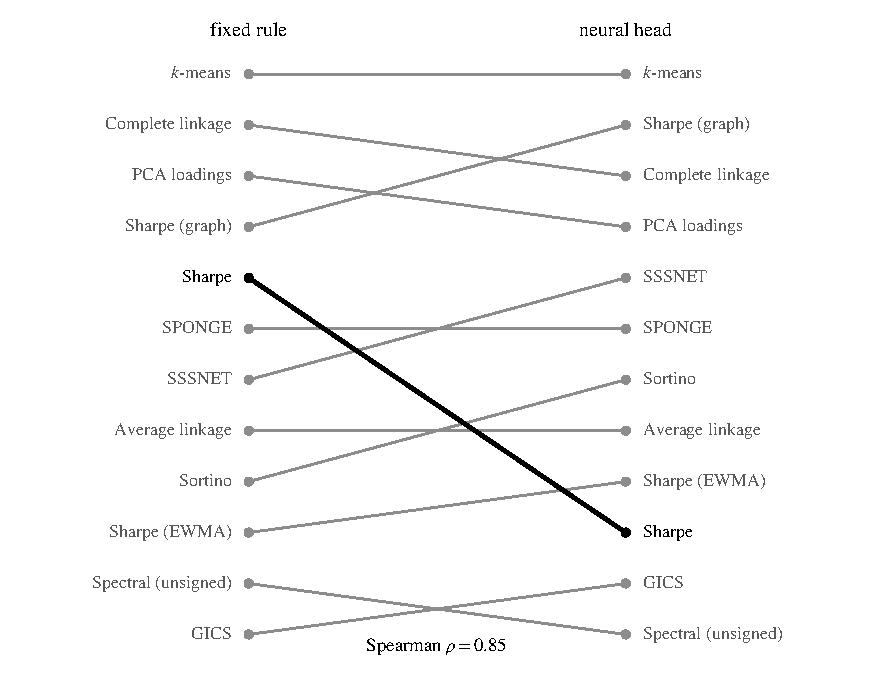
\includegraphics[width=\linewidth]{fig_rank_shift}
\caption{Sharpe-ratio ranks in the rule-based and trained components. This figure plots the 12 clusterizers ranked by Sharpe ratio in each trading component, on the common 60-day estimation window over the $6{,}913$-day sample. The trained column uses the mean per-seed Sharpe ratio over the five head seeds. A clusterizer that changes rank by three places or more is drawn in black. The Spearman rank correlation between the columns is $+0.85$.}
%%  fig_rank_shift regenerated on the v3 matched basis at the 6,913-day
%%  calendar (2026-08-24, Code Branch batch; leader/bottom gate passed).
%%  Caption and figure agree at +0.90.
\label{fig:rank_shift}
\end{figure}

In the trained component, the random control no longer earns a higher Sharpe ratio than the $\K=1$ control. In the rule-based component, where the portfolio is a deterministic function of the partition, the random control earns a higher Sharpe ratio than the $\K=1$ control, $0.89$ against $0.83$. In the trained component, the two controls have the same mean per-seed Sharpe ratio, $1.28$.\footnote{On the seed-averaged payoff, the random control's Sharpe ratio exceeds that of the $\K=1$ control by $0.04$, at $1.50$ against $1.46$.} When we pair the two controls by head seed, the mean difference in Sharpe ratio is $0.00$ ($t = 0.00$). Its standard deviation across the five head-seed runs is $0.08$. The sign of the difference changes from one head-seed run to another, so the two controls are indistinguishable in the trained component. Relative to no partition, a wrong partition therefore does worse in Sharpe ratio in the trained component than in the rule-based component. One explanation, consistent with \secref{sec:hedge}, is that the fixed rule bets small, equal amounts on every stock, so the noise that a random partition adds largely cancels. In this explanation, a trained model fits the structure that the group labels imply, even when that structure is absent or wrong.

%%---------------------------------------------------------------------
%%  §6 DRAFT, 2026-08-16. Yours to edit. All numbers recomputed on the
%%  matched w60 set with the aligned calendar (NEWSTATS_hedge_w60.md,
%%  sections "§6 battery" and "Between-layer rank agreement").
%%
%%  SUPERSEDED, do not restore:
%%    +3.2632 / 21 of 21 / median 1.0439 "leaves the second moment where
%%    it was"  -> old 21-arm mixed set, same-day join. On this paper's
%%    basis the model RAISES vol 15-26%; the licensed mirror claim is
%%    "mostly return, much less risk reduction".
%%    Spearman +0.8390 "the ordering largely survives" -> inflated by
%%    window twins in the 18-arm set. Matched: +0.38, p=0.22. The old
%%    scaffold's ban on "does not survive" is LIFTED for this set; the
%%    drafted wording says "indistinguishable from no agreement".
%%  ⛔ still banned: any individual head-lift point value (bound +0.74
%%    to +1.50, window-mismatched); "the model lifts weak clusterizations and
%%    lowers strong ones" as attribution (window confound, disclosed in
%%    the caveat paragraph instead).
%%  ⚠ 6.3's explanation sentence ("bets small amounts everywhere and the
%%    noise partly cancels") is INTERPRETATION, not measured; soften or
%%    cut if it reads as a claim.
%%---------------------------------------------------------------------

%%---------------------------------------------------------------------
%%  RESULTS 2 (§5).
%%---------------------------------------------------------------------
%!TEX root = ../main.tex
%%=====================================================================
%%  §5  THE COROLLARY: THE FIELD CONVERGES      target 4-5 pp.
%%
%%  Four cuts, each holding more fixed, then the aggregation corollary.
%%  The venue audit's note: this reads as a failed horse race and is
%%  actually an IDENTIFICATION result. Write it that way -- the question
%%  is what a downstream Sharpe ratio can resolve about the clustering.
%%
%%  6.0  *** THE STRONGEST EVIDENCE FOR THIS SECTION'S TITLE ARRIVED
%%       2026-08-15 AND IS NOT YET IN THE PLAN BELOW. CORRECTIONS.md N22.
%%
%%       Changing the SEED of one algorithm rearranges nearly as much of
%%       the partition as changing the algorithm entirely. Verified twice,
%%       independently, on the partition files alone -- no head run, no
%%       CUDA, nothing to reproduce:
%%
%%         same method, different partition seed   mean ARI 0.4229
%%         different method, same seed             mean ARI 0.1945
%%         => a seed rearranges (1-0.4229)/(1-0.1945) = 0.72 of what an
%%            algorithm change rearranges
%%         (compute branch measured 0.767 on its own sampling; agree)
%%
%%       agglo_avg and agglo_complete return ARI 1.0000 across seeds --
%%       deterministic, as expected. random returns ~0.000 -- independent
%%       draws, as expected. Both controls behave, which is what makes the
%%       0.42 for the stochastic methods meaningful.
%%
%%       AND THE RANKING FLIPS. On the naive layer, which is deterministic
%%       and reproduces to 16 digits, so the spread is PURE partition-seed
%%       effect:
%%         kmeans_ret  1.8961 / 2.0342 / 1.9745   (ps42/ps1/ps123)
%%         pca_load    1.9142 / 1.8135 / 1.9977
%%         spectral    1.7119 / 1.6604 / 1.6747
%%       Two of three seeds put pca_load first, one puts kmeans_ret first
%%       by 0.2208. pca_load's own partition-seed range (0.1842) is 91% of
%%       the across-method range at ps42 (0.2023). The BOTTOM is stable --
%%       spectral is last at all three.
%%
%%       ⚠ CAVEATS TO CARRY, all three stated by the compute branch:
%%         (a) NAIVE layer. The tournament headline is the trained head's,
%%             and the naive layer's own ranking differs (agglo_complete
%%             leads it). So this is a strong prior, NOT yet a statement
%%             about the tournament. GPU arms queued.
%%         (b) n = 3 partition seeds.
%%         (c) head seed pinned at 42, so the design traces an "L" through
%%             the 3x3 grid: both MARGINALS, never the interaction. ⛔ Do
%%             not run a seed-replicate ANOVA assuming additivity without
%%             saying the interaction was never estimated.
%%
%%       ⛔ WITHDRAW, wherever it appears: "kmeans_ret leads and is the
%%          most stable in the field, std 0.0152". That 0.0152 is the
%%          HEAD-seed s.d.; its partition-seed s.d. is 0.0693, 4.6x
%%          larger. Restate as "most stable across head-training seeds"
%%          or drop it. AUDIT.md:50 and :250 are superseded.
%%
%%  6.1  ⚠ THE POOLED YARDSTICK IS DEFINED HERE NOW, not in §3. It moved
%%       when §4 was folded into §3 on 2026-08-15, because it is a tool
%%       for THIS section's claim and belongs where it is used. §3.5
%%       already points forward to it. One paragraph, and it must carry:
%%         - a per-arm s.d. from three draws is not a yardstick: its own
%%           95% interval spans a factor of six
%%         - so pool: 0.1354 on 39 residual d.f. over 19 arms / 58 runs
%%         - AND PRINT THE YARDSTICK'S OWN INTERVAL, chi-square
%%           [0.1109, 0.1739]. A difference of "1.2 pooled s.d." is 1.0 or
%%           1.5 depending where the true ruler sits; the reader needs
%%           that margin to read the adjacency claim.
%%         - ⚠ SCOPE (§3.5): this measures HEAD-TRAINING variation, since
%%           the partition is byte-identical across seeds. It answers
%%           "would a different training run reverse this ordering" and
%%           NOT "would a different partition draw reverse it". The second
%%           question has no answer in this design outside SSSNET.
%%       ⚠ ARM-SET CONFLICT, unresolved: NUMBERS.md N4.2 gives 0.1354
%%         over 19 arms; the common-window field of
%%         _reference/NEWSTATS_common_window_field.md gives 0.1194 over
%%         12 methods + 2 controls. Name the set in the sentence.
%%
%%  6.1  THE FIELD. Twelve methods, two controls, three seeds each.
%%       Adjacent differences are inside the pooled yardstick (§4.3).
%%       ⚠ Restrict any rank assertion to a COMMON ESTIMATION WINDOW.
%%       ⛔ NOT "correlation window" -- k-means on returns builds no
%%          correlation matrix at all (KMeans on Rtr.T, 60 raw residual
%%          features, no corrcoef in its path), so the phrase is false for
%%          that arm. Eleven of twelve build C over the window and for
%%          them the two phrases coincide. Provenance audit 2026-08-15.
%%       Within the five native 60-day methods the span is 0.5286.
%%       ⛔ No adjacent-pair ordering claim, anywhere.
%%
%%  6.2  HOLD THE METHOD, CHANGE ONLY THE INPUT WINDOW.
%%       *** REWRITTEN 2026-08-15 to N20/N21. The previous version of
%%       *** this block quoted t = 68.0, which CORRECTIONS.md N20(c)
%%       *** forbids outright. See EVIDENCE.md §6 for the full grid.
%%
%%       Complete grid: 5 methods x 4 windows x 3 seeds = 60 runs, all
%%       6,941 days, all gate-passing. Delta(252-21), paired by seed:
%%         spectral_unsigned +0.7945 (p=0.019)   pca_load +0.5883 (0.0097)
%%         sponge            +0.4105 (p=0.045)   agglo_complete +0.2394
%%                                                  (p=0.091, UNRESOLVED)
%%         agglo_avg         +0.0102 (flat)      kmeans_ret -0.0007
%%
%%       LEAD WITH THE DIFFERENCE-IN-DIFFERENCES, not the per-method
%%       deltas. agglo_avg, pca_load and spectral_unsigned consume the
%%       IDENTICAL object C = np.corrcoef(Rtr.T) and differ only in how
%%       they read it, so a difference between their window responses
%%       cannot be a panel, universe, book or era effect:
%%         pca_load - agglo_avg          +0.5780  p = 0.027
%%         spectral_unsigned - agglo_avg +0.7843  p = 0.0010
%%       both sign-consistent across all three seeds.
%%
%%       MECHANISM: window sensitivity tracks whether a method reads the
%%       EIGENSTRUCTURE of C, not whether it consumes C. The a-priori
%%       reason is the BBP threshold -- at N~490 a population eigenvalue
%%       must exceed sqrt(N/T) to be recoverable: 4.83 at T=21 (only the
%%       market mode survives) against 1.39 at T=252 (sector-scale modes
%%       survive). Rank deficiency alone would predict all five methods
%%       suffer at w21, which is NOT observed.
%%
%%       BOOK INVARIANCE holds for THREE arms only -- pca_load 0.0014%,
%%       agglo_complete 0.0021%, spectral 0.0026%. agglo_avg moves 0.158%
%%       and kmeans_ret 0.615%, so the general statement is false.
%%
%%       RESOLVED 2026-08-16 night: the discriminating experiment
%%       REPORTED and the rival is falsified on all three pre-registered
%%       arms (spot-verified against recomputed SRs). The concession
%%       sentence is REPLACED by the result in §5.5; do not restore
%%       "better motivated story, not the better supported one".
%%       Mechanism survives on classification+direction, understates
%%       magnitude (+0.59 predicted vs +0.91 observed, pca_load@K50).
%%
%%       ⛔ NEVER QUOTE: t = 68.0, or N21's t = 30.96 -- both are
%%          degenerate denominators (three paired diffs with sd 0.0056
%%          and 0.0439). QUOTE THE EFFECT SIZE, NEVER THE t.
%%       ⛔ spectral's span is 0.7945, NOT 0.8067 (that came from a w60
%%          cell computed on two seeds).
%%       ⛔ "the only significant window result in the campaign" -- false.
%%       ⛔ "one input parameter moves one method further than the
%%          algorithm choice moves the field" -- WITHDRAWN. Paired by
%%          seed it reverses on 2 of 3 seeds; bootstrap P = 0.63, CI
%%          [-0.22, +0.23].
%%       ⛔ "extremes vs averaging" -- the properly controlled test
%%          (agglo_avg vs agglo_complete) gives +0.2292, p = 0.28, not
%%          sign-consistent. Dead.
%%       ⛔ kmeans_ret as an averaging or window-unused control. The
%%          window is its FEATURE DIMENSION and rearranges its partition
%%          as much as anyone's (ARI(w21,w252) = 0.143).
%%       ⛔ kmeans_ret "shows no window effect". Write "not
%%          distinguishable from zero, CI +/-0.41".
%%       ⛔ Do NOT write that 60 is optimal because it matches the beta
%%          window. That hypothesis was proposed and falsified.
%%
%%  6.2b THE K SWEEP -- partial, 22 of 60 in as of 2026-08-15.
%%       pca_load is CLEAN: +0.4552 across K=10..40 with the traded book
%%       moving 0.006%.
%%       kmeans_ret is CONFOUNDED: its K effect is collinear with a
%%       4.17% shrink of the traded book, corr(SR, book) = -0.93
%%       (p = 0.023), both monotone in K. The channel is
%%       SPONGE_MIN_CLUSTER_SIZE = 2 -- singletons rise from 1.42 to
%%       23.05 per day and are deleted. "More clusters" and "trades
%%       fewer names" are NOT SEPARABLE in this design. Say so.
%%
%%  6.2c ONE SENTENCE ONLY -- the table lives in the appendix.
%%       Effective K spans 8.07 to 28.93 across arms nominally set to
%%       thirty, and it does NOT explain the ordering:
%%       Spearman(K_eff, SR) = -0.24, p = 0.44 (AUDIT.md §F).
%%       So the reflex objection -- "some partitions are simply better,
%%       you ranked on the wrong dimension" -- is foreclosed by the data
%%       rather than argued with. Point at the appendix table and move on.
%%       ⛔ Do NOT reproduce the size table here, and do NOT add a
%%          sentence defending the random control; the numbers do it.
%%
%%  6.3  HOLD THE METHOD AND THE WINDOW, CHANGE ONLY THE SEED.
%%       The learned-graph method's three seeds give partitions no more
%%       similar to each other (ARI 0.1583/0.1594/0.1612) than to a
%%       different method entirely (0.1532/0.1569/0.1554), yet their
%%       Sharpe range is 0.2434. This is the cleanest cut: even the
%%       algorithm is held fixed.
%%
%%  6.4  HOLD EVERYTHING, CHANGE THE ERA. Individual configurations move
%%       a great deal in rank -- the k-means arm travels from 1st to 3rd
%%       to 14th to 15th of 24 -- while the OVERALL ordering is preserved
%%       (Spearman +0.7333/+0.6281/+0.8105/+0.7105 against the full
%%       sample, nineteen configurations, seed-averaged convention).
%%       ⛔ Print no rank without its field size. "1 -> 2 -> 7 -> 7" is a
%%          field-of-twelve statement and was printed unlabelled.
%%       ⛔ "The full-sample ordering reproduces in no sub-period after
%%          2001" is FALSE. And the affirmative form is equally
%%          forbidden -- it is the retired exhibit in the other direction.
%%
%%  6.5  WHAT INFERENCE RESOLVES. Model confidence set at 90% retains 9
%%       of 12 (T_max); report BOTH statistics, since T_R retains 3 at
%%       the rule-based layer and reporting either alone is a choice of
%%       answer rather than a result. Ledoit-Wolf pairwise: 7 of 66
%%       survive Holm, none adjacent. The Sortino/Sharpe twin pair --
%%       identical in every hyperparameter, the study's only clean
%%       objective contrast -- is a NULL: +0.0874, s.e. 0.0989, p = 0.38.
%%       ⚠ THE ANNUALizATION RESULT, and both halves must be printed
%%       together: sqrt(252) is arm-dependent (corr with the 21-day
%%       correction = -0.92) and STRETCHES the field. On non-overlapping
%%       21-day sums the twelve-method spread falls 0.5522 -> 0.2155,
%%       below its own noise band, a 75% confidence set retains ALL
%%       TWELVE, and 0 of 66 pairs survive Holm. What survives everything:
%%       every method beats both floors.
%%       ⛔ Quoting either half alone is forbidden, and so is the converse
%%          overreach that the ranking is pure noise -- 330 observations
%%          failing to reject is not proof.
%%
%%  6.6  COMBINING, as the corollary. Selection on past performance and
%%       equal weighting are INDISTINGUISHABLE (true only for the
%%       expanding-window rule that selection loses; all three rolling
%%       rules win, all insignificantly). Equal weight 2.6664 reaches
%%       99.17% of the equal-weighting limit 2.6887.
%%       ⛔ That limit is the n->infinity limit of EQUAL weighting of
%%          exchangeable streams. It is NOT a bound over arbitrary
%%          weightings -- a top-k subset reaches 107.23% of it.
%%
%%  FIGURES: fig_window_twin, fig_cum_pnl, fig_select_vs_ew.
%%=====================================================================
\section{Comparing the Clusterizers}
\label{sec:invariance}
%% RETITLED 2026-08-15 night. Under the hedge-vs-signal thesis this
%% section's negative results are PREDICTIONS: if what a clustering
%% delivers downstream is mainly a hedge, and the twelve rules remove
%% nearly the same amount of comovement (17.5-20.2% (full-window, corrected 2026-08-16), §4), then their
%% books should be statistically inseparable -- and they are. Write the
%% section in that order: prediction first, then the four cuts as
%% confirmations, then the noise ledger (N22) as the reason ranking was
%% never going to resolve.

This section compares the 12 clusterizers against the variation the design itself produces when a training run or a partition draw is repeated. Their partitions disagree, yet the books they produce move together, and their Sharpe ratios separate the top of the ranking from the bottom without separating neighbors in the middle. \secref{sec:field} measures how far the gap between two clusterizers moves when only the training run changes, and uses that dispersion as the benchmark for the ranking. \secref{sec:pseed} redraws the seed behind each partition and finds that the leader of the ranking depends on the draw. \secref{sec:formal} runs the formal tests. \secref{sec:gradient} follows the differences between clusterizers at three points along the pipeline, from the partition to the payoff, and draws the consequence for choosing among them. \secref{sec:window} turns to the two inputs that do move the results, the estimation window and the number of groups.

\subsection{Variation across Training Runs}
\label{sec:field}

Most adjacent gaps in the Sharpe ranking are smaller than the run-to-run
variation in the gap itself. A ranking compares two arms, so the dispersion a
gap must be judged against is the dispersion of the difference between them,
not of either arm's level. The two are not interchangeable here, and the reason
can be measured. In the $12 \times 5$ matrix of per-seed Sharpe ratios, $27\%$
of the variance is a shift shared by every arm: a seed that trains one
configuration well trains all 12 well. The five seed means span $0.41$,
half the $0.83$ between the best and the worst clusterizer. A shared shift
moves every arm together and can reorder nothing. Only the interaction between
arm and seed can, and it carries $8\%$ of the variance.

Pooled across the 11 adjacent pairs, the standard deviation of a gap across its
five training runs is $0.103$, on 44 degrees of freedom, with a $95\%$ interval
of $[0.085, 0.130]$. Measured on the levels instead, the dispersion is $0.168$
on 48 degrees of freedom, a fifth of the span between the best and the worst clusterizer. We report
both and judge the gaps against the paired figure, which is the error term a
comparison across a common set of seeds calls for.\footnote{This is a different
safeguard from the data-snooping corrections of \citet{white2000reality},
\citet{hansen2011mcs}, and \citet{bailey2014deflated}, which take each measured
statistic as given and protect a comparison against selection across many
tests. The dispersion measured here is the statistic's own run-to-run noise, so
the two safeguards are complements.}

The 12 mean-of-per-seed Sharpe ratios span $1.742$ to $2.567$, and nine of the
11 adjacent gaps are smaller than $0.103$; the count is eight at the interval's
lower end and nine at its upper. Both exceptions sit at the ends of the
ranking. $k$-means on returns leads the second clusterizer by $0.139$, and
\textsc{gics} leads spectral clustering at the bottom by $0.245$, the only gap
that also exceeds the dispersion of the levels. The nine gaps between them run
from $0.001$ to $0.090$.

Even the separation at the top does not fix the leader. $k$-means on returns is
first at four of the five seeds and complete linkage at the fifth. Only the
bottom of the ranking is fixed: spectral clustering is last at every seed. The
ordering is therefore not expected to replicate between neighbors
(\figref{fig:field_ruler}).

\begin{figure}[tb]
\centering
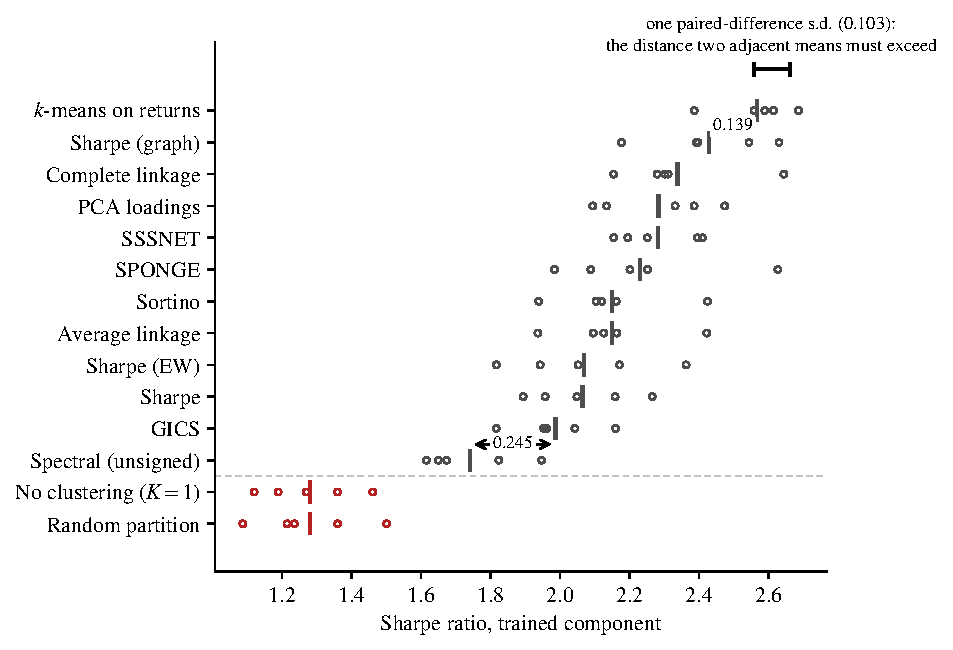
\includegraphics[width=\linewidth]{fig_field_ruler}
\caption{Per-seed Sharpe ratios against the dispersion of a gap. This figure plots
the per-seed Sharpe ratios of the 14 arms at the trained component over the
$6{,}913$-day window. Each row is one arm: circles are its five per-seed Sharpe ratios, the tick its mean. The bar at the top right is not an interval around a
center; its \emph{length} is one pooled paired-difference standard deviation, $0.103$, the distance two adjacent means must exceed, and it is meant to be laid
against the horizontal distance between two neighboring ticks. Nine of the 11
gaps between adjacent clusterizer means fall inside it; the two that do not are
marked, at the top and the bottom of the ranking. Measured on the levels instead the dispersion is $0.168$, and by that wider figure 10 of the 11 gaps fall inside. Both controls sit below every clusterizer run.}
\label{fig:field_ruler}
\end{figure}


\subsection{Variation across Partition Draws}
\label{sec:pseed}

The training-seed dispersion of \secref{sec:field} leaves out the variation in the partition itself. Every stochastic clusterizer's daily partitions were generated once and cached, and all five training runs use the same partitions (\secref{sec:seeds}). Redrawing the partition measures how much that draw moves the results. This subsection is reported on a different basis from the rest of the paper: five partition draws, each traded by a single training run at head seed $42$, so that the partition axis is isolated. The five training seeds of \secref{sec:seeds} do not enter here.

For the nine stochastic clusterizers, each redrawn five times (partition seeds $1$ to $5$; the cached partition of the rest of the paper is a separate draw), the adjusted Rand index (\textsc{ari}; \citealp{hubert1985comparing}) between two draws of the same clusterizer averages $0.30$, against $0.19$ between two different clusterizers. Expressed as disagreement, one minus the index, a redraw of the seed produces $87\%$ of the disagreement that a change of clusterizer produces. The average hides three levels that do not overlap. The four trading-driven clusterizers agree with their own redraw at $0.21$ to $0.28$, the four other stochastic clusterizers at $0.32$ to $0.45$, and \textsc{sssnet} at $0.18$, so stability against the seed is a property of the family.

Redrawing the partition moves the Sharpe ratios as well; the largest range grows from $0.21$ under the fixed rule to $0.38$ under the neural trading head, though not every clusterizer moves more. At the rule-based component, which has no training noise, the draw already moves the leader (\figref{fig:pseed_flip}a): spectral clustering is last under all five seeds, but $k$-means on returns is first under only three of them, Sharpe (graph) and PCA loadings under one each. The largest range across the five draws is $0.21$, for $k$-means on returns, $36\%$ of the $0.58$ between the best and the worst of the 45 rule-based books (nine clusterizers at five partition seeds); the random control, whose labels are redrawn daily under any seed, moves $0.08$.

Under the neural trading head the leader still depends on the draw and the movement is larger. When the head is rerun with its own seed pinned on the same redrawn partitions, $k$-means is first at four of the five draws and \textsc{sponge} at the other. The largest range across the five draws grows by three quarters, to $0.38$ for \textsc{sponge}, and the random control moves $0.39$
(\figref{fig:pseed_flip}b), as much as it moves across the five head seeds ($0.41$, \figref{fig:field_ruler}). The trained component, which might be expected to average the draw away, instead enlarges it, and for a partition that carries no information it converts the draw into as much variation as a refit does. \textsc{sssnet}, redrawn like the others, moves by $0.15$ at the rule-based component and by $0.13$ under the head, the fifth-largest and the smallest ranges among the nine. A ranking computed from one partition draw per clusterizer therefore carries a source of variation that rerunning the training leaves in place and enlarges.
%% ⚠ N84 (2026-09-01): sec:pseed now uses partition seeds {1,2,3,4,5} (head 42 pinned); the two comment blocks below describe the retired {42,1,123} basis. Numbers: repo analysis/results_5seed + figures/scripts/fig_pseed_flip_v3.py (computed from the books).
%% HEAD layer, 9 rules + random, head seed 42, ps{42,1,123}, ALL
%% verified vs run CSVs (2026-08-17 night, jobs 61623872+61637228):
%% kmeans 2.5443/2.6210/2.5784 (range .0767), pca_load
%% 2.3735/2.4243/2.3198 (.1045), spectral 2.2078/2.1632/2.1374
%% (.0704), sponge 2.4413/2.5239/2.2230 (.3009), sharpe_fixed
%% 2.4234/2.4076/2.2996 (.1238), sortino 2.4118/2.3573/2.2137
%% (.1981), fv2a 2.2199/2.2896/2.2259 (.0697), fv3sm
%% 2.5295/2.5803/2.3186 (.2617), random 1.2854/1.3431/1.5874 (.3020).
%% head/rule range ratios: fv2a .46, pca .46, kmeans .67 (damped);
%% spectral 1.39, sharpe_fixed 1.40, fv3sm 1.62, sponge 2.04,
%% sortino 3.94, random 6.81 (amplified).
%% WITHDRAWN on the full sample (do not restore): "the head damps the
%% partition draw" (was true only for the first four arms measured);
%% "random 0.30 is 4x any real rule" (sponge .3009 matches it);
%% "ordering identical under every seed" (true of the leader only).
%% Naive-layer numbers unchanged (paper basis, pseed_naive_paper_basis
%% + pseed_naive_RAW_OOS, cross-validated 4.9e-05).

\begin{figure}[tb]
\centering
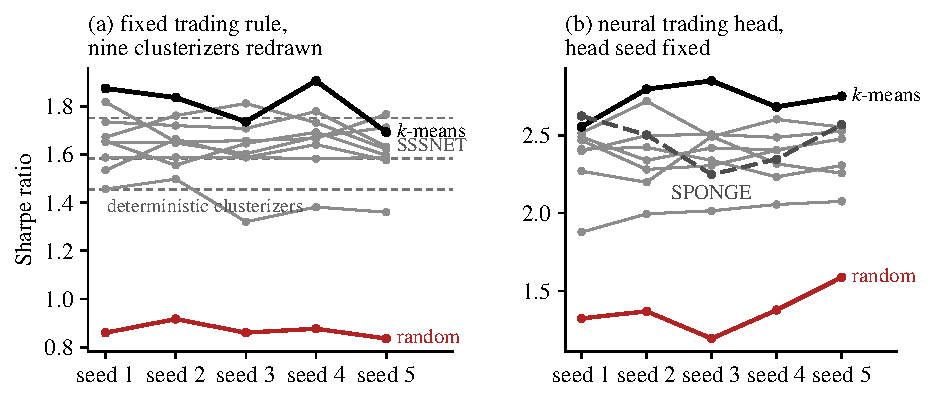
\includegraphics[width=\linewidth]{fig_pseed_flip}
\caption{Redrawing the partition seed at each trading component. This figure plots the Sharpe ratio of each stochastic clusterizer under five partition seeds. The labels on the horizontal axis name those partition seeds, not the training seeds of \secref{sec:seeds}, which are held fixed here. (a)
The rule-based component is deterministic, so every movement is the
partition draw itself. Spectral clustering is last under all five
seeds; $k$-means (black) is first under three of them, and the largest range is $0.21$. The panel tracks the nine stochastic clusterizers; the three deterministic ones, with no seed to redraw, are the dashed horizontals. (b) The trained component, with the head seed pinned at $42$ and the same nine clusterizers. $k$-means (black) is first at
seeds $2$ to $5$, \textsc{sponge} (dashed) at seed $1$. The largest range across the five draws is larger here than at the rule-based component, and so is the random control's. The random control is red in both
panels.}
\label{fig:pseed_flip}
\end{figure}

%%  ⚠ v3/cal6913 SENTINEL (N51-N53; supersedes the N22 block that stood
%%    here -- its naive-flip story and "up to 0.18" were V2 values):
%%    - naive layer: k-means FIRST under all three partition draws
%%      (1.7810/1.8735/1.9213); largest naive redraw range 0.23
%%      (Sharpe (EW), 0.2293); random moves 0.06 (0.0592).
%%    - trained layer (head seed pinned at 42): k-means first on two
%%      draws, sponge on the third; largest range 0.35 (Sharpe rule);
%%      random moves 0.09 (0.0894). Figure data = fig_pseed_flip_v3.py's
%%      NAIVE/HEAD dicts, independently reproduced to 4dp this campaign.
%%  ⚠ CAVEATS THAT MUST SURVIVE EDITING:
%%    - n = 3 partition draws;
%%    - the design is an L through the 3x3 grid: both marginals, no
%%      interaction. ⛔ no additive ANOVA over the two seed types.

\subsection{Formal Inference}
\label{sec:formal}



Formal tests reach the same conclusion, that the ranking separates its top from its bottom but not its neighbors. The comparisons above use no hypothesis test; \tabref{tab:formal} reports tests on the 12 clusterizers' seed-averaged books at the matched 60-day window, over the $6{,}913$ days all arms share. A model confidence set at the $90\%$ level keeps six of the 12 clusterizers, the six with the highest Sharpe ratios, so it divides the ranking in the middle rather than removing only the weakest arms; the two elimination statistics differ, $T_R$ keeping two. The set holds the partition draw of \secref{sec:pseed} fixed and could only widen with it. Pairwise Ledoit--Wolf tests find 21 of 66 differences that survive a Holm correction \citep{holm1979simple}, none of them between neighbors in the ranking. The adjacent pair closest to significance, the sector taxonomy against spectral clustering at the bottom of the ranking, has a raw bootstrap $p$-value of $0.004$ that the correction raises to $0.15$. The Sortino--Sharpe pair, the one clean objective contrast in the design, differs by $0.13$ with a standard error of $0.09$.

Part of the spread is the annualization itself. Daily Sharpe ratios are scaled by $\sqrt{252}$, which assumes away serial dependence. On non-overlapping $21$-day returns, $329$ blocks in place of $6{,}913$ days, the spread across the 12 seed-averaged books falls from $0.88$ to $0.40$, the $90\%$ set keeps 11 of the 12 under $T_{\max}$ and nine under $T_R$, and one of the 66 pairs survives Holm. The separation between clusterizers is visible day by day and modest at monthly frequency.

The gap to the controls survives at both horizons. Every clusterizer earns a higher Sharpe ratio than both controls, the confidence set discards both, and the pairwise gap is significant for all 12 against each control daily. At $21$ days five separate from $\K=1$ and five from the random control, a loss of power rather than a change of sign.

%%  THE CASE EITHER WAY, for the coauthors:
%%  CUT: §5.1-5.2 already make the point informally and more readably;
%%    this battery adds no new conclusion, its cells are on the OLD
%%    mixed-window set pending recompute, and the section is long.
%%  KEEP: it is the one place the paper speaks the venue's native
%%    inference language (MCS, Ledoit-Wolf, Holm, the annualization
%%    check) -- a JFEC referee may look specifically for it, and "we ran
%%    the formal battery and it agrees with the informal reading" is one
%%    short table. A middle path: keep the table, cut the prose to two
%%    sentences, or move the whole thing to the appendix with one
%%    pointer sentence here.
\begin{table}[tb]
\centering
\caption{Statistical tests on the 12 clusterizers}
\label{tab:formal}
\begin{threeparttable}
\footnotesize
\setlength{\tabcolsep}{4pt}
\begin{tabular}{@{}p{3.1cm}p{3.4cm}p{5.3cm}@{}}
\toprule
Procedure & Question & Result \\
\midrule
Model confidence set, $90\%$ & which clusterizers could be best?
  & keeps $6$ of $12$ under $T_{\max}$ and $2$ under $T_R$ \\
Ledoit--Wolf, all pairs & which differences are real?
  & $21$ of $66$ past Holm; none adjacent \\
Sortino vs.\ Sharpe & does the objective matter?
  & $+0.1260$ (s.e.\ $0.0919$) \\
Non-overlapping $21$-day returns & does $\sqrt{252}$ inflate the spread?
  & spread $0.8758 \to 0.4044$; $90\%$ set keeps $11$ of $12$ under $T_{\max}$, $9$ under $T_R$; $1$ of $66$ past Holm \\
Every clusterizer vs.\ both controls & do all clusterizers beat both controls?
  & yes: $12$ of $12$ above both, at both horizons \\
\bottomrule
\end{tabular}
\begin{tablenotes}[flushleft]\footnotesize
\item \emph{Notes.} This table reports the outcome of each test on the 12 clusterizers' seed-averaged payoffs; $T_{\max}$ and $T_R$ are the two elimination statistics of the model confidence set. All five rows are computed on one basis: the 12 clusterizers at the matched 60-day window, over the $6{,}913$ trading days every arm shares (\secref{sec:panel}), on seed-averaged payoffs, so the spreads are not comparable with the paired dispersion of \secref{sec:field}. Model confidence sets follow
\citet{hansen2011mcs}; pairwise tests follow \citet{ledoit2008robust}, on a circular block bootstrap (block $21$ trading days, $5{,}000$ draws, studentized bootstrap $p$-values). ``Past Holm'' counts the pairs whose difference survives the Holm step-down correction \citep{holm1979simple} over the $66$ pairs at the $5\%$ family-wise level.
\end{tablenotes}
\end{threeparttable}
\end{table}


\subsection{Between-Clusterizer Differences and the Choice among Clusterizers}
\label{sec:gradient}

Two different clusterizers' books correlate at $0.61$ on average in their daily position vectors. Whether $0.61$ is close or far requires a reference point, and the design supplies an internal one. Every
configuration is fitted five times (\secref{sec:seeds}), so we can
measure how much one clusterizer differs from itself when it is
refitted at a fixed partition. We run that comparison at three points along the pipeline
(\tabref{tab:gradient}): the partition, the positions it induces, and the payoff
those positions earn. At each point the comparison reports how much two different
clusterizers resemble each other, how much one clusterizer resembles itself under a
redraw of its own randomness, and the ratio of the two.

In the partition itself the ratio of the two indices is $0.65$ ($0.193$ against $0.296$), so two clusterizers resemble each other about two thirds as much as a clusterizer resembles its own redraw. Expressed as disagreement, one minus each index, the same two numbers give the result of \secref{sec:pseed}. In the positions the partition induces the ratio rises to $0.87$, and in the payoffs those positions earn it reaches $1.01$. Two different clusterizers produce payoffs that correlate as
strongly as one clusterizer does with itself refitted. 

\begin{table}[tb]
\centering
\caption{Similarity between clusterizers and to their own refits at three stages of the pipeline}
\label{tab:gradient}
\begin{threeparttable}
\small
\begin{tabular}{@{}lccc@{}}
\toprule
& Across clusterizers & Clusterizer against itself & Ratio \\
\midrule
Partition (\textsc{ari}) & $0.193$ & $0.296$ & $0.65$ \\
Positions, trained component    & $0.612$ & $0.704$ & $0.87$ \\
Daily payoff, trained component & $0.815$ & $0.805$ & $1.01$ \\
\bottomrule
\end{tabular}
\begin{tablenotes}[flushleft]\footnotesize
\item \emph{Notes.} This table reports how similar two clusterizers are at three stages of the pipeline, how similar a clusterizer is to its own refit, and the ratio of the two. \textsc{ari} is the adjusted Rand index. In the partition row the across-clusterizer cell covers all 66 pairs of the 12, while the against-itself cell covers the nine stochastic clusterizers, whose partitions were redrawn, on the refit days inside the same window; the position and payoff rows cover all 12 in both columns. The ``against itself'' column is likewise not the same object in every row: in the first row it is the same algorithm
at a redrawn \emph{partition} seed, in the last two the same partition
at a redrawn \emph{head} seed. Adjusted Rand indices are computed day
by day on the names two partitions share; every pair overlaps on at least $95\%$ of the names
except those involving the sector taxonomy, whose snapshot covers about
two thirds of the traded universe. Against either control the index is $0.000$ over all 24 pairs, which is why the controls are not shown. Positions are the daily weight vectors,
correlated across the union of the two books' names with absent names
entered at zero, on all $6{,}913$ common days and averaged over the five seeds. Payoff correlations are per seed and pair arms at the same
seed, so the seed is not itself a source of difference; seed-averaging the payoffs first raises the across-clusterizer figure to $0.886$ and is not comparable to the row shown. 
\end{tablenotes}
\end{threeparttable}
\end{table}

\figref{fig:bet_corr} shows that the resemblance is nearly uniform across pairs. No pair of clusterizers stands out and none falls away: the 12 clusterizers' pairwise position correlations run from $0.581$ to $0.657$, and every one of them lies between $81\%$ and $96\%$ of the diagonal of its own row. Sorting the clusterizers by Sharpe ratio produces no
block structure, so the arms at the bottom of the ranking hold much the same positions as the leaders, at higher volatility (\secref{sec:hedge}). The small differences that remain follow the families rather than the Sharpe ranking. The two hierarchical clusterizers are the most similar pair among the 12 ($0.657$ against an average of $0.61$ over all pairs) and the eigenstructure clusterizers are mildly cohesive ($0.635$). The four trading-driven
clusterizers, which share an objective but not a representation, are as similar to each other as to the other clusterizers ($0.604$ within, $0.604$ against the others).

\begin{figure}[tb]
\centering
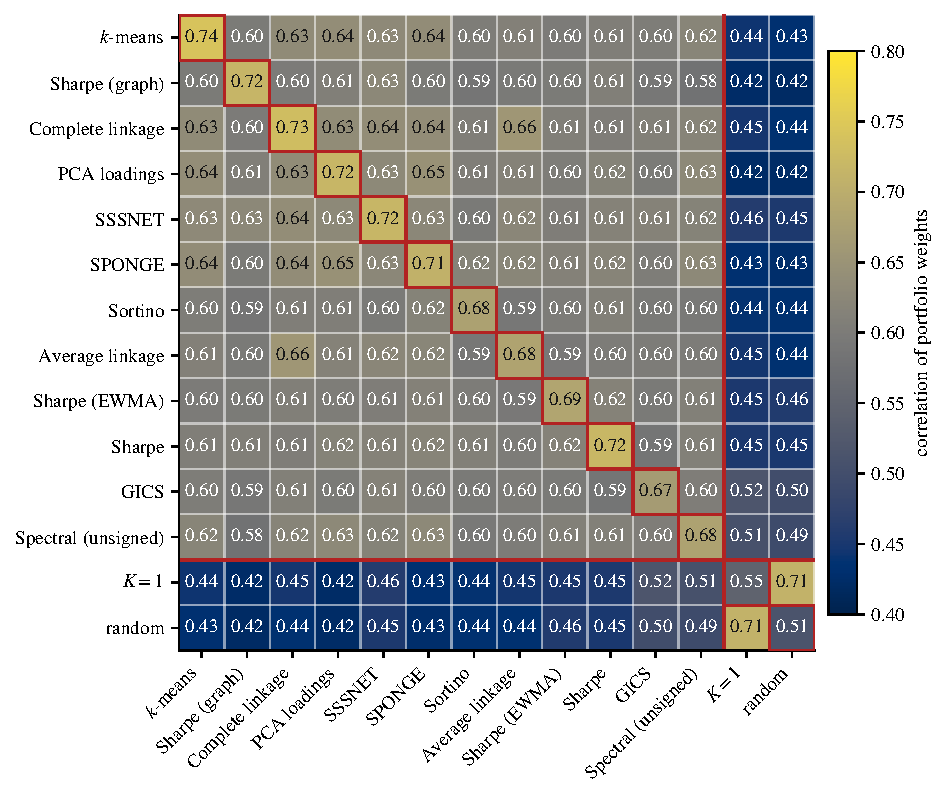
\includegraphics[width=\linewidth]{fig_bet_corr}
\caption{Position-vector correlation between arms. This figure shows the daily position-vector correlation between every pair of the 14 arms at the trained component over the common $6{,}913$-day window, ordered by Sharpe ratio. The diagonal is not one: it is each
arm against itself at a different seed, so every cell can be compared against the diagonal of its own row. The two controls are set off by a
divider line.}
\label{fig:bet_corr}
\end{figure}

The controls give a reference for how low the correlation falls between books that differ in substance. Relative to a clusterizer's correlation with its own refit, $0.704$, the correlation drops by $0.09$ between two clusterizers (to $0.612$) and by $0.25$ between a clusterizer and a control (to $0.450$); the first drop is $36\%$ of the second. The two controls correlate with each other at $0.71$, more than either correlates with its own refit under a redrawn head seed, $0.55$ and $0.51$; every clusterizer's own-refit correlation is $0.67$ to $0.74$. No clustering and a random partition therefore deliver much the same book, and retraining on a structureless signal is noisier than retraining on any partition. The instability is in the fit rather than the partition. The $\K=1$ control has no partition seed to redraw, and the random control's labels carry no structure under any seed, so the random control's Sharpe ratio moves as much when the label stream is redrawn as when the training seed is ($0.39$ across partition draws against $0.41$ across head seeds, \secref{sec:pseed}).

Because the 12 books are this similar, holding all of them at equal weight is as good as selecting among them. The equal-weight book earns a Sharpe ratio of $2.505$ on the seed-averaged payoff, above nine of the 12 books on that convention. Re-selecting the trailing best clusterizer each January leaves a gap to the equal-weight book whose confidence interval covers zero at every look-back considered (\figref{fig:select_vs_ew}). The match between equal weights and selection is the forecast-combination result in trading form: when candidates are exchangeable up to noise, equal weights are hard to beat \citep{timmermann2006forecast}.

Five of the 12 clusterizers, however, sit reliably below the equal-weight book, by $0.17$ to $0.60$ in Sharpe ratio; the intervals are from a circular block bootstrap over days (block $21$, $B = 5{,}000$). One of the five, Sharpe (EW), has a gap of $0.27$ against a range of $0.30$ across its own five partition draws, so its shortfall is not separated from the movement its own partition seed produces; of the other four, two clear their range and two have deterministic partitions and no such range to clear.
Three clusterizers score above the equal-weight book, $k$-means, Sharpe (graph), and complete linkage, by $0.27$, $0.13$, and $0.05$; only $k$-means' interval excludes zero, $[0.10, 0.44]$. Its margin of $0.27$ is about the size of the $0.29$ range its own five partition draws produce, so the one advantage the day bootstrap resolves is not separated from the partition axis. Differences of this size do not identify a best clusterizer. They do identify the clusterizers to avoid, and the clusterizers furthest below the equal-weight book are the most volatile (\secref{sec:hedge}).

\begin{figure}[tb]
\centering
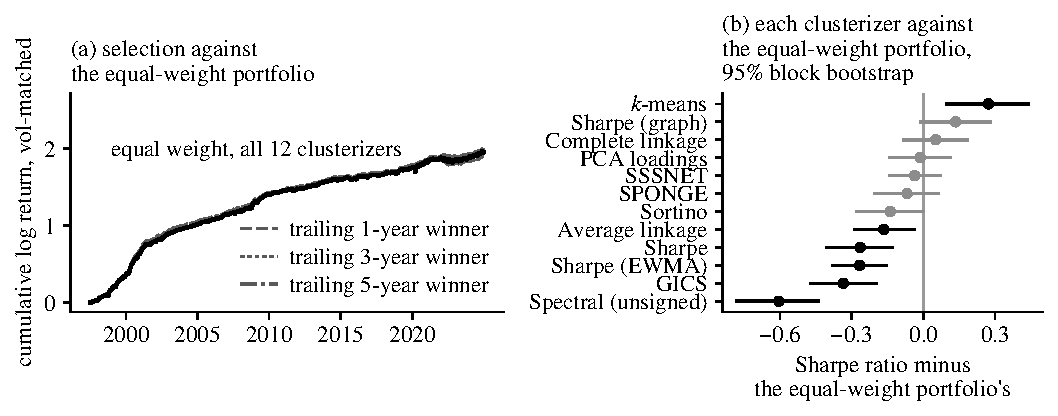
\includegraphics[width=\linewidth]{fig_select_vs_ew}
\caption{Selecting the trailing best clusterizer against holding all 12. This figure plots two comparisons of the seed-averaged trained books. (a) Cumulative log return of the equal-weight book and of three selection rules, each of which re-selects on the first trading day of each calendar year the clusterizer with the highest Sharpe ratio over the trailing one, three, or five years and holds it for the year; series are scaled to equal volatility. (b) Each clusterizer's Sharpe ratio minus the equal-weight book's, with $95\%$ circular block-bootstrap intervals (block $21$, $5{,}000$ draws). All books are seed-averaged trained books over the $6{,}913$-day sample, and panel (b) is ordered by that convention's Sharpe ratio rather than by the mean-of-per-seed ranking of \figref{fig:field_ruler}.}
\label{fig:select_vs_ew}
\end{figure}

%%  ⚠ 5.4 REWRITTEN 2026-08-20 on v3, then CORRECTED the same day after an
%%    adversarial pass. Every number recomputed from source on ALL 6,914
%%    common days (not a sample); script _reference/plot_bet_corr.py.
%%  ⛔ The rule-based POSITIONS row was withdrawn from tab:gradient. The
%%    author's hand-rolled naive book was never validated against the
%%    shipped naive Sharpes and is NOT the engine's book (the engine
%%    carries a 21-day correlation basis, a validity mask and a refit
%%    schedule; p1_lib.naive_stream). Restore the row only from a
%%    reimplementation that reproduces naive_routeA_v3_raw.csv, and
%%    persist the per-day books first -- there is currently no per-day
%%    payoff artifact for ANY v3 rule-based arm.
%%  ⛔ The ceiling footnote is mandatory (top-k exceeds 100%); do not let
%%    an edit turn the ceiling into a bound over all weightings.
%%  ⛔ Do NOT restore "every interval covers zero" as an unqualified claim
%%    about the twelve arms, and do NOT restore the "-0.08 to +0.08"
%%    selection range: that figure came from the v2 caption file and two
%%    independent v3 recomputes disagree with it and with each other.
%%    fig_select_vs_ew must be regenerated on v3 under one documented
%%    selection rule before it ships.
%%  ⚠ tab:onebet (0.87/0.83, PC1 88%/85%, 1.1/1.2 effective bets) was
%%    retired into tab:gradient's last row. v3 seed-averaged trained
%%    equivalents, if a referee wants them: rho-bar 0.866 on twelve,
%%    0.863 on the eleven of tab:gradient; PC1 87.7%.

\subsection{The Estimation Window and the Number of Groups}
\label{sec:window}
Two upstream inputs move the Sharpe ratio on the scale of the span between clusterizers: the length of a clusterizer's estimation window, which moves it by as much as the whole span, and the number of groups $\K$, which moves it by up to $0.36$ away from the $\K = 30$ used throughout, nearly half the span. The comparisons above hold both fixed. Holding the algorithm, the panel, the trading head, and the seeds fixed, we lengthen the window from $21$ days to $252$. Spectral clustering gains $+0.88$ in Sharpe ratio and PCA loadings $+0.66$, each monotone across the intermediate windows and paired by seed, while average linkage, which uses the same correlation matrix, moves $-0.00$. The difference between those responses is the clean comparison, because the arms use the same input; against average linkage, the window response of spectral clustering is $+0.88$ and of PCA loadings $+0.67$, the same sign in every seed. The two clusterizers that gain are the two that use individual eigenvectors of the correlation matrix, and three arms registered in advance to separate that account from its rival (that low starters gain most) move as the eigenvector account predicts (\appref{app:window}).

The number of groups is the second input. Of five clusterizers swept at $\K \in \{10, 30, 50\}$ (five seeds each, \appref{app:ksweep}), three rise monotonically in $\K$, while $k$-means on returns and spectral clustering peak at $30$ and fall by $0.09$ and $0.14$ between $30$ groups and $50$. For the four other than spectral clustering, coarsening to $10$ groups costs $0.20$ to $0.36$ in Sharpe ratio, and refining to $50$ changes it by $-0.09$ to $+0.22$. The gain from more groups cannot be split between finer structure and the finer demeaning of \secref{sec:mechanism} without a random control at each $\K$, which was not run; one run per $\K$ would not suffice (\appref{app:ksweep}). A downstream Sharpe ratio therefore distinguishes changes in the information supplied to the clusterizer and in the number of groups, but discriminates much less sharply among algorithms given the same input.

%% Source: discriminating cells, three seeds each, gate-clean,
%% spot-verified against recomputed SRs 2026-08-16 night:
%% agglo_avg@K10 w21 2.1011 -> w252 2.0873 (delta -0.0138, p=0.80);
%% pca_load@K50 2.0741 -> 2.9842 (+0.9101, p=0.002, CI [0.75,1.07]);
%% random@K30 1.4052 -> 1.3664 (-0.0388, p=0.67). Rival
%% delta = -0.8563*SR_w21 + 2.1866.
%%  ⚠ 5.5 GUARDRAILS (N20/N21):
%%  ⛔ never the t's (68.0, 30.96 -- degenerate denominators); effect
%%     sizes only, as drafted.
%%  ⛔ no "the window moves one rule further than the algorithm moves the
%%     field" -- withdrawn, reverses on 2 of 3 seeds paired.
%%  ⛔ kmeans_ret is NOT a window-unused control (window = its feature
%%     dimension, ARI(w21,w252)=0.143); its delta is "indistinguishable
%%     from zero, CI +/-0.41", not "no effect". Not drafted here at all,
%%     deliberately.
%%  ⛔ sponge +0.41 (p=0.045) left out of the prose: leave-one-seed-out
%%     fails 2 of 3, and its w120/w252 arms carry the GRAPH_LOOKBACK
%%     day-set confound (N22(e)). If an editor wants it, footnote it.
%%  ⚠ the discriminating experiment: first cell landed (agglo_avg@K10
%%     w21 2.1011, separation 0.377 vs sd 0.116) but the outcome cells
%%     had not; nothing printable yet.
%%
%%  ── EXHIBITS FOR THE REMAINING SUBSECTIONS%%
%%  ── EXHIBITS FOR THE REMAINING SUBSECTIONS ──────────────────────────
%%  5.3 formal tests: a TABLE, not a figure — test | question | result:
%%      MCS 90% (T_max) keeps 9/12 | T_R at rule-based keeps 3 | LW 7/66
%%      past Holm, none adjacent | Sortino-vs-Sharpe twin +0.0874
%%      (s.e. 0.0989) | non-overlapping 21-day sums: spread 0.5522 ->
%%      0.2155, 75% MCS keeps all twelve, 0/66.
%%      ⚠ ALL on the OLD mixed-window set — name it in the caption, and a
%%      matched-field recompute is on request to the compute branch.
%%  5.4 one bet in twelve costumes: REUSE fig_cum_pnl (already built —
%%      five arms' cumulative wealth, paths differing in roughness not
%%      drift) + the four numbers rho-bar 0.8325 / breadth 1.18 /
%%      PC1 84.7% / EW 99.17% of ceiling. ⚠ same old-set caveat.
%%  5.5 window: REUSE fig_window_twin (60 vs 21 with seed bands) — its
%%      caption already carries the right reading; add the DiD numbers
%%      (+0.578 / +0.784 vs agglo_avg) and the rival-model concession.

%%---------------------------------------------------------------------
%%  RESULTS 3 (§6).  07 opens it, 08 is its closing subsection §6.4.
%%---------------------------------------------------------------------
%!TEX root = ../main.tex
%%=====================================================================
%%  §7  NOT REDUNDANT GIVEN A FACTOR MODEL        drafted 2026-08-16
%%
%%  All numbers verified this session (workflow sec7-factor-verify +
%%  ff_lens run; records: _reference/CAPTIONS.md fig_lens_curve entries,
%%  NEWSTATS_hedge_w60.md calendar correction, ff_lens.csv).
%%
%%  SUPERSEDED — do not restore while editing:
%%   - 120-day lens values 0.2878 / 0.1644 / 57.1% / 25.83%  ->
%%     full-sample 0.2776 / 0.1712 / 61.7% / 23.22% (block SEs exist)
%%   - "19/19 unspanned, alpha 6.5-7.7, t 6.9-11.0, R2<=0.003" -> that
%%     was the same-day join on the old 19-arm set; this paper prints
%%     the matched 14 books on each layer's realization calendar
%%   - "no configuration retains less than 40%" -> dead; net of the
%%     matched floor it is 29-51% at m=5. Print the curve instead.
%%   - "the factor model explains almost none of these books" -> dead
%%     (join artifact); correct R2: rules <=0.10, k1 0.12, random 0.22
%%  STILL BINDING:
%%   - be fair to guijarro2025deep: their claim is in passing, under
%%     stated assumptions; we test it, we do not accuse them
%%   - do not conflate this section's "beyond classical factors" with
%%     the GICS-vs-methods comparison elsewhere; separate findings
%%   - GICS must be judged against ITS OWN floor 0.0344, never 0.0614
%%   - m_match is conditional; always pair it with the never-matched %
%%   - the six-named-factor removal ~= THREE PCs, less than five
%%     (0.190 vs 0.193 vs 0.171) — do not flip this comparison
%%   - AR/LM + Monte Carlo size study: prior campaign, different book;
%%     see the TODO below before citing them here
%%=====================================================================
\section{Factors, Peers, and Costs}
\label{sec:factor}

A partition is a special case of a factor model, and clustering-based trading is a special case of peer-based trading. As a factor model, a partition fixes each stock's loading at $1$ on its own group's mean and $0$ on every other group's mean. Latent factor models estimate the loadings freely \citep{fan2013large}. \citet{guijarro2025deep} remark in passing that ``under appropriate assumptions a clustering problem can be solved by a latent factor estimation.'' As a choice of peers, a partition gives every stock in a group the same peer set. The simplest alternative gives each stock its own peer set, the stocks most correlated with it. In this section, we ask whether baselines in either of these more general constructions already contain the information that a partition contributes. We test a partition against factor models in the cross-section and in the time series. In the cross-section, we measure how much of a partition's variance share remains after factors are projected out (\secref{sec:lens}). In the time series, we test whether the portfolios built on the partitions are spanned by the Fama--French five factors plus momentum, by a reversal factor, by the leading principal components, or by the portfolio of the same pipeline run without clustering (\secref{sec:spanning}). To test a partition against per-stock peers, we replace it with per-stock peer regressions and ask the same question of the portfolios (\secref{sec:peer}). Finally, we ask whether the portfolios remain profitable after trading costs (\secref{sec:costs}).

\subsection{Cross-Sectional Projections}
\label{sec:lens}

We ask how much of the cross-sectional variance of a day's market residuals a partition can explain, and how much of that it still explains after the leading principal components are projected out. If a low-dimensional latent factor representation captures the same cross-sectional structure as the partition, projecting out a few leading principal components should substantially reduce the variance share that the partition explains afterward. For each of the $6{,}913$ out-of-sample days, we take the day's cross-section of market residuals (\secref{sec:resid}) and apply the partition's same-day labels. We then record the variance share of \secref{sec:mechanism},
%
\begin{equation}\label{eq:vshare}
  \mathrm{VS}_t \;=\; 1 \;-\; \frac{\overbrace{\textstyle\sum_i s_{it}^2}^{\text{within-group variation}}}{\underbrace{\textstyle\sum_i \bigl(\tilde r_{it} - \bar{\tilde r}_t\bigr)^2}_{\text{total variation}}},
\end{equation}
%
where $\tilde r_{it}$ is the market residual of stock $i$ on day $t$, $s_{it}$ is its group-demeaned residual of \eqnref{eq:relsig}, and $\bar{\tilde r}_t$ is the cross-sectional mean of the market residuals. We use the stocks whose market residuals are complete over the loading window, the trailing $252$ days on which the principal components are estimated.\footnote{This leaves $322$ stocks a day for \textsc{gics} and $479$ to $500$ for the other 11 clusterizers. These stocks are not the same set as the $494$ stocks a day that the fixed trading rule trades in \secref{sec:mechanism}, so the variance shares reported there differ slightly from those here.} Next, we project out common factors. Let $B_t$ be the $\N_t \times m$ matrix of the stocks' loadings on $m$ factors. The projection replaces the vector of market residuals $\tilde r_t$ with
%
\begin{equation}\label{eq:proj}
  \tilde r_t^{\perp} \;=\; \tilde r_t \;-\; \underbrace{B_t \bigl(B_t^{\top} B_t\bigr)^{-1} B_t^{\top}\, \tilde r_t}_{\text{fitted by the factors}} .
\end{equation}
%
We write $\mathrm{VS}_t^{\perp}$ for \eqnref{eq:vshare} computed on $\tilde r_t^{\perp}$ with the same groups. For the principal components, $B_t$ holds the loadings on the leading $m$ principal components, estimated over the loading window and strictly before the day.

Projecting out the five leading principal components removes $39\%$ to $56\%$ of a real partition's variance share (\figref{fig:lens_curve}a). For example, with its singleton groups counted (\appref{app:lensrobust}), the $k$-means-on-residuals partition explains $26.5\%$ of the cross-sectional variance of the day's market residuals.
After five principal components are projected out, it still explains $16.0\%$ of the remainder. This is $60\%$ of its variance share before the projection. We call this ratio the retention,
%
\begin{equation}\label{eq:retention}
  \mathrm{Ret} \;=\; \frac{\sum_t \mathrm{VS}_t^{\perp}}{\sum_t \mathrm{VS}_t},
\end{equation}
%
where both sums run over the $6{,}913$ days. Across the 12
clusterizers, the retention at five principal components ranges from $44\%$ for
\textsc{gics} to $61\%$ for unsigned spectral clustering. By contrast, the random control's variance share is $6.00\%$ before the projection and $5.99\%$ after. Both values are at the degrees-of-freedom floor $(\K-1)/(\N-1) = 5.97\%$, the variance share that $\K$ random groups remove in expectation from any cross-section.\footnote{This floor is computed on the universe used here. On the traded universe of \secref{sec:mechanism}, the same formula gives the $5.88\%$ reported there.} The $\K=1$ control's variance share is zero by
construction.

We also count the leading principal components needed to match a partition's variance share, up to a maximum of $30$, the value of $\K$ (\figref{fig:match_cost}). For the $k$-means-on-residuals partition, $30$ principal components suffice on $79\%$ of days. On those days, about $17$ leading principal components are needed to match its variance share. On the other $21\%$ of days, even $30$ are not enough. For the other 11 partitions, the mean number of principal components needed is $7$ to $11$. For these partitions, $30$ principal components fall short on $0.2\%$ to $3.0\%$ of days. The block-bootstrap standard errors of the variance shares in this subsection are $0.1$ to $0.5$ percentage points, so we omit them from the figures.

The Fama--French factors absorb less than the five leading principal components. We repeat the measurement with the stocks' loadings on nested Fama--French sets (CAPM, then three, five, and six factors) as the columns of $B_t$ in \eqnref{eq:proj}. We estimate these loadings over the same loading window. After the full six-factor set is projected out, the 12 clusterizers keep
$50\%$ to $68\%$ of their variance shares before the projection
(\figref{fig:lens_curve}b). Every real partition's variance share declines gently and stays well above
the degrees-of-freedom floor. For example, the variance share of the $k$-means-on-residuals partition falls from $24.6\%$ after the CAPM projection to $20.6\%$ after three factors, $18.5\%$ after five factors, and $17.8\%$ after six factors. For $k$-means on residuals, the whole six-factor set removes about as much as three principal components and less than five. For all 12 clusterizers, the six factors remove less than five principal components. The random control keeps $99.9\%$ or more of its variance share under each of the seven projections. Its variance share equals the floor, which no projection can remove, so full retention is the expected result.

Loadings conditioned on characteristics absorb the least. We use the four
characteristics available on this panel: size, momentum, short-term
reversal, and realized volatility. Size is the log of market capitalization at the close of day $t$. Momentum is the return from day $t-252$ to day $t-21$, and short-term reversal is the return over the $21$ days ending on day $t$. Realized volatility is the standard deviation of raw returns over the $60$ days ending on day $t$. We standardize each characteristic across the day's cross-section and set a missing value to zero after standardization. When the columns of $B_t$ in \eqnref{eq:proj} are the four standardized characteristics, every real partition keeps
$77\%$ to $85\%$ of its variance share, more than it keeps after three principal
components are projected out. The principal components are estimated strictly before the day, but size, reversal, and volatility are measured through day $t$ itself and so contain that day's own return. Projecting out characteristics that contain the day's own return can remove more of the cross-sectional variance of the day's market residuals than projecting out characteristics measured before the day. The retention of $77\%$ to $85\%$ is therefore, if anything, too low. No factor model whose loadings are linear in these four characteristics can absorb more than this projection does, whatever its coefficients. The bound covers instrumented principal component analysis (IPCA) \citep{kelly2019characteristics}. On their own, the four characteristics explain $13\%$ of the cross-sectional variance of the day's market residuals. The random control's variance share again stays at its degrees-of-freedom floor. Accounting characteristics are not available on this panel, so the bound applies only to these four characteristics.

Under every projection, every real partition keeps a variance share above the degrees-of-freedom floor for its own numbers of groups and stocks. Net of that floor, the retention at five principal components ranges from $28\%$ to $49\%$ across the 12 clusterizers (\appref{app:lensrobust}).

\begin{figure}[tb]
\centering
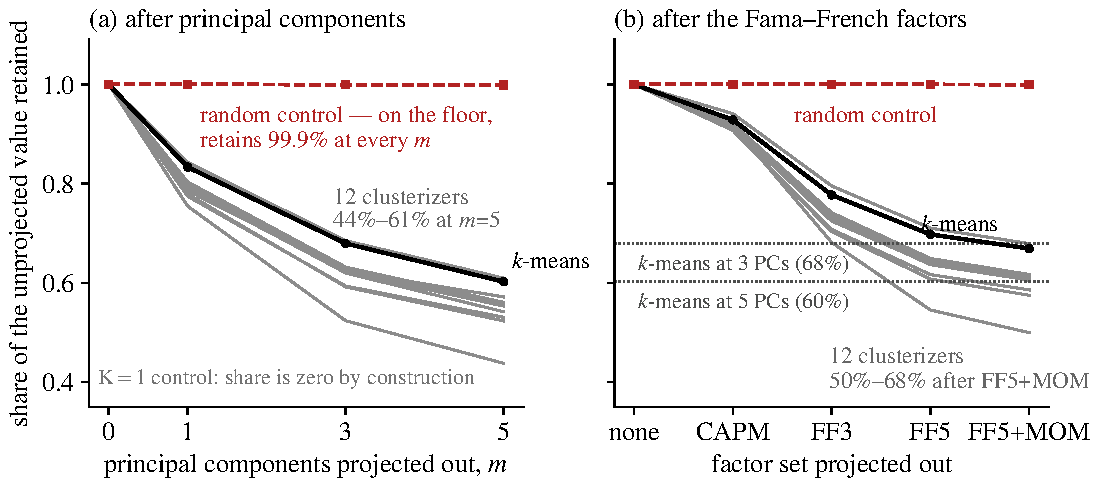
\includegraphics[width=\linewidth]{fig_lens_curve}
\caption{Variance share retained after projecting out principal components and after
projecting out Fama--French loadings. This figure plots each partition's retention (\eqnref{eq:retention}) over the $6{,}913$-day sample. The two panels share a
vertical axis, so the two projections can be compared directly.
(a) The leading principal components, with the first one, the first three, and the first five projected out. (b) The stocks' loadings on nested Fama--French sets, estimated
over the same $252$-day loading window as the principal components and on the aligned
calendar (\appref{app:calendar}). In panel (b), two dotted horizontal lines mark the retention of $k$-means on residuals in panel (a) at three and at five principal components. In both panels,
$k$-means on residuals is black and the other 11 clusterizers are gray. The dashed
red line is the random control, whose variance share is at the degrees-of-freedom floor $(\K-1)/(\N-1)$ and whose
retention is $99.9\%$ or more at every projection, because no projection can remove the floor. The $\K=1$
control's variance share is zero by construction.}
\label{fig:lens_curve}
\end{figure}

\begin{figure}[tb]
\centering
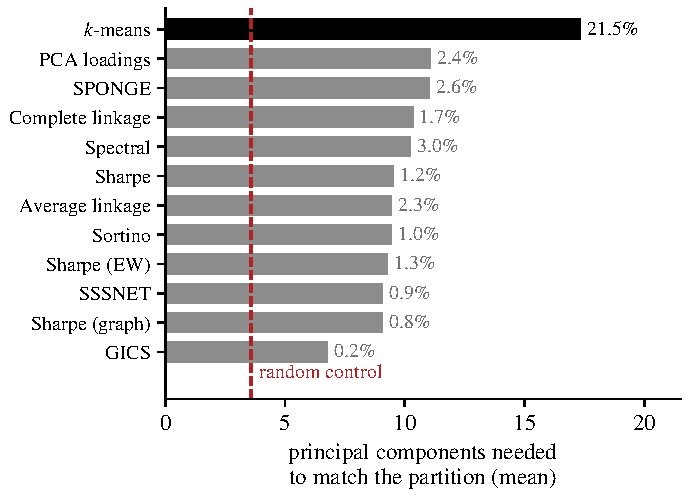
\includegraphics[width=.72\linewidth]{fig_match_cost}
\caption{Principal components needed to match a partition. This figure plots,
for each clusterizer, the mean number of leading principal components needed
to match its partition's variance share, over the
$6{,}913$-day sample. The search stops at $30$ principal components. The mean is taken
over the days on which $30$ suffice, and the percentage beside each bar is the
share of days on which they do not. The bar for $k$-means on residuals is black, and the bars for the other
11 clusterizers are gray. The dashed red line marks the random control.}
\label{fig:match_cost}
\end{figure}


\subsection{Portfolio Spanning Tests}
\label{sec:spanning}

In the time series, we test whether the standard factors span the portfolios' returns, that is, whether each portfolio's alpha against those factors is zero \citep{barillas2017alpha}. Under both trading models, we regress every portfolio's return on the Fama--French five factors \citep{fama2015five} plus momentum \citep{carhart1997persistence} (\tabref{tab:spanning}). For portfolio $p$, the regression is
%
\begin{equation}\label{eq:span}
  \pi_{pt} \;=\; \alpha_p \;+\; \underbrace{\beta_p^{\top} f_t}_{\text{factor exposure}} \;+\; u_{pt},
\end{equation}
%
where $\pi_{pt}$ is the portfolio return of \eqnref{eq:payoff} and $f_t$ is the vector of factor returns on the day on which the portfolio return is realized (\appref{app:calendar}). The later regressions in this section keep this form and change only the regressors in $f_t$. We find that no portfolio is spanned. Every alpha is positive, with $t$-statistics between $4.1$ and $10.7$. The factors explain little of the variation in any of these portfolio returns, with an $R^2$ of at most $0.21$ for the 12 clusterizers. The alphas of \secref{sec:hedge} are therefore not compensation for exposure to these factors.

These rejections are not artifacts of the finite-sample size of the $t$-tests. In a Monte Carlo calibrated to each portfolio's own tails and serial dependence, the empirical size of these tests is $6.6\%$ at a nominal $5\%$ level. Even for the worst-behaved portfolio, the corrected critical value is $2.2$ in $t$ units, which is well below the smallest $t$-statistic of $4.1$ (\appref{app:size}).

The fixed trading rule is a five-day reversal strategy, so the natural factor to add is a reversal factor. The short-term reversal factor of the French library is the closest traded factor, although it is formed on the return over the prior 20 trading days, against five days for the fixed trading rule. We add it to FF5+MOM in the lower block of \tabref{tab:spanning}. Under the fixed trading rule, the reversal factor explains $20\%$ to $25\%$ of the clusterizers' alphas and $38\%$ to $42\%$ of the controls' alphas (\figref{fig:reversal}). For example, the $\K=1$ control's alpha falls from $3.63\%$ to $2.11\%$. Every clusterizer's alpha remains at $3.09\%$ or more (\figref{fig:reversal} shows every value, and \tabref{tab:spanning} reports the ranges). The clusterizers' alpha advantage over the $\K=1$ control therefore widens from $+15.6\%$ to $+54.5\%$. Over the random control, it widens from $+13.1\%$ to $+42.8\%$. However, under the neural trading head, every portfolio loads on the reversal factor at $0.05$ to $0.07$, so the alphas fall by $8\%$ to $13\%$. The alpha advantage barely changes. All 28 portfolios remain unspanned.

The reversal factor is formed by sorting all stocks on their returns over the prior 20 trading days, so it captures reversal relative to the whole market. Demeaning within a real group removes this market-wide part of reversal from the signal and keeps the part that is relative to the group. As a result, under the fixed trading rule, the reversal factor explains more of the controls' alphas than of the clusterizers' alphas. This split of reversal into a market-wide part and a group-relative part follows the inter- and intra-industry decomposition of \citet{hameed2015industries} in spanning form. We use a statistical partition in place of industries and add the two controls, which the industry studies do not have. All portfolios of the neural trading head load lightly on the reversal factor, so they earn little of the reversal premium that the controls earn under the fixed trading rule. Because of this difference in exposure to the reversal factor, the alpha advantage under the fixed trading rule now exceeds that under the neural trading head. In \secref{sec:hedge}, the ordering was the reverse.

\begin{figure}[tb]
\centering
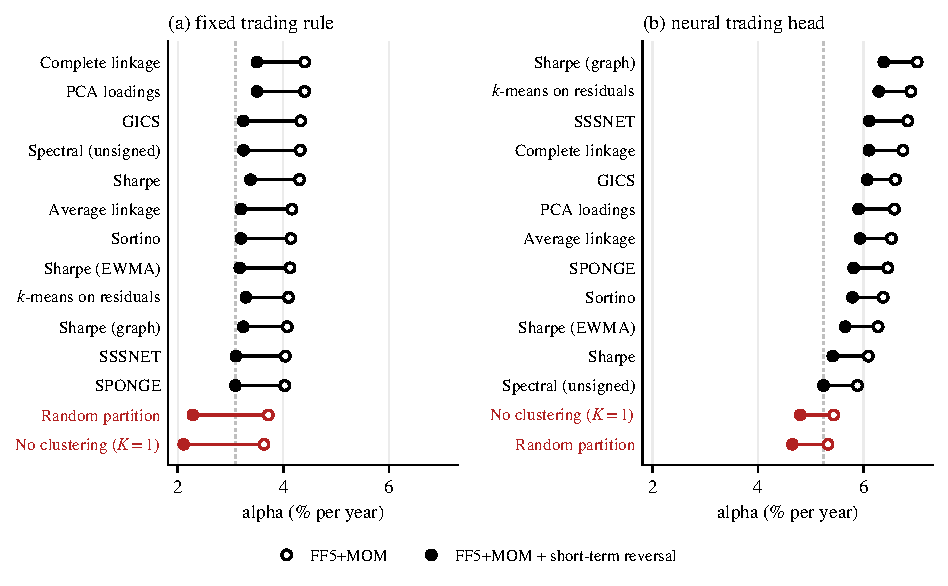
\includegraphics[width=\linewidth]{fig_reversal}
\caption{Alpha before and after the short-term reversal factor. This figure
plots, for each portfolio, its alpha on FF5+MOM (open circle) and its alpha once the
short-term reversal factor is added (filled circle), on the $6{,}913$-day
sample, from the regressions of \tabref{tab:spanning}. (a) The fixed trading rule; (b) the neural trading head. Within each panel, the portfolios are ordered by their FF5+MOM alpha. The two controls are red. The dotted vertical line marks
the lowest alpha with the reversal factor among the 12 clusterizers. Both trading models have gross exposure one, so the two panels share a horizontal axis.}
\label{fig:reversal}
\end{figure}

Although the five leading principal components absorb $39\%$ to $56\%$ of a partition's variance share (\secref{sec:lens}), they absorb almost none of the alpha of its portfolio. When we add the five leading principal components as daily factors, estimated over the same $252$-day loading window as in \secref{sec:lens}, every alpha in \tabref{tab:spanning} changes by at most $0.08$ percentage points, and every $R^2$ changes by at most $0.02$.\footnote{Each principal component's daily return is computed on the market residuals. It is the return of a portfolio with gross exposure one whose weights are the component's loading vector from the loading window. We align the sign of the loading vector from day to day. The five principal-component factors have annualized volatilities from $13.5\%$ down to $5.6\%$. Their premia are not statistically significant.}

The benchmark closest in construction to a clusterizer's portfolio is the portfolio of the same pipeline run without clustering. The $\K=1$ configuration of the same trading model shares the universe and the signal window with a clusterizer's configuration and differs from it only in the partition. To measure directly how much alpha a real partition adds, we therefore regress each clusterizer's portfolio and the random control's portfolio on the $\K=1$ portfolio (\tabref{tab:k1span}). Every clusterizer keeps alpha against the $\K=1$ portfolio. These alphas are $2.24\%$ to $2.86\%$ a year under the fixed trading rule and $2.39\%$ to $4.70\%$ under the neural trading head. Each of these alphas has a $t$-statistic of at least $5.8$. The clusterizers' portfolios load on the $\K=1$ portfolio at $0.37$ to $0.65$. Adding FF5+MOM to these regressions changes the alphas little. Against the $\K=1$ portfolio, each clusterizer keeps $52\%$ to $68\%$ of its FF5+MOM alpha (\tabref{tab:spanning}) under the fixed trading rule and $41\%$ to $68\%$ under the neural trading head. This remaining alpha comes from relative value within the group.

In contrast, the random control keeps little alpha. Under the fixed trading rule, its portfolio loads on the $\K=1$ portfolio at $0.93$, with an $R^2$ of $0.97$. Its alpha is $0.34\%$ ($t = 2.3$). Under the neural trading head, the random control's portfolio loads on the $\K=1$ portfolio at $0.90$, with an $R^2$ of $0.92$. Its alpha is $0.40\%$ ($t = 1.7$).




Under FF5+MOM, the factor loadings also distinguish the controls from the clusterizers. Under the neural trading head, the market loading is $0.105$ for the $\K=1$ control's portfolio and $0.093$ for the random control's portfolio. By comparison, the 12 clusterizers' portfolios load on the market at $0.051$ to $0.077$. Under the neural trading head, a real partition therefore leaves the portfolio with less factor exposure than no partition or a random partition does. This result is consistent with the lower volatility of the clusterizers' portfolios (\secref{sec:hedge}). Under the fixed trading rule, where each portfolio is dollar-neutral by construction, the factors explain little of any portfolio, with an $R^2$ of $0.05$ to $0.07$. The gap in market loading between the controls and the clusterizers is also smaller than under the neural trading head. The market loading is $0.023$ to $0.029$ for the clusterizers, $0.036$ for the $\K=1$ control, and $0.035$ for the random control.

The clusterizers' advantage over the controls holds after 2009 as well as before. When we split the sample at January 2009 (\tabref{tab:era}), alphas fall everywhere in the later subperiod, from $6\%$--$12\%$ to below $4\%$ a year. The clusterizers nevertheless remain separated from the controls in portfolio volatility, in the ordering of the alpha $t$-statistics, and, under the neural trading head, in the alpha advantage over the $\K=1$ control. First, in both subperiods and in both trading models, the controls' portfolios are more volatile than every clusterizer's portfolio. Second, although every alpha $t$-statistic falls, every clusterizer's $t$-statistic still exceeds those of both controls. Over $2009$--$2024$, the lowest clusterizer $t$-statistic under the neural trading head, $2.6$, narrowly exceeds the highest control $t$-statistic, $2.5$. Under the fixed trading rule over the same years, the lowest clusterizer $t$-statistic, $2.8$, exceeds the highest control $t$-statistic, $2.1$. Third, under the neural trading head, the alpha advantage over the $\K=1$ control is larger in the later subperiod, $+29.3\%$ over $2009$--$2024$ against $+20.2\%$ before. In the earlier subperiod, all 12 clusterizers earn more alpha than the $\K=1$ control. In the later subperiod, 11 of the 12 do so. The exception is unsigned spectral clustering.

After 2009, the ordering of the $t$-statistics also holds when we add the reversal factor. Specifically, under the fixed trading rule, the controls' alphas are then no longer significant ($t = 1.5$ for the $\K=1$ control and $1.7$ for the random control). By contrast, every clusterizer's alpha remains significant ($t$ from $2.6$ to $3.6$). Under the neural trading head, the controls keep their alphas in the post-2009 regressions with the reversal factor ($t = 2.1$ for the $\K=1$ control and $2.2$ for the random control). Every clusterizer's alpha has a higher $t$-statistic, from $2.3$ to $5.3$, although the lowest of them exceeds those of the controls by a small margin.

\begin{table}[tb]
\centering
\caption{Spanning against FF5+MOM, with and without a short-term reversal factor, within each trading model}
\label{tab:spanning}
\begin{threeparttable}
\footnotesize
\setlength{\tabcolsep}{2.5pt}
\begin{tabular}{@{}lcccccccc@{}}
\toprule
& \multicolumn{4}{c}{Fixed rule} &
  \multicolumn{4}{c}{Neural head} \\
\cmidrule(lr){2-5}\cmidrule(lr){6-9}
& $\alpha$ & $t_\alpha$ & $R^2$ & $\beta_{\mathrm{Rev}}$
& $\alpha$ & $t_\alpha$ & $R^2$ & $\beta_{\mathrm{Rev}}$ \\
\midrule
\multicolumn{9}{@{}l}{\emph{FF5+MOM}}\\
12 clusterizers & $4.03$--$4.40$ & $6.4$--$7.6$ & $0.05$--$0.07$ & --- & $5.89$--$7.02$ & $8.2$--$10.7$ & $0.14$--$0.21$ & --- \\
$\K=1$ & $3.63$ & $4.1$ & $0.05$ & --- & $5.44$ & $6.8$ & $0.24$ & --- \\
Random & $3.72$ & $4.4$ & $0.05$ & --- & $5.33$ & $7.1$ & $0.22$ & --- \\
\addlinespace
\multicolumn{9}{@{}l}{\emph{FF5+MOM+Reversal}}\\
12 clusterizers & $3.09$--$3.50$ & $5.3$--$6.6$ & $0.27$--$0.31$ & $0.08$--$0.11$ & $5.24$--$6.38$ & $7.5$--$10.4$ & $0.21$--$0.30$ & $0.05$--$0.07$ \\
$\K=1$ & $2.11$ & $2.5$ & $0.25$ & $0.15$ & $4.80$ & $6.1$ & $0.28$ & $0.06$ \\
Random & $2.29$ & $2.8$ & $0.25$ & $0.14$ & $4.65$ & $6.3$ & $0.27$ & $0.07$ \\
\bottomrule
\end{tabular}
\begin{tablenotes}[flushleft]\small
\item \emph{Notes.} This table reports spanning regressions of each portfolio's return on the six factors, and on the six factors plus a short-term reversal factor, under each trading model. The portfolios are those of the 12 clusterizers and the two controls at the common 60-day estimation window, on the $6{,}913$-day sample of \secref{sec:panel} (July 1997 to December 2024). Alphas are in percent a year. FF5+MOM is the Fama--French five factors plus momentum. Reversal is the daily short-term reversal factor (ST\_Rev) of the Ken French data library (CRSP vintage 202606): the average return of the two low-prior-return portfolios minus the average return of the two high-prior-return portfolios from $2 \times 3$ independent sorts on size and prior return, with prior return measured over days $-20$ to $-1$ and the portfolios formed daily. The loading on this factor is $\beta_{\mathrm{Rev}}$. Standard errors are Newey--West($21$) \citep{newey1987simple}. For the neural trading head, the regressions use the seed-averaged return. Each trading model is joined to the factor file on its own realization calendar (\appref{app:calendar}). Both trading models have gross exposure one (\secref{sec:components}).
\end{tablenotes}
\end{threeparttable}
\end{table}

\begin{table}[tb]
\centering
\caption{Spanning against the $\K=1$ portfolio of the same trading model}
\label{tab:k1span}
\begin{threeparttable}
\footnotesize
\setlength{\tabcolsep}{3.5pt}
\begin{tabular}{@{}lcccccc@{}}
\toprule
& \multicolumn{4}{c}{On the $\K=1$ portfolio} & \multicolumn{2}{c}{With FF5+MOM added} \\
\cmidrule(lr){2-5}\cmidrule(lr){6-7}
& $\alpha$ & $t_\alpha$ & $\beta$ & $R^2$ & $\alpha$ & $t_\alpha$ \\
\midrule
\multicolumn{7}{@{}l}{\emph{Fixed trading rule}}\\
12 clusterizers & $2.24$--$2.86$ & $6.9$--$8.2$ & $0.37$--$0.59$ & $0.53$--$0.81$ & $2.19$--$2.84$ & $6.9$--$8.3$ \\
Random & $0.34$ & $2.3$ & $0.93$ & $0.97$ & $0.32$ & $2.1$ \\
\addlinespace
\multicolumn{7}{@{}l}{\emph{Neural trading head}}\\
12 clusterizers & $2.39$--$4.70$ & $5.8$--$9.4$ & $0.42$--$0.65$ & $0.48$--$0.69$ & $2.46$--$4.77$ & $5.8$--$9.5$ \\
Random & $0.40$ & $1.7$ & $0.90$ & $0.92$ & $0.39$ & $1.7$ \\
\bottomrule
\end{tabular}
\begin{tablenotes}[flushleft]\small
\item \emph{Notes.} This table reports regressions of the return of each clusterizer's portfolio and of the random control's portfolio on the $\K=1$ portfolio of the same trading model. The $\K=1$ configuration shares the universe and the signal window with the other configurations of that trading model and differs from them only in the partition. The coefficient $\beta$ is the loading on the $\K=1$ portfolio. Alphas are in percent a year. The last two columns add FF5+MOM to the regressors. Sample, calendar, and conventions are those of \tabref{tab:spanning}, with Newey--West($21$) standard errors and, for the neural trading head, the seed-averaged return. The ranges cover the 12 clusterizers.
\end{tablenotes}
\end{threeparttable}
\end{table}

\begin{table}[tb]
\centering
\caption{Spanning against FF5+MOM by subperiod, 1997--2008 and 2009--2024}
\label{tab:era}
\begin{threeparttable}
\small
\begin{tabular}{@{}lcccccc@{}}
\toprule
& \multicolumn{3}{c}{$1997$--$2008$} & \multicolumn{3}{c}{$2009$--$2024$} \\
\cmidrule(lr){2-4}\cmidrule(lr){5-7}
& $\alpha$ (\%/yr) & $t_\alpha$ & $\sigma$ (\%/yr)
& $\alpha$ (\%/yr) & $t_\alpha$ & $\sigma$ (\%/yr) \\
\midrule
\multicolumn{7}{@{}l}{\emph{Neural trading head}}\\
12 clusterizers & $10.6$--$12.1$ & $9.1$--$10.4$ & $2.6$--$3.2$ & $2.0$--$3.2$ & $2.6$--$5.5$ & $2.7$--$3.6$ \\
$\K=1$ & $9.41$ & $7.0$ & $4.4$ & $2.15$ & $2.3$ & $4.4$ \\
Random & $9.29$ & $7.1$ & $4.2$ & $2.09$ & $2.5$ & $4.1$ \\
\addlinespace
\multicolumn{7}{@{}l}{\emph{Fixed trading rule}}\\
12 clusterizers & $7.1$--$8.1$ & $6.4$--$7.4$ & $2.6$--$3.3$ & $1.7$--$2.2$ & $2.8$--$3.9$ & $2.2$--$3.0$ \\
$\K=1$ & $6.45$ & $4.0$ & $5.2$ & $1.82$ & $1.9$ & $4.2$ \\
Random & $6.52$ & $4.3$ & $4.9$ & $1.89$ & $2.1$ & $4.0$ \\
\bottomrule
\end{tabular}
\begin{tablenotes}[flushleft]\small
\item \emph{Notes.} This table reports the spanning regressions of each portfolio's return on FF5+MOM, split at January $2009$, with the same series and calendars as the FF5+MOM block of \tabref{tab:spanning}, on the $6{,}913$-day sample of \secref{sec:panel}. Here, $\sigma$ is the subperiod's realized annualized volatility of the same series. For the neural trading head, $\sigma$ is therefore that of the seed-averaged return, the convention quoted in the notes to \tabref{tab:moments}. The volatilities in that table are instead computed per head seed and averaged over the five head seeds. 
\end{tablenotes}
\end{threeparttable}
\end{table}

\subsection{Per-Stock Peer Regressions}
\label{sec:peer}

We now turn to per-stock peer sets, from which we build two peer-regression portfolios on this panel. For every stock, we take as its peers the 20 stocks most correlated with it over the trailing $21$-day peer-selection window. We regress the stock's market residual, without an intercept, on the market residuals of its peers over a fit window of $60$ days for one portfolio and $252$ days for the other. The peer-regression residual of stock $i$ on day $t$ is
%
\begin{equation}\label{eq:peerres}
  \varepsilon_{it} \;=\; \tilde r_{it} \;-\; \underbrace{\sum_{j \in P_{it}} \hat b_{ij,t}\, \tilde r_{jt}}_{\text{peer fit}},
\end{equation}
%
where $P_{it}$ is the stock's peer set and $\hat b_{ij,t}$ are the fitted coefficients. The neural trading head takes $\varepsilon_{it}$ as input in place of the group-demeaned residual $s_{it}$. Different stocks' peer sets can overlap. However, no group of stocks shares a common peer set, so the construction does not involve a partition. Each peer-regression portfolio comes from a single run of the trading head at head seed $42$, so no standard deviation across head seeds is available for them. Peer selection is deterministic, so there is no partition seed to redraw either. We therefore do not compare their Sharpe ratios with those of the clusterizers.

In the cross-section, the peer construction absorbs much of a partition's variance share, considerably more than any of the factor projections above.
We repeat the measurement of \secref{sec:lens} after first removing the peer fit, the part of each stock's market residual fitted by its peers over a $60$-day fit window. For 10 of the 12 clusterizers, retention then falls to $25\%$ to $32\%$, against $44\%$ to $61\%$ across all clusterizers under five
principal components. The two exceptions are the $k$-means-on-residuals partition, which retains $52\%$, and \textsc{gics}, which retains $17\%$. The retention of $52\%$ for $k$-means on residuals is inflated by its singletons (\appref{app:lensrobust}). Projecting out the principal components \emph{after} the peer removal changes the retention by at most one percentage point for 10 of the 12 clusterizers and by at most five for the two exceptions. For this measurement, the principal components therefore add almost nothing to what the peer fit absorbs. The random control's variance share remains at its degrees-of-freedom floor through every stage, with a retention of $99.7\%$.

Although the peer fit absorbs much of a partition's variance share in the cross-section, some clusterizers' portfolios keep alpha against the peer-regression portfolios in the time series. We regress the return of every portfolio of the neural trading head on the two peer-regression portfolios,
on FF5+MOM, and on both together (\tabref{tab:peer}). Against FF5+MOM alone, every portfolio keeps its alpha, as in \secref{sec:spanning}. However, against the peer-regression portfolios, the controls and the clusterizers differ. Both controls lose their alpha entirely, with an alpha of $-1.6\%$ a year ($t=-2.2$) for the $\K=1$ portfolio and $-1.4\%$ ($t=-2.0$) for the random control's portfolio. The two peer-regression portfolios therefore explain all of the alpha that this pipeline
earns without a real partition. In contrast, four of the 12 clusterizers keep their alpha, $0.8\%$ to $1.5\%$ a year, with $t$ between $2.1$ and $3.9$. The alphas of the other eight range from $-0.81\%$ to $0.74\%$ ($t$ from $-1.7$ to $1.8$). Unsigned spectral clustering has the lowest of these alphas. Its Sharpe ratio is no higher at $50$ groups than at $10$ (\secref{sec:window}). Among the 12 clusterizers, its portfolio also has the highest volatility (\secref{sec:hedge}) and is furthest below the equal-weight portfolio in Sharpe ratio (\secref{sec:gradient}).

In \eqnref{eq:span}, adding the six factors to the two peer-regression portfolios in $f_t$ raises the alpha of all 12 clusterizers' portfolios by $0.17$ to $0.47$ percentage points. Because the regression has an intercept, the estimated alpha is
%
\begin{equation}\label{eq:alphaid}
  \hat\alpha_p \;=\; \underbrace{\bar\pi_p}_{\text{mean return}} \;-\; \underbrace{\hat\beta_p^{\top} \bar f}_{\text{loadings} \,\times\, \text{mean factor returns}} .
\end{equation}
%
When the factors enter the regression, every clusterizer's portfolio loads less on both peer-regression portfolios. Because the peer-regression portfolios earn positive mean returns, these lower loadings raise $\hat\alpha_p$ in \eqnref{eq:alphaid}. The small positive market loadings of the clusterizers' portfolios offset part of this increase. Adding the reversal factor as well changes the alphas by at most $0.11$ percentage points, because the peer-regression portfolios already absorb the part of the returns that the reversal factor would absorb. The factors raise the alphas and remove common variation from the regression residual. Both effects increase the $t$-statistics. Against the peer-regression portfolios and the factors together, eight of the 12 clusterizers have a $t$-statistic above $1.96$, against four on the peer-regression portfolios alone.

The two controls show that the alpha that the clusterizers keep against the peer-regression portfolios comes from the partition. The controls share the market residuals, the signal window, and the trading head with the clusterizers. They differ from the clusterizers only in the partition, which is absent in the $\K=1$ control and random in the random control. If the shared stages produced the alpha, the controls would also keep a positive alpha against the peer-regression portfolios. Instead, the alphas of both controls are negative, with or without the factors (\tabref{tab:peer}).

Conversely, when we regress each peer-regression portfolio on the equal-weight portfolio of all 12 clusterizers, the alpha is $2.5\%$ a year ($t = 5.5$) for the $60$-day fit and $2.3\%$ ($t = 6.8$) for the $252$-day fit. Although partitions and per-stock peer regressions capture much the same comovement, neither explains all of the other's alpha in our setting. The $R^2$ of a clusterizer's portfolio return on the peer-regression portfolios is positively related to its Sharpe ratio. However, the relation falls just short of significance at the $5\%$ level (\appref{app:peerdist}).

\begin{table}[tb]
\centering
\caption{Spanning against peer-regression portfolios, factors, and both}
\label{tab:peer}
\begin{threeparttable}
\small
\setlength{\tabcolsep}{3pt}
\begin{tabular}{@{}>{\raggedright\arraybackslash}p{3.9cm}cccccc@{}}
\toprule
& \multicolumn{2}{c}{On the peer-regression portfolios}
& \multicolumn{2}{c}{On the six factors}
& \multicolumn{2}{c}{On both} \\
\cmidrule(lr){2-3}\cmidrule(lr){4-5}\cmidrule(lr){6-7}
& $\alpha$ (\%/yr) & $t_\alpha$ & $\alpha$ (\%/yr) & $t_\alpha$ & $\alpha$ (\%/yr) & $t_\alpha$ \\
\midrule
12 clusterizers\tnote{a} & $-0.81$--$1.45$ & $-1.7$--$3.9$ & $5.89$--$7.02$ & $8.2$--$10.7$ & $-0.35$--$1.68$ & $-0.7$--$4.5$ \\
$\K=1$ & $-1.63$ & $-2.2$ & $5.44$ & $6.8$ & $-0.82$ & $-1.2$ \\
Random & $-1.42$ & $-2.0$ & $5.33$ & $7.1$ & $-0.74$ & $-1.1$ \\
\addlinespace
Peer-regression portfolio, $60$-day fit, on the clusterizers' equal-weight portfolio & $2.52$ & $5.5$ & & & & \\
Peer-regression portfolio, $252$-day fit, on the clusterizers' equal-weight portfolio & $2.32$ & $6.8$ & & & & \\
\bottomrule
\end{tabular}
\begin{tablenotes}[flushleft]\footnotesize
\item \emph{Notes.} This table reports, for the neural trading head, spanning regressions of each portfolio's return on the two peer-regression portfolios, on the six factors (the Fama--French five factors plus momentum), and on both. The table also reports the regression of each peer-regression portfolio on the equal-weight portfolio of the 12 clusterizers. In the last two rows, the first pair of columns reports the alpha and $t$-statistic of each peer-regression portfolio on that equal-weight portfolio. Alphas are in percent a year. The six-factor columns repeat the regressions of the neural trading head in the FF5+MOM block of \tabref{tab:spanning} for comparison. The clusterizers' portfolio returns are seed-averaged over the five head seeds, and the peer-regression portfolios come from single runs at head seed $42$. All series are panel-internal, so the regressions share
a common calendar. The factor file is joined at a one-day lag, as for every return series of the neural trading head (\appref{app:calendar}). The $t$-statistics are computed with Newey--West($21$) standard errors.
\item[a] All three ranges cover the 12 clusterizers. On the peer-regression portfolios, four of the 12 keep a $t$-statistic above $1.96$. On the peer-regression portfolios and the six factors together, eight do.
\end{tablenotes}
\end{threeparttable}
\end{table}

%%  §7.3 REWRITTEN 2026-08-21 on v3. Every number recomputed from source
%%  this session: the three spanning specifications from the run logs
%%  with factor_lens.spanning.nw_ols, the retention column from the v3
%%  peer lens (job 61975607, all 6,914 days), the position overlaps from
%%  the verified weight files.
%%  ⛔ HELD BACK, do not add without the runs: (i) any LEVEL comparison
%%     between the peer class and the clusterizers -- the peer arms have
%%     one seed each, so 2.98 against the field's best 2.94 sits inside a
%%     ruler of 0.094 with no dispersion on one side; (ii) the finding
%%     that the peer fit window diversifies where a clusterizer's does
%%     not (peer w60/w252 correlate 0.52 against 0.87-0.89 for pca_load,
%%     agglo_avg and spectral) -- two windows is not a sweep. Both are
%%     requested from the compute branch (seeds on w60/w252, plus w21 and
%%     w120).
%%  ⚠ The peer lens ran with an EMPTY anchor: the v2 npz check was
%%     removed for v3 and the reported "anchor max diff 0.00" is vacuous.
%%     The retention denominators were cross-checked independently here
%%     (unconditional R2 by arm, 300-day sample, agrees within 1 point
%%     and reproduces the ordering); the numerators have no second source.

%%=====================================================================
%%  §6.4  merged from 07_costs.tex on 2026-08-27 (user request)
%%=====================================================================
%%=====================================================================
%%  §8  NOTHING SURVIVES FIVE BASIS POINTS      target 2 pp. NO MORE.
%%
%%  THIS SECTION IS SCOPE, NEVER ARGUMENT. The venue audit calls the
%%  generated draft's six-subsection version "the longest single venue
%%  liability". Two pages, one table, one figure.
%%
%%  ⚠ MANDATORY CAPTION LINE, 2026-08-15 (CORRECTIONS.md N22(h)).
%%    THE COST ROWS ARE NOT AT THE SAME WINDOW AS THE HEADLINE TABLE.
%%    netcost/sbatch_netcost.sh:45-50 routes five arms to their w21
%%    partitions: fv2a, fv3sm, sharpe_fixed and sortino explicitly (their
%%    work.py all read CORR_LOOKBACK = 21), and SPONGE through the
%%    wildcard *) branch to labelcache_sponge_K30_daily_full.pkl, whose
%%    32,423,016-byte signature is the w21 file and not its 32,088,563
%%    w60 twin. SPONGE is the one no reader would suspect, because
%%    nothing in its name or its branch says w21.
%%    ⛔ No netcost/runs/* directory has a MANIFEST, so byte size is the
%%       only in-band proof. Any future netcost pass must write one.
%%
%%    PRINT THIS, FLATLY, AND CLAIM NOTHING BEYOND IT:
%%      "Cost rows are computed at each arm's native clustering window;
%%       for [the five] that is 21 days rather than the 60 used in
%%       Table N."
%%    ⛔ DO NOT add "the difference is unlikely to matter". I asserted
%%       that and it does not survive our own record: N20(e) measures the
%%       traded book as window-INVARIANT for pca_load, agglo_complete and
%%       spectral_unsigned but NOT for agglo_avg (0.158%) or kmeans_ret
%%       (0.615%), driven by singleton frequency, which is itself
%%       window-dependent. Turnover is a function of book size and
%%       membership churn, so window-insensitive turnover is an
%%       assumption the same section contradicts for some arms. Checking
%%       it needs w60 cost runs for those five, which do not exist.
%%
%%  CONTENT:
%%   * 0 of 16 configurations net positive at 5 bps
%%   * turnover 36.5-54.3 %/day, break-even 2.23-3.60 bps
%%   * the structural reason, which connects back to §5: gross return is
%%     6.5-7.7 %/yr against roughly 11.8 %/yr of cost at that level. The
%%     first moment is fixed and modest; turnover exceeds it. This is not
%%     a defect of one implementation
%%   * costs REORDER the field -- the lowest-turnover clustering rises
%%     sharply once costs are charged -- which shows the gross ordering
%%     is not an ordering of economic value
%%   * ⚠ charging five basis points is NOT a monotone transformation of
%%     the gross ranking. Say so; it is the interesting part
%%
%%  COMPARISON TO THE NEAREST PAPER, stated carefully:
%%   brutti2026orthogonal report that clustering REDUCES turnover sharply
%%   in their setup (87.9% to 24.2-24.4%) and do not charge costs at all,
%%   while our configurations show no such gap. Flag the divergence, name
%%   rebalancing frequency as the likely cause, and label it AN OPEN
%%   QUESTION WE HAVE NOT MEASURED. Do not present it as a finding.
%%
%%  LIMITATIONS PARAGRAPH: no market-impact model, no borrow costs, US
%%  large caps only, one residualization scheme, and -- state it here --
%%  K fixed at 30 throughout, with the sweep that would settle whether
%%  the input-parameter result generalizes still unrun.
%%
%%  ⛔ ANY tradability or deployability claim, anywhere in the paper.
%%=====================================================================
\subsection{Transaction Costs}
\label{sec:costs}
The last question is whether the portfolios remain profitable after trading costs.
We measure the daily one-way turnover of a portfolio as $\tfrac{1}{2}\sum_i |w_{it} - w_{i,t-1}|$. Because the gross exposure is one, this turnover is the fraction of the portfolio traded each day. For the 14 portfolios of the neural trading head, it averages $38.2\%$ to $46.9\%$. Turnover varies much less across the 14 portfolios than the gross Sharpe ratio does. The highest turnover is $23\%$ above the lowest, whereas the highest gross Sharpe ratio is $101\%$ above the lowest. The break-even cost is $2.7$ to $3.8$ basis points one-way. At daily rebalancing, every portfolio has a negative net return at five basis points.

At costs below break-even, the net Sharpe ranking follows the gross ranking. At five basis points, it follows turnover. Turnover is not a measure of clustering quality. At one and two basis points, the two controls
remain the two lowest of the 14 portfolios, below each of the 12 clusterizers
in net Sharpe ratio. The rank correlation between the net and the gross ordering is $\rho = 0.98$ at one basis point and $0.91$ at two.

At five basis points, the net ranking largely stops following the gross ranking. The rank correlation with the gross ranking falls to about $0.3$. For example, \textsc{gics} ranks eleventh of the 12 on gross Sharpe ratio but is the least negative portfolio at five basis points. The portfolio of $k$-means on residuals falls from first to seventh of the 14 portfolios. To three decimals, its net Sharpe ratio equals that of unsigned spectral clustering. Both controls move up among the clusterizers. The $\K=1$ control ranks above four of the 12 clusterizers. The random control ranks above one. The \textsc{gics} portfolio rises furthest. This could suggest that a taxonomy has low trading costs, because its labels rarely change. However, the \textsc{gics} portfolio is also the one that depends least on its own labels. On a given day, about $35\%$ of the stocks it trades are not covered by the sector table and are assigned to the group they correlate with most strongly (\tabref{tab:methods}, note e). As a result, the
low turnover of \textsc{gics} cannot be attributed to the taxonomy alone. Average linkage, which does not use a taxonomy, shows the same reordering. Its portfolio turns over $39.7\%$ a day and finishes fourth at five basis points. The gross ranking therefore does not order the portfolios by their value after trading costs. Every comparison in \secsref{sec:riskreturn}{sec:invariance} compares gross performance, before trading costs. Under the fixed trading rule, every clusterizer's portfolio earns a higher gross Sharpe ratio than the portfolio of the $\K=1$ control, $1.46$ to $1.78$ against $0.83$. \citet{brutti2026orthogonal} also find that every clustering-based portfolio earns a higher Sharpe ratio than their no-clustering benchmark. However, our portfolios do not show the turnover reduction that they report. In \appref{app:costs}, we give the cost model, the full table, the same measurement on the fixed trading rule, the comparison with that study, and the limitations of the exercise.

%!TEX root = ../main.tex
%%=====================================================================
%%  §9  CONCLUSION                            target 1-1.5 pp.
%%
%%  REWRITTEN 2026-08-16 to match the final abstract/intro (user's
%%  abstract structure: two goods -> family comparison -> head ->
%%  factor -> costs). No new numbers; every sentence restates a
%%  section, none more strongly than the section did.
%%
%%  ⛔ Do not introduce a result here. Bans that bite in this file:
%%   - no post-2009 alpha edge over K=1 (era scope: pre-2009 only)
%%   - "cannot rank" must stay at §5's strength ("not a resolvable
%%     object"; the top and bottom gaps DO resolve)
%%   - no tradability claim; no "largely absorbs" (only partly, and
%%     only vs K=1)
%%=====================================================================
\section{Conclusion}
\label{sec:conclusion}

This paper separates the two decisions a clustering-based statistical arbitrage strategy makes: how to group stocks and what model to trade within the groups. It measures what the clustering contributes against a no-clustering control and a random-partition control, at a fixed trading rule and under a neural trading head. A real partition lowers the volatility of the book, by about $40\%$ relative to either control under the fixed rule, and raises its alpha. The volatility reduction belongs to the clustering and every clusterizer supplies it; the neural trading head widens the alpha advantage, most against the random partition, so a wrong partition costs more under a fitted model.

More broadly, informative clustering is much easier to distinguish from the controls than competing clustering algorithms are from one another. Whether an informative partition is used matters far more than which one. The 12 clusterizers disagree about the partition but largely agree about the book, and their Sharpe ratios differ mainly through the volatility of their books. Their payoffs correlate with one another as strongly as with their own refits, most adjacent clusterizers in the Sharpe ranking are closer together than the run-to-run variation in their gap, and redrawing the partition seed changes the leader at both trading components. A downstream Sharpe ratio distinguishes changes in the information a clusterizer uses and in the number of groups it forms; given the same input, it discriminates much less sharply among algorithms. Ex ante selection on past performance does not outperform a simple equal-weight combination of the 12 books.

The comovement a partition captures is only partly absorbed by principal components or by the Fama--French factors in the cross-section, and the partition's books are not spanned by either, by a short-term reversal factor, or by the same strategy traded without clustering. Per-stock peer regressions absorb much of what a partition explains in the cross-section, yet most of the 12 clusterizer books keep their alpha against the peer books and the factors together, and the peer books keep theirs against the equal weight of all 12. The two constructions appear to differ in the class of peer set, shared or per-stock, rather than in the choice within a class. None of these books survives a five-basis-point one-way cost at daily rebalancing: break-even sits below four basis points one-way, and at five no book is net positive.

Two rules for evaluating partitions follow. A comparison of partitions should include a trading component with no fitted parameter, so that what the partition contributes is not confounded with what the model fits; a fitted model narrows the volatility benefit and widens the alpha benefit. A ranking of partitions should first check its gaps against seed and partition-draw noise. The two controls, the two noise benchmarks, and the split of the Sharpe gap into its mean and volatility parts apply unchanged to the comparison between shared and per-stock peer sets, which is the open question this design leaves.



\section*{Conflicts of interest}
The authors declare that they have no competing interests.

\section*{Funding}
Yixuan He is supported by an NVIDIA Academic Grant Award as well as a Jetstream2 AI Fellowship.

%% Data availability statement goes here once the replication
%% repository is organized (user decision 2026-08-24: deferred).

\section*{Acknowledgments}
The computations in this article were performed on an NVIDIA GPU
server awarded to Yixuan He and on the Sol supercomputer at Arizona
State University; we thank NVIDIA Corporation and ASU Research
Computing for these resources.

\bibliographystyle{oup-abbrvnat}
\bibliography{refs}

\begin{appendices}
%!TEX root = ../main.tex
%%=====================================================================
%%  APPENDIX
%%
%%  WHAT STAYS HERE, now that §4 exists:
%%   A.1  full per-configuration results, both trading layers, with seed
%%        standard deviations and era breakdowns
%%   A.2  the twelve methods in detail (moved out of §3)
%%   A.3  the aggregation identity with its derivation and reconstruction
%%        error
%%   A.4  the Monte Carlo size table for the spanning statistics
%%   A.5  the stacked-factor experiment, if included at all
%%   A.6  implementation and replication: the validity screen, the seed
%%        protocol, the note that the hardware is non-deterministic so
%%        exact reproduction is bounded at |dSR| <= 0.08, and THE TWO
%%        SHARPE CONVENTIONS with a conversion note
%%
%%  WHAT MOVED OUT, to §4: the two standard errors and their derivation,
%%  the rho^2 correction, the reliability calculation, the calibrated
%%  simulation. Those are the paper's econometrics and they belong in the
%%  body.
%%
%%  FRONT MATTER THE AUTHORS MUST SUPPLY:
%%   * Yixuan He's affiliation -- nothing in the repository states it
%%   * Lunji Zhu's email
%%   * any grant or data acknowledgement, or none
%%=====================================================================
\section{Appendix: Data, Implementation, and Additional Results}
\label{app:supp}

This appendix has two parts. \appref{app:rules} to \appref{app:calendar} give the construction of each clusterizer, the treatment of degenerate groups, the realized partition sizes, the trading head's architecture and schedule, the identifiers under which every arm was run, the sweep over the number of groups, and the calendar offset between the panel and the factor file. \appref{app:dose} to \appref{app:costs} give the additional results the text refers to, in the order in which the text refers to them: an experiment that degrades a real partition continuously toward a random one, the mechanism behind the estimation-window effect, three robustness checks on the factor and peer comparisons, and the transaction-cost calculation in full. Data and code are submitted with the replication files.

\subsection{The Clusterizers in Detail}
\label{app:rules}

All clusterizers receive the same input: the day's universe of $\N_t$ stocks
(\secref{sec:panel}) and the trailing window of market residuals
$\mathbf{R}_{\mathrm{tr}} \in \real^{60 \times \N_t}$, 60 days ending
at $t$. All target $\K = 30$ groups. Where a correlation matrix appears
it is $\Cmat = \operatorname{corr}(\mathbf{R}_{\mathrm{tr}})$, the
$\N_t \times \N_t$ sample correlation of the window's columns.

\paragraph{$k$-means on returns.} Each stock is treated as the point of
its own 60 residual returns in $\real^{60}$, and $k$-means with
Euclidean distance partitions those points ($30$ clusters, $4$
restarts). No correlation matrix is formed. Because the coordinates are
unstandardized, distance is dominated by volatility. High-volatility names sit far from everything and often become singletons (about 10 a
day), whose members the trading stage later drops (\tabref{tab:methods}, note b).

\paragraph{Average and complete linkage.} Agglomerative clustering on
the dissimilarity $\Dmat = 1 - \Cmat$: start from singletons and
repeatedly merge the two closest clusters until 30 remain. The two
clusterizers differ only in how the distance between clusters is defined: the
average of all cross-pair dissimilarities, or the maximum. Both are deterministic, so the same input gives the same partition and
there is no seed to vary.

\paragraph{Spectral, unsigned.} Spectral clustering on the affinity
$|\Cmat|$: eigenvectors of the graph Laplacian of $|\Cmat|$ embed the
stocks, and $k$-means groups the embedded points. Taking absolute
values means a strong negative correlation counts as a strong link.

\paragraph{PCA loadings.} The 10 leading eigenvectors of $\Cmat$
give each stock a 10-dimensional coordinate, its loadings on the top
10 principal components, and $k$-means groups those coordinates. Stocks
are grouped by which factors they load on.

\paragraph{\textsc{sponge}.} \citet{cucuringu2019sponge} give two
variants. We use the symmetric one, \textsc{sponge}$_{\mathrm{sym}}$,
and \textsc{sponge} in this paper always means that variant. The
correlation matrix is split into its positive part
$\Cmat^{+} = \max(\Cmat, 0)$ and negative part
$\Cmat^{-} = \max(-\Cmat, 0)$, and the method
solves a generalized eigenproblem on the two signed-graph Laplacians
(both regularization parameters set to $1$), seeking groups with
positive correlation inside and negative correlation across.
$k$-means on the resulting embedding gives the labels. Unlike in the unsigned spectral clusterizer, the sign of a correlation
is information here. A
post-processing step reassigns members of groups smaller than two to
their most correlated group. 

\paragraph{\textsc{sssnet}.} \textsc{sssnet} is the signed-graph neural
network of \citet{he2022sssnet}, trained on a clustering objective. The signed graph is
built from the same 60-day correlation matrix, node features are the
identity, and training is warm-started from a \textsc{sponge}
partition. In its original form it computes its partition at run time from a random-number stream shared with the trading head.\label{app:sssnet} In this paper it is run once, with daily seeds, to produce a fixed set of daily partitions for the whole sample, 23 July 1993 to 30 December 2024, which the five head seeds then share, exactly as for the other eight stochastic clusterizers; its partitions under seeds $1$ to $5$ are generated the same way. Across the five partition draws the rule-based book moves by $0.15$ in Sharpe ratio and the trained book at head seed $42$ by $0.13$ ($2.398$ to $2.527$), the fifth-largest and the smallest ranges among the nine stochastic clusterizers (\secref{sec:pseed}).

\paragraph{The trading-driven family.} Four clusterizers replace the
clustering criterion with a trading objective: a soft assignment matrix
over $\K$ groups is optimized directly against the payoff of the rule-based book that the
assignment would produce, then hardened by argmax. The objective is
evaluated on the trailing $252$ trading days of residuals ending the
day before the partition is applied, so no return from that day
onward enters the partition. All four warm-start from a \textsc{sponge} partition, balance
group sizes by a Sinkhorn step, and penalize groups whose members are
too weakly correlated (a cohesion floor). The four
differ in the objective and in the parameterization:
\emph{Sharpe} maximizes the plain Sharpe ratio of the induced book;
\emph{Sortino} replaces the standard deviation in that objective with
the downside deviation;
\emph{Sharpe (EW)} is a variant of \emph{Sharpe} that weights
recent days exponentially (decay $0.99$ over a $252$-day window, so the
oldest day carries $8\%$ of the newest day's weight) and differs from \emph{Sharpe} in more than the weighting (\tabref{tab:methods}, note d);
\emph{Sharpe (graph)} produces the assignment with a signed-graph network rather than free logits, and evaluates the objective on the
30-day horizon the trading signal uses.

\paragraph{\textsc{gics}.} A static sector table, from a single S\&P
1500 snapshot: no return data is read at all. The table covers $54\%$ to $73\%$ of the universe depending on the era. The remaining
names, about $35\%$ of the book on a given day, are
assigned to the group with which they correlate most strongly, so
the traded arm is a taxonomy--correlation hybrid. Its realized number
of groups is the number of sectors in the snapshot, exactly 10 on every
day of the sample, not $\K$. The snapshot predates the separation of
real estate into an eleventh sector in 2016.

\paragraph{The two controls.} $\K=1$ places every stock in one group.
Random draws each stock's label uniformly from the 30 groups,
independently each day, reading nothing.

%%  All constructions read from source this session:
%%  gen_daily_partitions.py:102-134 (kmeans/random/spectral/agglo/pca,
%%  sponge_labels), variant_f_v2a_clusterizer.py (SPONGE_sym call,
%%  _fix_tiny_clusters, fv2a machinery), tier2/work/*/work.py (the four
%%  trading-driven variants), the executed sssnet working copies.
%%  ⚠ he2022sssnet must exist in refs.bib -- check before shipping.
%%  ⚠ "about eleven" for GICS = measured 10.9; "about ten" singletons =
%%  10.3; both audited 2026-08-16.

\subsection{Two Policies for Degenerate Clusters}
\label{app:singleton}

The pipeline treats clusters of fewer than two members in two ways,
and which treatment an arm receives depends only on which code generated its partition. \textsc{sponge}'s generation path repairs them:
each orphaned member is merged into its most correlated group, and
the stock stays in the book. The Sharpe and Sortino clusterizers inherit the
same repair. Every other clusterizer passes its labels on unrepaired, and
the trading stage then deletes every member of a sub-minimum cluster
from that day's book.

The asymmetry is nominal for 11 arms and material for one. Where
the repair applies it has almost nothing to repair ($0.13$
groups per day for \textsc{sponge}, a handful of days in the whole
sample for the other two), and every clusterizer except $k$-means on returns
produces at most $0.6$ singletons per day. $k$-means on returns produces $9.8$ singleton labels per day, which the trading stage deletes as $8.65$ names per day, and at the trained component its traded book holds $491.3$ names against $499.5$ to
$500.0$ for every other arm.

The cost of the asymmetry is measured; on this panel it is too small to resolve. A second arm trades the same $k$-means partitions with singleton members merged rather than deleted, which is $k$-means under
\textsc{sponge}'s policy. That arm earns $0.04$ less in Sharpe ratio on the five-seed average and runs $0.05$ percentage points more volatile. Neither difference survives its own dispersion: the Sharpe gap carries $t=-0.9$ on four degrees of freedom and changes sign across the five seeds, and the volatility gap runs from $-0.00$ to $+0.24$ across them.
Set against $k$-means' own head-seed standard deviation of $0.112$,
the gap between the two arms sits inside the noise of a single arm's refit. Harmonizing the policy in either direction would
therefore move the leading clusterizer by less than its run-to-run noise, and
imposing the deletion policy on \textsc{sponge} would in addition rebuild every one of its partitions to change $0.0$ names per day. The repair can also empty a label, so \textsc{sponge} realizes $29.9$ clusters per day against a nominal $30$, as does \textsc{sssnet}, whose partition is warm-started from a \textsc{sponge} partition; no other data-driven arm falls short of its nominal $\K$. We keep each clusterizer's own policy and state it.

\subsection{Partition Size Distributions}
\label{app:sizes}

Nominally every arm but \textsc{gics} and the $\K=1$ control targets
$\K = 30$. In realized terms they differ widely (\tabref{tab:sizes}), and the
differences do not track
performance: over the 12
clusterizers, the Spearman correlation between effective $\K$ and the mean-of-per-seed Sharpe ratio is $-0.15$ with $p = 0.63$.

\begin{table}[htbp]
\centering
\caption{Realized partition shape, mean over all $6{,}913$ out-of-sample days}
\label{tab:sizes}
\begin{threeparttable}
\small
\begin{tabular}{@{}lrrrr@{}}
\toprule
Arm & Effective $\K$ & Largest group & Singletons/day & Groups $<5$/day \\
\midrule
Sharpe (EW)          & $29.26$ & $22.1$  & $0.00$ & $0.07$ \\
Sortino              & $29.08$ & $23.1$  & $0.00$ & $0.06$ \\
Sharpe               & $28.98$ & $23.5$  & $0.00$ & $0.08$ \\
Sharpe (graph) & $28.58$ & $24.9$ & $0.01$ & $0.06$ \\
Random & $28.36$ & $25.5$  & $0.00$ & $0.01$ \\
PCA loadings & $26.86$ & $30.9$ & $0.01$ & $0.12$ \\
Spectral (unsigned) & $23.83$ & $40.7$ & $0.01$ & $0.95$ \\
\textsc{sponge} & $23.54$ & $40.7$ & $0.00$ & $1.30$ \\
\textsc{sssnet} & $22.36$ & $40.8$ & $0.00$ & $1.81$ \\
Complete linkage & $22.25$ & $49.8$ & $0.00$ & $0.38$ \\
Average linkage & $12.09$ & $99.3$ & $0.55$ & $6.90$ \\
$k$-means on returns & $9.90$ & $102.0$ & $9.81$ & $14.48$ \\
\textsc{gics} & $8.08$ & $55.4$ & $0.00$ & $0.66$ \\
$\K=1$ & $1.00$  & $500.0$ & $0.00$ & $0.00$ \\
\bottomrule
\end{tabular}
\begin{tablenotes}[flushleft]\footnotesize
\item \emph{Notes.} This table reports the realized shape of each arm's partition. Effective $\K$ is the inverse-Simpson index of the group-size distribution. All rows are measured on each arm's main partition over the $6{,}913$-day window; averaging instead over the five partition redraws moves the $k$-means entry from $9.90$ to $9.97$ and no other entry by more than $0.02$. Effective $\K$ is
not the label count logged with each run, and for
$k$-means on returns the two diverge sharply: that arm carries $30$
labels of which roughly 10 are singletons, whose members the trading
stage removes, so the number of groups actually traded is about 20.
\end{tablenotes}
\end{threeparttable}
\end{table}

%%  MOVED HERE from §3.4 and then from §6, 2026-08-15. It was first
%%  drafted in §3.4 as a defense of the random control, which answers an
%%  objection no referee has raised. §6 keeps ONE sentence, the Spearman
%%  result, and points here. Source: NUMBERS.md N13.2, AUDIT.md §F.
%%  ⚠ SSSNET has no row -- its partition is per seed, so a single
%%    size distribution does not describe it. Say so if a referee asks.

\subsection{The Trading Head}
\label{app:head}

The head maps the 30-day path of running sums of \eqnref{eq:relsig} to a weight through the chain displayed in \secref{sec:components}, with clamp constant $c = 0.05$. The stages are as follows. Stock $i$ enters the head on day $t$ as the 30-day path of running
sums of the cluster-relative residual \eqnref{eq:relsig},
%
\begin{equation}\label{eq:headinput}
  x_{it} \;=\; \Bigl(\,\sum_{v=t-29}^{t-29+u} s_{iv}\,\Bigr)_{u=0}^{29}
  \;\in\; \real^{30},
\end{equation}
%
a single channel, not 30 features and not several channels. Three
convolutions of kernel width $2$, $4$, and $8$ run in parallel over
that path (the sense in which the extractor is multi-scale). The
branches are merged by a data-driven gate. The day's cross-sectional
amplitude spectrum, averaged over names and split into three frequency
bands, passes through a softmax with a learned bias, and the resulting
weights pair the highest band with the narrowest kernel. The merged
output passes to a long-convolution layer: a learned kernel as long as
the signal window itself, soft-thresholded toward zero, applied in the
frequency domain and combined with a learned skip connection, after
which the score is read from the last step of the path. The sequence
model is therefore a learned long convolution and not self-attention;
the head computes no attention at any point.
Writing $g_\theta$ for the resulting score and $f_\theta = c\tanh(g_\theta/c)$ for its soft clamp at $c = 0.05$,
%
\begin{equation}\label{eq:headw}
  w_{it} \;=\; \frac{f_\theta\bigl(x_{it};\, \Zmat_t\bigr)}
                    {\sum_{j} \bigl|f_\theta\bigl(x_{jt};\, \Zmat_t\bigr)\bigr|},
  \qquad
  \hat\theta \;=\; \argmax_{\theta}\;
  \frac{\Exp_{t \in \mathcal{T}}\bigl[\pi_t(\theta)\bigr]}
       {\sqrt{\Var_{t \in \mathcal{T}}\bigl[\pi_t(\theta)\bigr]}},
\end{equation}
%
with $\mathcal{T}$ the current training window and $\pi_t$ the payoff
of \eqnref{eq:payoff}. The clamp binds: the cross-sectional standard deviation of $g_\theta$ is $0.05$ to $0.18$ across the runs of this article, median $0.10$, so a one-standard-deviation score already sits in the nonlinear range of the clamp. The executed loss adds
three regularization penalties to the negative of this ratio;
\tabref{tab:head} gives the configuration, penalties included, read from the code as executed.

\begin{table}[htbp]
\centering
\caption{Trading-head configuration and training schedule}
\label{tab:head}
\begin{threeparttable}
\small
\begin{tabular}{@{}ll>{\raggedright\arraybackslash}p{6.0cm}@{}}
\toprule
& Quantity & Value \\
\midrule
\multicolumn{3}{@{}l}{\emph{Input}}\\
& Signal window & $30$ days \\
& Channels & $1$ (cumulative sum of the cluster-relative residual) \\
\addlinespace
\multicolumn{3}{@{}l}{\emph{Architecture}}\\
& Convolution filters & $8$ \\
& Kernel widths (parallel) & $2$, $4$, $8$ \\
& Long-convolution kernel length & $30$ (the signal window) \\
& Soft-threshold on that kernel & $0.001$ \\
& Trading-head hidden width & $16$ \\
& Dropout & $0.25$ \\
\addlinespace
\multicolumn{3}{@{}l}{\emph{Objective and sizing}}\\
& Loss & Negative Sharpe ratio of the book \\
& Regularizers added to the loss & $L^1$ on raw bets $10^{-3}$; concentration $5\times10^{-3}$; margin ranking $0.05$\tnote{b} \\
& Soft clamp on scores & $\pm 0.05$ ($c\tanh(g/c)$, before normalization) \\
& Normalization & $\|w\|_1 = 1$, gross exposure $1.0$\tnote{a} \\
\addlinespace
\multicolumn{3}{@{}l}{\emph{Walk-forward schedule}}\\
& Pre-training sample & first $1{,}000$ days \\
& Pre-training epochs & $80$ \\
& Refit frequency & every $125$ trading days \\
& Fine-tuning sample & trailing $1{,}000$ days \\
& Fine-tuning epochs & $40$ \\
& Learning rate, pre-train / fine-tune & $5\times10^{-4}$ / $10^{-4}$ \\
& Weight decay & $5\times10^{-4}$ \\
& Batch size & $125$ days \\
& Early-stopping patience, pre-train / fine-tune & $15$ / $10$ epochs \\
& Validation split & last $15\%$ of each call \\
\bottomrule
\end{tabular}
\begin{tablenotes}[flushleft]\footnotesize
\item \emph{Notes.} This table lists the trading head's architecture, objective, and training schedule.
\item[a] The $L^1$ step fixes gross exposure and preserves whatever long-short ratio the head produces; it does not impose dollar
neutrality. Mean absolute net exposure is $0.06$ to $0.18$ on runs that pass the validity screen of \secref{sec:components} and $1.0$ on those
that fail it.
\item[b] The $L^1$ term is the mean absolute raw bet $g_\theta$, before the soft clamp and the $L^1$ normalization; the margin term also acts on $g_\theta$. The code carries a hard position clip at $\pm 0.04$ and a volatility-targeting scalar applied at inference before a second $L^1$ rescaling; the clip never binds on any run-day of this article (largest $|w_{it}|$ is $0.006$), so the scalar cancels in the rescaling and both are inert. The
concentration term is the Herfindahl index of the long leg plus that of the short leg; the margin term is a hinge of margin $0.01$ on the agreement in sign between the predicted and the realized ordering of $64$ random stock pairs per day. Gradients are clipped at norm $1$.
\end{tablenotes}
\end{threeparttable}
\end{table}

%%  Source: sssnet_seed_sweep/runs/family_pca_load/pipeline_work.py:79-96
%%  (an EXECUTED working copy). ⚠ Do not repopulate from the shared
%%  May_15_Meeting source -- it may have moved since these runs.
%%  LONGCONV_SQUASH_LAMBDA = 0.001 and GRAPH_LOOKBACK = 21 are omitted:
%%  the first is an unused regularizer on a path this configuration does
%%  not take, the second is the head's own graph window and belongs with
%%  SSSNET's description, not here. Add them if a referee asks for the
%%  complete set.

\paragraph{Reproducibility.} Three runs of one configuration, at the same
seed and on the same code and panel, return Sharpe ratios of $2.8940$,
$2.8478$, and $2.8868$ on the common calendar, a standard deviation of $0.025$. Floating-point
arithmetic on the GPU is not reproducible at that scale, and
differences smaller than this figure carry no information.  Every weight file used in \secref{sec:gradient} and \secref{sec:costs} was verified before use by reconstructing the run's own logged payoff from it to machine precision; the exported vector's $L^1$ norm was also checked against the run's logged gross leverage and against one, on all 12 clusterizers and both controls at five seeds each.

\subsection{Identifiers in the Replication Package}
\label{app:names}

The clusterizers are named for what they optimize rather than by the
identifiers under which they were run. The mapping, in the order of
\tabref{tab:methods}: $k$-means on returns is \texttt{kmeans\_ret};
average and complete linkage are \texttt{agglo\_avg} and
\texttt{agglo\_complete}; spectral (unsigned) is
\texttt{spectral\_unsigned}; PCA loadings is \texttt{pca\_load};
\textsc{sponge} and \textsc{sssnet} keep their names; Sharpe, Sortino,
Sharpe (EW), and Sharpe (graph) are \texttt{sharpe\_fixed},
\texttt{sortino}, \texttt{fv2a}, and \texttt{fv3sm}; \textsc{gics} is
\texttt{gics}. The two controls are \texttt{k1} and \texttt{random}. The two peer books of \secref{sec:peer} are separate arms, shipped as \texttt{peer\_w60} and \texttt{peer\_w252}. The estimation-window variants of the clusterizers carry the window as a suffix, as in \texttt{agglo\_avg\_w252}.

The resolution statement of \secref{sec:resolution} is measured across a
wider set than the main tables: the 12 clusterizers of \tabref{tab:methods}, the two controls, and five window variants (average linkage, complete linkage, $k$-means on returns, PCA loadings, and spectral (unsigned), each at a 21-day estimation window), 19 in all. \textsc{sponge} at 60 days is one of the 12 rather than a variant; at the
rule-based component it earns a Sharpe ratio of $1.59$ against $1.50$
for the 21-day original, so the common window does not disadvantage it. At the trained component the five $21$-day variants move the mean Sharpe ratio, relative to the $60$-day arms, by $+0.11$ (average linkage), $-0.31$ (complete linkage), $-0.07$ ($k$-means on returns), $-0.39$ (PCA loadings), and $-0.36$ (spectral).

\subsection{The Number of Groups}
\label{app:ksweep}

$\K$ is fixed at $30$ throughout the body. Five clusterizers were rerun at
$\K = 10$ and $\K = 50$, five seeds each, everything else identical
(\tabref{tab:ksweep}). Three of the five rise monotonically in $\K$; $k$-means and spectral clustering peak at $\K=30$, falling by $0.09$ and $0.14$ from $30$ to $50$. The sweep does not include a random control at the new $\K$ values.
The mechanical component of the gain, the extra cross-sectional
variance that a finer partition removes from any panel, structured or
not ($(\K-1)/(\N_t-1) = 1.8\%$, $5.9\%$, and $9.9\%$ at $\K = 10, 30, 50$ on the $494.3$ names of \secref{sec:mechanism}), therefore cannot be separated from the structural component with
the controls that were run. A random partition moves $0.39$ between draws of its own randomness at $\K=30$ (\secref{sec:pseed}, trained component, head seed pinned) and $0.41$ across the five head seeds (\figref{fig:field_ruler}), so a subtraction from one run per $\K$ would have no valid replication unit. 

\begin{table}[htbp]
\centering
\caption{Sharpe ratio by number of groups, trained component}
\label{tab:ksweep}
\begin{threeparttable}
\small
\begin{tabular}{@{}lccc@{}}
\toprule
& $\K=10$ & $\K=30$ & $\K=50$ \\
\midrule
$k$-means on returns & $2.21$ & $2.57$ & $2.48$ \\
Average linkage & $1.95$ & $2.15$ & $2.37$ \\
Complete linkage & $2.07$ & $2.34$ & $2.55$ \\
PCA loadings & $1.99$ & $2.28$ & $2.32$ \\
Spectral (unsigned) & $1.69$ & $1.74$ & $1.61$ \\
\bottomrule
\end{tabular}
\begin{tablenotes}[flushleft]\small
\item \emph{Notes.} This table reports the Sharpe ratio of five clusterizers at three values of $\K$. Mean of per-seed Sharpe ratios, five seeds per
cell, on the $6{,}913$-day window of \secref{sec:panel}; across-seed standard deviations run $0.09$ to $0.25$. Differences quoted in the text are computed on unrounded means. The remaining
seven clusterizers were not swept.
\end{tablenotes}
\end{threeparttable}
\end{table}

\subsection{The Calendar Offset between the Panel and the Factor File}
\label{app:calendar}

The factor regressions of \secref{sec:factor} required fixing an error in the panel's date labels. The labels
run one trading day ahead of the factor file's: the return the panel books under a date was
realized on the previous trading day. The error surfaced as an
inconsistency, an $R^2$ of $0.003$ between the panel's SPY return and the Fama--French market factor, impossible for two series that track the same market, and the lagged cross-correlation identifies the offset. The panel's SPY return correlates with the Fama--French market factor at
$-0.06$ contemporaneously and at $+0.977$ at a lag of one day. Each
of the eight largest SPY moves in the panel is dated one trading day
after the Fama--French date of the same move, and every panel date is
a Fama--French trading day, so the offset is in the labels, not the
holidays.

The two trading components then label their payoffs differently. The rule-based component books a payoff under the day the position
was formed; the trained component books it under the label of the day it
was realized. With the panel's labels one day ahead, the same calendar day's payoff is matched to the factor file same-day
at the rule-based component and with a one-day lag at the trained component. Every regression in
this paper pairs each payoff with the factor return of
the day on which it was realized. Joining either trading component at the wrong
phase collapses $R^2$ to below $0.01$ and books the factor premium
into alpha: misalignment hides exposure rather than creating it.

The offset changes no internal statistic: Sharpe ratios, volatilities,
turnover, and everything in \secref{sec:lens} relabels uniformly. The
only affected objects are regressions against external data, so it went unnoticed until one
was inconsistent. Whether the labels
were shifted by the data vendor or by a lag convention in the panel's
construction we have not determined. The offset is recorded and corrected.

\subsection{Degrading One Partition toward a Random One}
\label{app:dose}

The 12 clusterizers supply only three levels of comovement removal,
but intermediate levels can be constructed. We take one partition draw of the PCA-loadings clusterizer and replace a fraction $q$ of each day's labels with
uniform random ones, so the partition degrades continuously from the
real one ($q=0$) toward a random one ($q=1$).
\figref{fig:dose} displays the result: the removal share falls from $19.1\%$ to $5.88\%$ and book volatility rises from $5.19\%$ to $8.84\%$, monotonically at every step. Full corruption reaches the floor to three decimal places, and the
two endpoints coincide with the real arm and with the random control. The volatility reduction is a continuous function of how much real
comovement the labels carry.

\begin{figure}[tb]
\centering
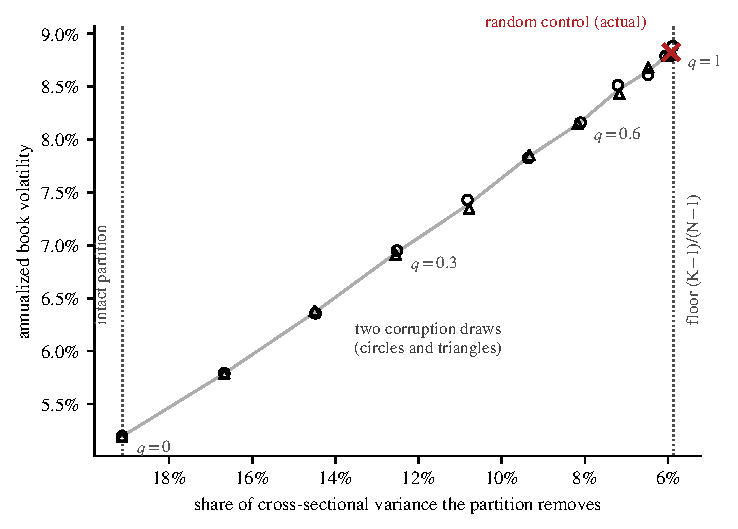
\includegraphics[width=.9\linewidth]{fig_dose}
\caption{Corrupting a real partition, one fraction of labels at a time. This figure plots book volatility against the share of cross-sectional variance the corrupted partition removes. Each point is a full $6{,}913$-day rule-based backtest of the
PCA-loadings partition with a fraction $q$ of each day's labels
redrawn uniformly; two independent corruption draws per $q$ nearly
coincide. The horizontal axis is the share of cross-sectional
variance the corrupted partition removes; the dashed verticals mark
the degrees-of-freedom floor $(\K-1)/(\N-1)$ and the intact partition's
share. The cross is the random control itself.}
\label{fig:dose}
\end{figure}

\subsection{The Estimation Window}
\label{app:window}



Random matrix theory supplies a reason the two clusterizers that gain should be the
sensitive ones: both read individual eigenvectors of the sample
correlation matrix, and at $\N = 500$ a population eigenvalue must exceed $1 + \sqrt{\N/T}$ to be recoverable at all \citep{baik2005phase}. The threshold is $5.9$ at $T = 21$, under which only the market mode survives, against $2.4$ at $T = 252$, under which sector-scale structure does. A rival explanation, however, fits the same six observations, three clusterizers at two windows. The largest gains go to the clusterizers that started lowest, and a regression of the gain on the $21$-day starting level fits with $r = -0.93$. The two explanations make the same prediction on every arm in the sweep. We therefore registered, in advance, three arms on
which they differ by construction, and ran them. Average linkage at
$\K=10$ starts low, so the rival predicts a large gain and the
eigenvector account almost none; the observed gain is $+0.04$. The random
control starts lowest of all, so the rival must predict the largest
gain in the design, while the labels are drawn by a random number
generator that cannot read the window; the observed gain is $-0.11$, negative in four of the five seeds. PCA loadings at $\K=50$ reads eigenvectors, so both accounts predict a gain; the observed gain is $+0.33$. The eigenvector account survives, since it predicts which arms move and in which direction,
and the two arms that use no eigenvector do not move. The account misses the sign of the interaction with $\K$: for PCA loadings the same 60-to-$252$-day move is worth
$+0.27$ at $\K=30$ against $+0.33$ at $\K=50$, so the window effect strengthens as the partition is refined. We have no account of that.

Average linkage peaks at 120 days, mid-sweep; \figref{fig:window_twin} shows the $60$-to-$21$-day step of the same sweep against seed noise. That step shows the account's one exception: complete linkage, which reads the same correlation matrix as average linkage and no eigenvector, loses $0.31$, outside its across-seed band. No $p$-value is quoted for the window responses: a paired test across five fits rests on four degrees of freedom, so each step is judged against its arm's own across-seed band instead.

\begin{figure}[tb]
\centering
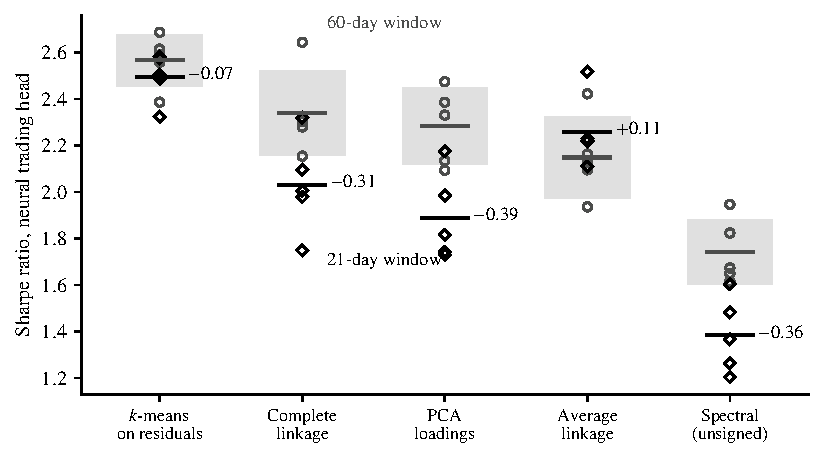
\includegraphics[width=.9\linewidth]{fig_window_twin}
\caption{Changing only the estimation window. This figure plots the per-seed Sharpe ratio at the trained component of the $60$-day arm (circles) against its $21$-day variant (diamonds); the shaded band spans $\pm 1$ across-seed standard deviation of the $60$-day arm, and the horizontal lines are the two windows' seed means. All five $21$-day variants of \appref{app:names} are shown. The two clusterizers that read individual eigenvector coordinates lose $0.39$ and $0.36$, about two and a half times their own band, and complete linkage loses $0.31$; $k$-means on returns moves $-0.07$ and average linkage $+0.11$, both inside their own band.}
\label{fig:window_twin}
\end{figure}

\subsection{Robustness of the Cross-Sectional Projection}
\label{app:lensrobust}

The measurement depends on how many principal components to project
out and which floor to judge the result against. Estimating
the number of factors is a literature of its own \citep{bai2002determining,
onatski2010determining, ahn2013eigenvalue}, and we do not enter it.
At $m = 1, 3, 10$ the $k$-means partition retains $83\%$, $68\%$, $50\%$, and every real partition keeps a strictly positive
excess over its floor at every $m$ tested: the sign of the result is
robust to $m$; the magnitude is not. The floor must also be matched to the partition's own shape. Net of it, retention at five components is $28\%$ to $49\%$ across the 12 clusterizers, and \textsc{gics}, with 10 realized groups on a $322$-name universe, has a floor of $0.028$, not the $0.060$ of \secref{sec:lens}. Against the wrong floor its net retention at 10
components would come out negative, an artifact of over-subtraction. Two details of the protocol qualify these numbers. The retention ratio divides two $R^2$s with different denominators: the share of the post-projection remainder is not a variance decomposition of the original cross-section. The measurement here also counts every group, singletons included, each of which fits its own member exactly. Under the trading convention of \secref{sec:methods}, which deletes singleton members, $k$-means on returns measures $0.264$ on the traded universe with singletons counted (\secref{sec:mechanism}) and $0.216$ without them, against the $0.265$ here.

\subsection{Size of the Spanning Tests}
\label{app:size}

The $t$-statistics of the FF5+MOM block of \tabref{tab:spanning} divide by a Newey--West long-run variance at $21$ lags, and with heavy tails and serial dependence a test of this form can reject more often than its nominal level. We measure its size directly. For each of the 28 books, the null distribution is rebuilt from block-resampled residuals ($21$-day blocks, $5{,}000$ replications per book under each of four independent seeds), with the factor matrix held at its sample values and the betas re-estimated on every draw. The empirical size at nominal $5\%$ is $6.6\%$ pooled across the books and $5.3\%$ to $7.6\%$ book by book. The spread comes from the denominator: dependence cumulated over the $21$ lags is about $1.7$ times as large in the trained books, so the trained books over-reject more. Correcting the size moves the critical value from $1.96$ to $2.2$ in $t$ units even at the worst-behaved book, and the smallest $t$ in that block is $4.1$ ($2.5$ in the block with the reversal factor), so the rejections are not heavy-tail or dependence artifacts.

\subsection{Distance to the Peer Books and Performance}
\label{app:peerdist}

The share of each clusterizer's payoff variance the two peer books explain
runs from $0.52$ to $0.57$, with a positive relation to the clusterizer's Sharpe ratio that falls just short of the $5\%$ level (Spearman $\rho = 0.57$, $p = 0.051$). The overlap between a
clusterizer's positions and the peer books' runs from $0.43$ to $0.48$, or $0.60$ to $0.65$ of what that clusterizer shares with its own refit, with a positive relation to its Sharpe ratio that does not reach significance at the $5\%$ level ($\rho = 0.56$, $p = 0.06$). The two peer books share $0.49$ of their
positions with each other, about as much as either shares with a
clusterizer.

\subsection{Transaction Costs in Detail}
\label{app:costs}

Costs are charged on the positions the runs actually held, so the turnover below is measured from those positions rather than inferred from the payoffs (\appref{app:head}); because the $L^1$ normalization pins the gross book to one (\secref{sec:components}), a position is a share of it. \tabref{tab:costs} reports turnover, the one-way cost at which each book's annual return reaches zero, and net Sharpe ratios at three cost levels. Gross returns run $6.3\%$ to $7.6\%$ a year. At five basis points one-way the same books pay $9.6\%$ to $11.8\%$ a year in cost. Because gross return and cost scale together, the break-even does not depend on leverage.

\begin{table}[tb]
\centering
\caption{Turnover, break-even cost, and net Sharpe ratios}
\label{tab:costs}
\begin{threeparttable}
\small
\setlength{\tabcolsep}{4pt}
\begin{tabular}{@{}lccccccc@{}}
\toprule
& Gross & Return & Turnover & Break-even
& \multicolumn{3}{c}{Net Sharpe ratio} \\
\cmidrule(lr){6-8}
& Sharpe & (\%/yr) & (\%/day) & (bps)
& $1$\,bp & $2$\,bps & $5$\,bps \\
\midrule
12 clusterizers & $1.74$--$2.57$ & $6.62$--$7.60$ & $38.2$--$43.8$ & $3.17$--$3.79$ & $1.20$--$1.86$ & $0.67$--$1.16$ & $-1.24$ to $-0.67$ \\
$\K=1$ & $1.28$ & $6.47$ & $44.6$ & $2.90$ & $0.83$ & $0.38$ & $-0.96$ \\
Random & $1.28$ & $6.25$ & $46.9$ & $2.66$ & $0.79$ & $0.31$ & $-1.15$ \\
\bottomrule
\end{tabular}
\begin{tablenotes}[flushleft]\small
\item \emph{Notes.} This table reports each book's gross Sharpe ratio, annual return, one-way turnover, break-even cost, and net Sharpe ratio at three cost levels. Trained component, five head seeds, each statistic computed per seed and averaged, on the $6{,}913$-day window of \secref{sec:panel} (July 1997 to December 2024). Positions are the weight vectors the runs produced, at gross exposure one. Turnover is one-way, half of
$\sum_i |\Delta w_{it}|$; the break-even and the net columns charge the
full traded notional at the stated one-way rate. Break-even is the one-way rate, in basis points (bps), at which annual return reaches zero. All arms use the common 60-day estimation window of \tabref{tab:methods}; the bands cover the 12 clusterizers, and the two controls are reported on their own rows.
\end{tablenotes}
\end{threeparttable}
\end{table}

The reordering reported in \secref{sec:costs} is not an artifact of the trading head. We run the same measurement on the rule-based component, whose book carries gross exposure two rather than one, and normalize both to the same exposure. Its five-day signal window is rebuilt daily, and its positions correlate with the previous day's at $0.46$ on average across the clusterizers, with $27\%$ of names changing sign. Counted one-way and per unit of gross exposure, the rule-based books turn over $23.1\%$ to $30.8\%$ of their exposure a day against the head's $38.2\%$ to $46.9\%$, and earn $3.9\%$ to $4.6\%$ a year against the head's $6.3\%$ to $7.6\%$. The head trades $1.46$ times as much per unit of exposure and earns $1.63$ times as much, and the two nearly cancel: break-even at the rule-based component is $2.75$ to $3.74$ basis points against $2.66$ to $3.79$ at the trained component. The reordering is sharper without the head: on the rule-based component the two controls finish first and third at five basis points, against ninth and thirteenth at the trained component.

The nearest published comparison runs the other way, and we cannot reconcile the two. \citet{brutti2026orthogonal} report that clustering cuts turnover sharply in their setup, from $87.9\%$ to between $24.2\%$ and $24.4\%$, and charge no costs; our configurations show a far smaller gap, the $\K=1$ control turning over $44.6\%$ against a clustered range of $38.2\%$ to $43.8\%$. Rebalancing frequency is the likely cause (our books are rebuilt every day), but we have not measured it, and we record the divergence as an open question rather than a finding.

Four limitations apply. The cost model is a proportional one-way charge with no market-impact term, and a book rebuilt daily on 500 names is where market impact would be largest. Borrow costs on the short side are not modeled. The panel is US large capitalizations, the most liquid case available, so the break-even here is an upper bound for the same design on a broader universe. Finally, the cost figures are at $\K=30$ only; whether the ordering above survives the sweep of \appref{app:ksweep} is unmeasured.

\end{appendices}

\end{document}
